
\documentclass[a4paper,12pt,twoside]{report}
\usepackage[left=2cm,right=2cm,top=2cm,bottom=3cm]{geometry}
% package that will be used
\usepackage{booktabs}       % professional-quality tables
\usepackage{amsfonts}       % blackboard math symbols
\usepackage{nicefrac}       % compact symbols for 1/2, etc.
\usepackage{microtype}      % microtypography
\usepackage{algorithm}
\usepackage{algorithmic}
\usepackage{amsmath,amssymb}
\usepackage{graphicx}
\usepackage{booktabs}
\usepackage{dsfont}
\usepackage[super]{nth}
\usepackage{etoolbox}
\usepackage{hyperref}
\usepackage{subcaption}

% declare math operator
\DeclareMathOperator{\sgn}{sgn}
\DeclareMathOperator{\clip}{clip}
% new command
\newcommand\Tau{\mathcal{T}}
\newcommand{\norm}[1]{\left\lVert#1\right\rVert}



\usepackage{graphicx}
\usepackage{verbatim}
\usepackage{latexsym}
\usepackage{mathchars}
\usepackage{setspace}

\setlength{\parskip}{\medskipamount}  % a little space before a \par
\setlength{\parindent}{0pt}	      % don't indent first lines of paragraphs

%UHEAD.STY  If this is included after \documentstyle{report}, it adds
% an underlined heading style to the LaTeX report style.
% \pagestyle{uheadings} will put underlined headings at the top
% of each page. The right page headings are the Chapter titles and
% the left page titles are supplied by \def\lefthead{text}.

% Ted Shapin, Dec. 17, 1986

\makeatletter
\def\chapapp2{Chapter}

\def\appendix{\par
 \setcounter{chapter}{0}
 \setcounter{section}{0}
 \def\chapapp2{Appendix}
 \def\@chapapp{Appendix}
 \def\thechapter{\Alph{chapter}}}

\def\ps@uheadings{\let\@mkboth\markboth
% modifications
\def\@oddhead{\protect\underline{\protect\makebox[\textwidth][l]
		{\sl\rightmark\hfill\rm\thepage}}}
\def\@oddfoot{}
\def\@evenfoot{}
\def\@evenhead{\protect\underline{\protect\makebox[\textwidth][l]
		{\rm\thepage\hfill\sl\leftmark}}}
% end of modifications
\def\chaptermark##1{\markboth {\ifnum \c@secnumdepth >\m@ne
 \chapapp2\ \thechapter. \ \fi ##1}{}}%
\def\sectionmark##1{\markright {\ifnum \c@secnumdepth >\z@
   \thesection. \ \fi ##1}}}
\makeatother



%%From: marcel@cs.caltech.edu (Marcel van der Goot)
%%Newsgroups: comp.text.tex
%%Subject: illegal modification of boxit.sty
%%Date: 28 Feb 92 01:10:02 GMT
%%Organization: California Institute of Technology (CS dept)
%%Nntp-Posting-Host: andromeda.cs.caltech.edu
%%
%%
%%Quite some time ago I posted a file boxit.sty; maybe it made it
%%to some archives, although I don't recall submitting it. It defines
%%	\begin{boxit}
%%	...
%%	\end{boxit}
%%to draw a box around `...', where the `...' can contain other
%%environments (e.g., a verbatim environment). Unfortunately, it had
%%a problem: it did not work if you used it in paragraph mode, i.e., it
%%only worked if there was an empty line in front of \begin{boxit}.
%%Luckily, that is easily corrected.
%%
%%HOWEVER, apparently someone noticed the problem, tried to correct it,
%%and then distributed this modified version. That would be fine with me,
%%except that:
%%1. There was no note in the file about this modification, it only has my
%%   name in it.
%%2. The modification is wrong: now it only works if there is *no* empty
%%   line in front of \begin{boxit}. In my opinion this bug is worse than
%%   the original one.
%%
%%In particular, the author of this modification tried to force an empty
%%line by inserting a `\\' in the definition of \Beginboxit. If you have
%%a version of boxit.sty with a `\\', please delete it. If you have my
%%old version of boxit.sty, please also delete it. Below is an improved
%%version.
%%
%%Thanks to Joe Armstrong for drawing my attention to the bug and to the
%%illegal version.
%%
%%                                          Marcel van der Goot
%% .---------------------------------------------------------------
%% | Blauw de viooltjes,                    marcel@cs.caltech.edu
%% |    Rood zijn de rozen;
%% | Een rijm kan gezet
%% |    Met plaksel en dozen.
%% |


% boxit.sty
% version: 27 Feb 1992
%
% Defines a boxit environment, which draws lines around its contents.
% Usage:
%   \begin{boxit}
%	... (text you want to be boxed, can contain other environments)
%   \end{boxit}
%
% The width of the box is the width of the contents.
% The boxit* environment behaves the same, except that the box will be
% at least as wide as a normal paragraph.
%
% The reason for writing it this way (rather than with the \boxit#1 macro
% from the TeXbook), is that now you can box verbatim text, as in
%   \begin{boxit}
%   \begin{verbatim}
%   this better come out in boxed verbatim mode ...
%   \end{verbatim}
%   \end{boxit}
%
%						Marcel van der Goot
%						marcel@cs.caltech.edu
%

\def\Beginboxit
   {\par
    \vbox\bgroup
	   \hrule
	   \hbox\bgroup
		  \vrule \kern1.2pt %
		  \vbox\bgroup\kern1.2pt
   }

\def\Endboxit{%
			      \kern1.2pt
		       \egroup
		  \kern1.2pt\vrule
		\egroup
	   \hrule
	 \egroup
   }	

\newenvironment{boxit}{\Beginboxit}{\Endboxit}
\newenvironment{boxit*}{\Beginboxit\hbox to\hsize{}}{\Endboxit}

\pagestyle{empty}

\setlength{\parskip}{2ex plus 0.5ex minus 0.2ex}
\setlength{\parindent}{0pt}

\makeatletter  %to avoid error messages generated by "\@". Makes Latex treat "@" like a letter

\linespread{1.5}
\def\submitdate#1{\gdef\@submitdate{#1}}

\def\maketitle{
  \begin{titlepage}{
    %\linespread{1.5}
    \Large Imperial College London\\
    %\linebreak
    Department of Bioengineering
    \rm
    \vskip 3in
    \Large \bf \@title \par
  }
  \vskip 0.3in
  \par
  {\Large \@author}
  \vskip 4in
  \par
  Submitted in part fulfilment of the requirements for the degree of 
  \linebreak
  Doctor of Philosophy in Bioengineering of Imperial College London and
  \linebreak
  the Diploma of Imperial College, \@submitdate
  \vfil
  \end{titlepage}
}

\def\titlepage{
  \newpage
  \centering
  \linespread{1}
  \normalsize
  \vbox to \vsize\bgroup\vbox to 9in\bgroup
}
\def\endtitlepage{
  \par
  \kern 0pt
  \egroup
  \vss
  \egroup
  \cleardoublepage
}

\def\abstract{
  \begin{center}{
    \large\bf Abstract}
  \end{center}
  \small
  %\def\baselinestretch{1.5}
  \linespread{1.5}
  \normalsize
}
\def\endabstract{
  \par
}

\newenvironment{acknowledgements}{
  \cleardoublepage
  \begin{center}{
    \large \bf Acknowledgements}
  \end{center}
  \small
  \linespread{1.5}
  \normalsize
}{\cleardoublepage}
\def\endacknowledgements{
  \par
}

\newenvironment{dedication}{
  \cleardoublepage
  \begin{center}{
    \large \bf Dedication}
  \end{center}
  \small
  \linespread{1.5}
  \normalsize
}{\cleardoublepage}
\def\enddedication{
  \par
}

\def\preface{
    \pagenumbering{roman}
    \pagestyle{plain}
    \doublespacing
}

\def\body{
    \cleardoublepage    
    \pagestyle{uheadings}
    \tableofcontents
    \pagestyle{plain}
    \cleardoublepage
    \pagestyle{uheadings}
    \listoftables
    \pagestyle{plain}
    \cleardoublepage
    \pagestyle{uheadings}
    \listoffigures
    \pagestyle{plain}
    \cleardoublepage
    \pagestyle{uheadings}
    \pagenumbering{arabic}
    \doublespacing
}

\makeatother  %to avoid error messages generated by "\@". Makes Latex treat "@" like a letter


\newcommand{\ipc}{{\sf ipc}}

\newcommand{\Prob}{\bbbp}
\newcommand{\Real}{\bbbr}
\newcommand{\real}{\Real}
\newcommand{\Int}{\bbbz}
\newcommand{\Nat}{\bbbn}

\newcommand{\NN}{{\sf I\kern-0.14emN}}   % Natural numbers
\newcommand{\ZZ}{{\sf Z\kern-0.45emZ}}   % Integers
\newcommand{\QQQ}{{\sf C\kern-0.48emQ}}   % Rational numbers
\newcommand{\RR}{{\sf I\kern-0.14emR}}   % Real numbers
\newcommand{\KK}{{\cal K}}
\newcommand{\OO}{{\cal O}}
\newcommand{\AAA}{{\bf A}}
\newcommand{\HH}{{\bf H}}
\newcommand{\II}{{\bf I}}
\newcommand{\LL}{{\bf L}}
\newcommand{\PP}{{\bf P}}
\newcommand{\PPprime}{{\bf P'}}
\newcommand{\QQ}{{\bf Q}}
\newcommand{\UU}{{\bf U}}
\newcommand{\UUprime}{{\bf U'}}
\newcommand{\zzero}{{\bf 0}}
\newcommand{\ppi}{\mbox{\boldmath $\pi$}}
\newcommand{\aalph}{\mbox{\boldmath $\alpha$}}
\newcommand{\bb}{{\bf b}}
\newcommand{\ee}{{\bf e}}
\newcommand{\mmu}{\mbox{\boldmath $\mu$}}
\newcommand{\vv}{{\bf v}}
\newcommand{\xx}{{\bf x}}
\newcommand{\yy}{{\bf y}}
\newcommand{\zz}{{\bf z}}
\newcommand{\oomeg}{\mbox{\boldmath $\omega$}}
\newcommand{\res}{{\bf res}}
\newcommand{\cchi}{{\mbox{\raisebox{.4ex}{$\chi$}}}}
%\newcommand{\cchi}{{\cal X}}
%\newcommand{\cchi}{\mbox{\Large $\chi$}}

% Logical operators and symbols
\newcommand{\imply}{\Rightarrow}
\newcommand{\bimply}{\Leftrightarrow}
\newcommand{\union}{\cup}
\newcommand{\intersect}{\cap}
\newcommand{\boolor}{\vee}
\newcommand{\booland}{\wedge}
\newcommand{\boolimply}{\imply}
\newcommand{\boolbimply}{\bimply}
\newcommand{\boolnot}{\neg}
\newcommand{\boolsat}{\!\models}
\newcommand{\boolnsat}{\!\not\models}


\newcommand{\op}[1]{\mathrm{#1}}
\newcommand{\s}[1]{\ensuremath{\mathcal #1}}

% Properly styled differentiation and integration operators
\newcommand{\diff}[1]{\mathrm{\frac{d}{d\mathit{#1}}}}
\newcommand{\diffII}[1]{\mathrm{\frac{d^2}{d\mathit{#1}^2}}}
\newcommand{\intg}[4]{\int_{#3}^{#4} #1 \, \mathrm{d}#2}
\newcommand{\intgd}[4]{\int\!\!\!\!\int_{#4} #1 \, \mathrm{d}#2 \, \mathrm{d}#3}

% Large () brackets on different lines of an eqnarray environment
\newcommand{\Leftbrace}[1]{\left(\raisebox{0mm}[#1][#1]{}\right.}
\newcommand{\Rightbrace}[1]{\left.\raisebox{0mm}[#1][#1]{}\right)}

% Funky symobols for footnotes
\newcommand{\symbolfootnote}{\renewcommand{\thefootnote}{\fnsymbol{footnote}}}
% now add \symbolfootnote to the beginning of the document...

\newcommand{\normallinespacing}{\renewcommand{\baselinestretch}{1.5} \normalsize}
\newcommand{\mediumlinespacing}{\renewcommand{\baselinestretch}{1.2} \normalsize}
\newcommand{\narrowlinespacing}{\renewcommand{\baselinestretch}{1.0} \normalsize}
\newcommand{\bump}{\noalign{\vspace*{\doublerulesep}}}
\newcommand{\cell}{\multicolumn{1}{}{}}
\newcommand{\spann}{\mbox{span}}
\newcommand{\diagg}{\mbox{diag}}
\newcommand{\modd}{\mbox{mod}}
\newcommand{\minn}{\mbox{min}}
\newcommand{\andd}{\mbox{and}}
\newcommand{\forr}{\mbox{for}}
\newcommand{\EE}{\mbox{E}}

\newcommand{\deff}{\stackrel{\mathrm{def}}{=}}
\newcommand{\syncc}{~\stackrel{\textstyle \rhd\kern-0.57em\lhd}{\scriptstyle L}~}

\def\coop{\mbox{\large $\rhd\!\!\!\lhd$}}
\newcommand{\sync}[1]{\raisebox{-1.0ex}{$\;\stackrel{\coop}{\scriptscriptstyle
#1}\,$}}

\newtheorem{definition}{Definition}[chapter]
\newtheorem{theorem}{Theorem}[chapter]

\newcommand{\Figref}[1]{Figure~\ref{#1}}
\newcommand{\fig}[3]{
 \begin{figure}[!ht]
 \begin{center}
 \scalebox{#3}{\includegraphics{figs/#1.ps}}
 \vspace{-0.1in}
 \caption[ ]{\label{#1} #2}
 \end{center}
 \end{figure}
}

\newcommand{\figtwo}[8]{
 \begin{figure}
 \parbox[b]{#4 \textwidth}{
 \begin{center}
 \scalebox{#3}{\includegraphics{figs/#1.ps}}
 \vspace{-0.1in}
 \caption{\label{#1}#2}
 \end{center}
 }
 \hfill
 \parbox[b]{#8 \textwidth}{
 \begin{center}
 \scalebox{#7}{\includegraphics{figs/#5.ps}}
 \vspace{-0.1in}
 \caption{\label{#5}#6}
 \end{center}
 }
 \end{figure}
}

% begin the document
\begin{document}

\title{\LARGE {\bf Sample Efficient Deep Reinforcement Learning and Related Application}\\
 \vspace*{6mm}
}

\author{Tianhong Dai}
\submitdate{December 2021}

\normallinespacing
\maketitle

\preface

\addcontentsline{toc}{chapter}{Abstract}

\begin{abstract}

Text of the Abstract.

\end{abstract}


\cleardoublepage

\addcontentsline{toc}{chapter}{Acknowledgements}

\begin{acknowledgements}

I would like to express my deep gratitude to:

\begin{itemize}
 \item Anil Anthony Bharath: Anil is my supervisor and brings me into an academic research career. During my Ph.D. study, he provided me with plentiful guidance, help and trust in my research. In addition, he has also provided me with valuable suggestions on my career planning. Without him, I would not have been able to achieve the current results.
 \vspace*{3mm}
 \item Kai Arulkumaran: Kai is my closest colleague/collaborator in the BICI group. He has helped me a lot in my research. In addition, he also gives me many suggestions in daily life. He is also my ``leader" in the field of reinforcement learning.
 \vspace*{3mm}
 \item BICI Group Members: I would like to express my gratitude for their daily support.
 \vspace*{3mm}
 \item My parents: From the day I was born, my parents have provided me with unfailing love and support. Without them, I wouldn't be here today.
 \vspace*{3mm}
 \item My wife: From the day we meet, she continually inspires me to chase my dreams and gives me much love and care. During our two years together in the UK, she has been there to guide me through difficult times, to help me with my worries and to allow me to focus on my work. She makes my life so full of hope and joy that no words can express my gratitude and love to her.
 % 从我们认识的那天起,她就给予我充足的关怀以及爱。我们一起在英国的这两年间,她每天为我准备美味的食物以及提供舒适的生活环境,让我能够专注于我自己的工作。也是她让我的生活充满了希望与快乐,再多的文字也表达不出我对她的感激与爱。
\end{itemize}

\end{acknowledgements}


\cleardoublepage

\begin{dedication}
I hereby declare that the content of this thesis is the product of my own research work. The main parts of this thesis have been published in the following list of my publications. I made the major contribution in design, implementation and experiments for these work under the guidance of Prof. Anil Anthony Bharath and some others which have been acknowledged appropriately in text. The information, codes, and former ideas guided from other sources have been cited in a list of references is in the bibliography.
\end{dedication}
% List the publications used in the thesis
\textbf{Publication List}:
\begin{enumerate}
	\item \underline{Tianhong Dai}, Magda Dubois, Kai Arulkumaran, Jonathan Campbell, Cher Bass, Benjamin Billot, Fatmatulzehra Uslu, Vincenzo de Paola, Claudia Clopath, and Anil Anthony Bharath, ``Deep Reinforcement Learning for Subpixel Neural Tracking", International Conference on Medical Imaging with Deep Learning, 2019 (Spotlight).
	\item \underline{Tianhong Dai}, Hengyan Liu, Anil Anthony Bharath, ``Episodic Self-Imitation Learning with Hindsight", Electronics, Special Issue on Deep Reinforcement Learning: Methods and Applications, 2020.
	\item \underline{Tianhong Dai}, Hengyan Liu, Kai Arulkumaran, Guangyu Ren, and Anil Anthony Bharath, ``Diversity‐based Trajectory and Goal Selection with Hindsight Experience Replay", Pacific Rim International Conference on Artificial Intelligence, 2021.
	\item \underline{Tianhong Dai}, Yali Du, Meng Fang, and Anil Anthony Bharath, ``Diversity-Augmented Intrinsic Motivation for Deep Reinforcement Learning", Neurocomputing, 2021.
	\item \underline{Tianhong Dai}, Kai Arulkumaran, Tamara Gerbert, Samyakh Tukra, Feryal Behbahani, and Anil Anthony Bharath, ``Analysing Deep Reinforcement Learning Agents Trained with Domain Randomisation", Neurocomputing, 2022.
\end{enumerate}

% List extra publications
In addition to the above papers, these following publications that I authored/co-authored during my PhD are out of the main scope of this thesis, and are briefly mentioned in the background or future directions.
\begin{enumerate}
	\item Shafa Balaram, Kai Arulkumaran, \underline{Tianhong Dai}, and Anil Anthony Bharath, ``A Maximum Entropy Deep Reinforcement Learning Neural Tracker", International Workshop on Machine Learning in Medical Imaging, 2019.
	\item Yali Du, Lei Han, Meng Fang, \underline{Tianhong Dai}, Ji Liu, and Dacheng Tao, ``LIIR: Learning Individual Intrinsic Reward in Multi-Agent Reinforcement Learning", Advances in Neural Information Processing Systems, 2019.
	\item \underline{Tianhong Dai}, Wei Li, Xilei Cao, Jianzhuang Liu, Xu Jia, Ales Leonardis, Youliang Yan, and Shanxin Yuan, ``Wavelet-Based Network For High Dynamic Range Imaging", Submitted to IEEE Transactions on Imaging Processing, 2021.
\end{enumerate}

\clearpage

\narrowlinespacing

\vspace*{4mm}

`Quote text here.'\\
\\
\emph{Guy Quoted}

\normallinespacing


\body

\chapter{Introduction}

\section{Motivation and Objectives}

Motivation and Objectives here.



\section{Contributions}

Contributions here.


\section{Statement of Originality}

Statement here.


\section{Publications}

Publications here.

\chapter{Background Theory}

\label{ch:background}
In this chapter, the background covered in this thesis is presented according to the following structure: in Section~\ref{ch3:dnn} and Section~\ref{ch3:bp}, we first briefly discuss deep neural network (DNN), back-propagation and optimisation methods. Then, in Section~\ref{ch3:rl}, some background to reinforcement learning (RL) is introduced. Next, in Section~\ref{ch3:policy-optim}, we discuss more details about policy optimisation in deep reinforcement learning (DRL) and related DRL algorithms that are covered in this thesis. Finally, in Section~\ref{ch3:dpp}, we introduce the fundamentals of determinantal point processes (DPPs).
%Finally, in Section~\ref{ch3:env}, we introduce the benchmark environments which are adopted to evaluate the proposed methods.

\section{Deep Neural Network in DRL}
\begin{figure}[h]
    \centering
    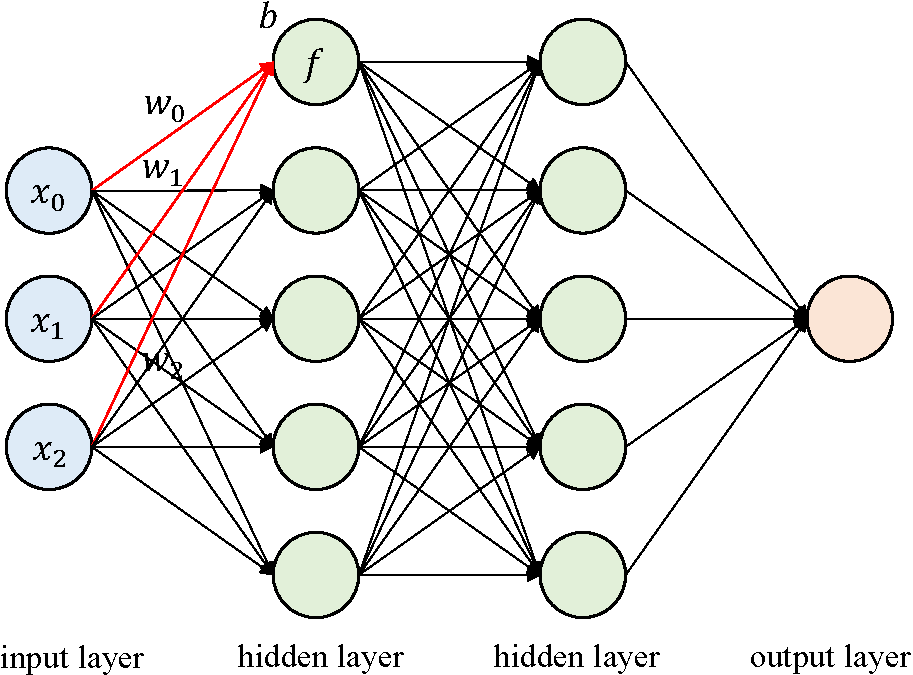
\includegraphics[width=0.7\textwidth]{figures/background/mlp_background.pdf}
    \caption{A simple structure of a multi-layer perceptron (MLP). It consists of an input layer, two hidden layers and an output layer. The highlighted lines (\textcolor{red}{red}) show the connection between a single neuron and its previous layer.}
    \label{fig:nn}
\end{figure}
\label{ch3:dnn}
\subsection{Multi-layer Perceptron}
Deep learning is based on research of artificial neural networks (ANNs). The structure of ANNs is inspired by animal brains, and mimics signal propagation between biological neurons. A feed-forward neural network (FFNN) or multi-layer perceptron (MLP) is a standard structure of ANN, and it consists of several neuron layers, which include an input layer, one or several hidden layers and an output layer (see Figure~\ref{fig:nn}). In each layer, there are multiple neurons, and each neuron is connected to those in the previous layer with corresponding weights $w_{i}$ and a bias $b$. For example, in Figure~\ref{fig:nn}, the transmission of the signal between the highlighted neuron and the previous layer can be expressed as:
\begin{equation}
    f = \sigma (w_{0}x_{0} + w_{1}x_{1} + w_{2}x_{2} + b)
\label{eq:nn_compute}
\end{equation}
here, $\sigma(\cdot)$ represents an activation function, such as a rectifier linear unit (ReLU)~\cite{nair2010rectified}, sigmoid$(\cdot)$ and tanh$(\cdot)$, which are used to add non-linearity to the network, because most real-world problems are nonlinear. The hidden layers in a neural network are used to learn various non-linear combinations of the input data, and the learned non-linear combinations are also called features. These features are the key factors to decide the prediction of the network.

The general forward propagation in an MLP that can be described as the following way. Firstly, the input layer receives the input data of a specific task. The input data can be a flattened image or the property of a house (e.g., the number of rooms, location, and area). Then, in each hidden layer, the output of each neuron is computed according to Equation~\eqref{eq:nn_compute}, and this computation proceeds from the first hidden layer to the last hidden layer. Finally, in the output layer, the output of the network can be the probability of each class in a classification task, the predicted value in a regression task, or the policy/predicted state value in a DRL task.

However, the initial parameters (i.e., weights and bias) of a FFNN may not fit a function for solving a specific task. Thus, the parameters need to be updated through a back-propagation method which is discussed in Section~\ref{ch3:bp}.
% CNN
\subsection{Convolutional Neural Network}
Multi-layer perceptrons (MLPs) are somewhat inefficient in dealing with computer vision tasks because of its fully connected structure. As the input size increases, the number of parameters (weight and bias) also increases. Convolutional neural network (CNN)~\cite{lecun1998gradient} alleviates this problem by using learnable kernels/filters, where each filter traverses the entire image. \td{CNNs are a strong inductive bias that reflects translation invariance of the physical world.} Compared with an MLP, the parameters of these kernels are shared, less, and easy to train. In previous works~\cite{krizhevsky2012imagenet,girshick2014rich,detone2016deep}, CNN has demonstrated its better feature representation ability than other hand-crafted methods, such as histogram of oriented gradient (HOG)~\cite{dalal2005histograms} and scale-invariant feature transform (SIFT)~\cite{lowe2004distinctive}. Nowadays, an increased number of powerful network structures have been proposed, such as the VGG network~\cite{simonyan2014very}, the residual network~\cite{he2016deep}, the dense network~\cite{huang2017densely}, and the capsule network~\cite{sabour2017dynamic}. These network structures improve state-of-the-art performance on various benchmark tasks~\cite{deng2009imagenet,everingham2010pascal}. In DRL, CNNs are regularly used to extract features from high-dimensional inputs (e.g., images) for further processing. In this thesis, as in many DRL studies, we put less effort into the design of the network structure.
%\td{[shifting and scaling in-variance makes CNN important]} 

\section{Back-propagation and Optimisation}
\label{ch3:bp}
Gradient descent~\cite{bottou2010large} is a common technique used to update the parameters of the deep neural network (DNN) to fit a model, and it relies on the gradient of an objective function/loss function with respect to the parameters of the network. The gradient can be calculated efficiently through using the back-propagation algorithm~\cite{kelley1960gradient}. In the forward propagation of an MLP with $N$ layers, the output of each hidden layer can be formulated as:
\begin{equation}
    \mathbf{f}_{i} = \sigma(\mathbf{W}_{i-1}\mathbf{f}_{i-1} + \mathbf{b}_{i-1}), \quad i = 1, 2, \cdots, N,
\end{equation}
where $\mathbf{f}_{i}$ is the output of the current hidden layer, $\mathbf{f}_{i-1}$ is the output of the previous hidden layer, and the input is $\mathbf{f}_{0}$; $\mathbf{W}_{i-1}$ and $\mathbf{b}_{i-1}$ are the weights and bias of the current layer, respectively. Then, in this example, we use the squared error as the loss function to calculate the gradient and update the parameters of the network:
\begin{equation}
    \min_{\bm{\theta}}\mathcal{L} = \norm{\mathbf{y} - \mathbf{f}_{N}(\mathbf{x};\bm{\theta})}^{2},
\end{equation}
where $\bm{\theta}$ is the collection of parameters of the network: $\{\mathbf{W_{0}}, \mathbf{b_{0}}, \mathbf{W_{1}}, \mathbf{b_{1}}, \cdots, \mathbf{W_{N-1}}, \mathbf{b_{N-1}}\}$, $\mathbf{y}$ is the ground truth value and $\mathbf{x}$ is the input data. To minimise the error between the ground truth and the prediction, we need to compute the partial derivatives of $\mathcal{L}$ with respect to the parameters $\bm{\theta}_{i}$ of each layer using the chain rule:
\begin{equation}
   \nabla_{\bm{\theta}_{i}}\mathcal{L} = \frac{\partial \mathcal{L}}{\partial \bm{\theta_{i}}} = \frac{\partial \mathcal{L}}{\partial \mathbf{f}_{N}} \frac{\partial\mathbf{f}_{N}}{\partial \mathbf{f}_{N-1}}\cdots \frac{\partial\mathbf{f}_{i+2}}{\partial \mathbf{f}_{i+1}} \frac{\partial\mathbf{f}_{i+1}}{\partial \bm{\theta}_{i}}.
\end{equation}

Once get the gradient $\nabla_{\bm{\theta}}\mathcal{L}$, the parameters $\bm{\theta}$ can be updated in the opposite direction of the gradient with a step size $\eta$ (i.e. learning rate) via gradient descent:
\begin{equation}
    \bm{\theta} \leftarrow \bm{\theta} - \eta\nabla_{\bm{\theta}}\mathcal{L}.
\end{equation}
However, gradient descent requires the calculation of the gradient over all samples, and it is inefficient when the number of samples is large. Stochastic gradient descent (SGD) reduces computational complexity by randomly splitting the entire samples into several minibatches, and each minibatch is comprised of one or more samples. Then, the gradient is computed over each minibatch samples to update the parameters. 
%Furthermore, SGD with momentum~\cite{qian1999momentum} can accelerate the convergence speed on top of standard SGD.
In this thesis, two variants of the SGD method are used to update the parameters of the network: root mean square propagation (RMSProp)~\cite{tieleman2012lecture} and Adam~\cite{kingma2014adam}.

Root mean square propagation (RMSProp) can adaptively adjust the learning rate for different parameters (i.e., per-parameter learning rate) to accelerate the convergence, the update rule can be written as:
\begin{align}
    \mathbf{v} &\leftarrow \beta \mathbf{v} + (1 - \beta)\nabla_{\bm{\theta}}\mathcal{L}\odot\nabla_{\bm{\theta}}\mathcal{L} \label{eq:squared_grad}\\
     \bm{\theta} &\leftarrow \bm{\theta} - \frac{\eta}{\epsilon+\sqrt{\mathbf{v}}}\odot\nabla_{\bm{\theta}}\mathcal{L} \label{eq:rmsprop_update}.
\end{align}
In Equation~\eqref{eq:squared_grad}, $\mathbf{v}$ is the moving average of the squared gradient, $\odot$ is the element-wise multiplication, and $\beta$ is the decay coefficient which indicates the ratio of history information used to compute the average value. In Equation~\eqref{eq:rmsprop_update}, $\epsilon$ is a small value to prevent division by zero, $\frac{1}{(\epsilon + \sqrt{\mathbf{v}})}$ is the weight to balance the learning rate for individual parameter, in doing so, the learning rate for large gradient will decrease to avoid exploding, and the learning rate for small gradient will increase to avoid vanishing.

Adam is a combination of momentum~\cite{qian1999momentum} and RMSProp, and it is the most popular optimiser in DRL community. The update rule of Adam is:
\begin{align}
    \mathbf{m} &\leftarrow \beta_{1} \mathbf{m} + (1 - \beta_{1})\nabla_{\bm{\theta}}\mathcal{L} \label{eq:momentum_adam}\\
    \mathbf{v} &\leftarrow \beta_{2} \mathbf{v} + (1 - \beta_{2})\nabla_{\bm{\theta}}\mathcal{L}\odot\nabla_{\bm{\theta}}\mathcal{L} \label{eq:squared_grad_adam}\\
     \bm{\theta} &\leftarrow \bm{\theta} - \frac{\eta}{\epsilon+\sqrt{\mathbf{v}}}\mathbf{m} \label{eq:adam_update}.
\end{align}
Equation~\eqref{eq:momentum_adam} is the momentum term, $\mathbf{m}$ is the running average of the gradient, and $\beta_{1}$ is the decay coefficient. The momentum term can correct the gradient in the right direction and thus accelerate the convergence. The other parts are similar to RMSProp.

\section{Reinforcement Learning}
\label{ch3:rl}
\subsection{Markov Decision Process}
\begin{figure}[h]
    \centering
    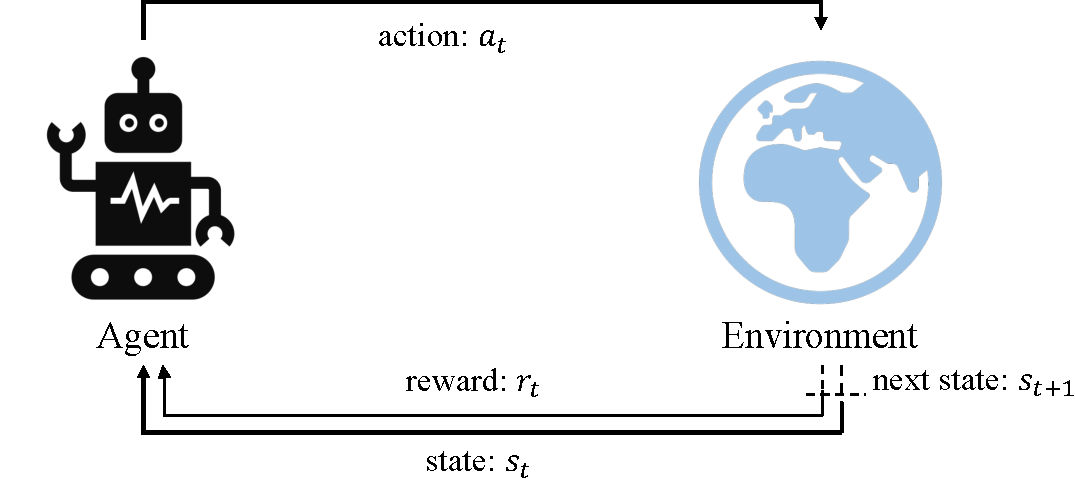
\includegraphics[width=0.8\textwidth]{figures/background/mdp_background.pdf}
    \caption{An overview of reinforcement learning (RL).}
    \label{fig:rl_desc}
\end{figure}
Reinforcement learning (RL) can be formulated under the framework of a Markov Decision Process (MDP); it is used to learn an optimal policy to solve sequential decision-making problems. The MDP is a mathematical framework which describes a fully observable environment in RL, and it is composed of a 5-tuple $<\mathcal{S}, \mathcal{A}, \mathcal{P}, \mathcal{R}, \gamma>$. $\mathcal{S}$ is a set of states, $\mathcal{A}$ is a set of actions, $\mathcal{P}$ is a transition probability/dynamics function: $p(s_{t+1}|s_{t},a_{t})$ which only depends on the current state and action, $\mathcal{R}$ is a reward function, and $\gamma$ is a discount factor. At each timestep $t$, a state $s_{t}\in\mathcal{S}$ is received by an agent from the environment (see Figure~\ref{fig:rl_desc}). An action $a_{t}\in\mathcal{A}$ is sampled by the agent according to its policy $\pi(a_{t}|s_{t})$. Then, the next state $s_{t+1}$ and reward $r_{t}$ are provided to the agent according to the transition function and the reward function. The goal of the RL is to have the agent learn a policy that maximises the expected return $\mathbb{E}_{\pi}[G_{t}]$~\cite{sutton2018reinforcement}:
\begin{equation}
\centering
    G_{t} =\sum_{k=0}^{T-1}\gamma^{k}r_{t+k}.
\label{eq:acc_reward_func}
\end{equation}
Here, the discount factor $\gamma$ exponentially downplays the influence of future rewards. {In a robot manipulation task, the state $s_{t}$ can be the velocity and position of each joint of a robot arm. The action $a_{t}$ can be the velocities of actuators (control signals)} and the reward $r_{t}$ might be calculated based on the distance between the gripper of the robot arm and the target position.

\subsection{Goal-Oriented Reinforcement Learning}
\label{ch3:goal_rl}
The purpose of goal-oriented RL or multi-goal RL is to acquire a policy that can achieve different goals within the environment. 
%Universal Value Function Approximators (UVFA) is proposed to solve such 
In this thesis, the experiments in Chapter~\ref{ch:esil} and Chapter~\ref{ch:dtgsh} follow the terminology suggested by OpenAI~\cite{plappert2018multi}, in which the possible goals are drawn from a goal space $\mathcal{G}$, and the goal being pursued does not influence the environment dynamics. Two types of goal are recognised. One is the desired goal $g\in \mathcal{G}$, which is the target position {or state}, and may be different for different episodes. Within a single episode, $g$ is constant.  The second type of goal is the achieved goal $g^{ac}_{t}$, which is the achieved state in the environment (e.g., the position of an object), and this is considered to be different at each timestep in an episode. In an episode, each transition can be represented as $(s_t|\langle g, g^{ac}_{t} \rangle, a_t, r_t, s_{t+1}|\langle g, g^{ac}_{t+1} \rangle)$, where $s_t$ indicates a state, $a_t$ indicates an action and $r_t$ indicates a~reward; $\langle \, , \rangle$ is simply used to represent the grouping of goals.

\begin{figure}[h]
    \centering
    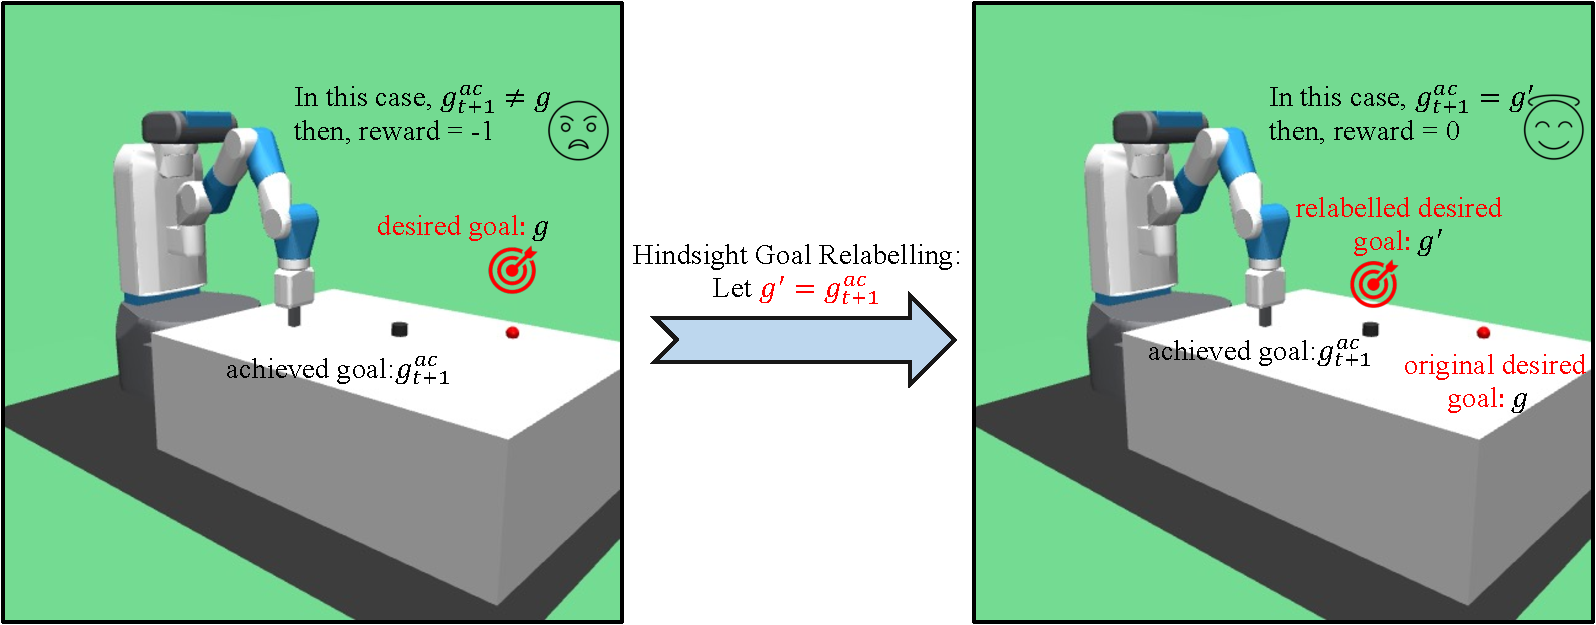
\includegraphics[width=0.85\textwidth]{figures/background/her_background.pdf}
    \caption{A brief illustration of the hindsight goal relabelling in a robotic manipulation task~\cite{plappert2018multi}. In this task, the agent needs to control the gripper to hit the puck and make it slide to a specific position, where the achieved goal is the position of the puck and the desired goal is the target position (the red spot).}
    \label{fig:her_back}
\end{figure}
In sparse reward settings, an agent will only get non-negative rewards when the desired goal $g$ is achieved. The sparse reward function can be defined as:
\begin{equation}
r_{t}\left(g^{ac}_{t+1}, g\right):=
\begin{cases}
0& \text{if $\left\|g^{ac}_{t+1} - g\right\|\leq\epsilon$}\\
-1& \text{otherwise},
\end{cases}
\label{eq:sparse_reward}
\end{equation}
where $\epsilon$ is a threshold value, used to identify if the agent has achieved the goal. {However, the desired goal, $g$, might be difficult to reach during training. Thus, hindsight experiences~\cite{andrychowicz2017hindsight} (see Figure~\ref{fig:her_back}) are created through replacing the original desired goal $g$ with the current achieved goal $g_{t+1}^{ac}$ to augment successful samples, and then reward $r_{t}$ can be recomputed according to Equation~\eqref{eq:sparse_reward}. The modification of the desired goal can be denoted as $g^\prime$ and transitions from hindsight experiences can be represented as $(s_t|\langle g^\prime, g^{ac}_{t} \rangle, a_t, r_t, s_{t+1}|\langle g^\prime, g^{ac}_{t+1} \rangle)$.} {Intuitively, introducing $g^\prime$ serves a useful purpose in the early stages of training; taking, for example, a robot reaching task, the agent has no prior ``concept" of how to move its effector to a specific location in space. Thus, even these original failed episodes contain valuable information for ultimately learning a useful control policy for the original, desired goal $g$.}

\section{Policy Optimisation in DRL}
\label{ch3:policy-optim}
Policy optimisation in DRL can be roughly classified into three categories: 1) value-based methods (see Section~\ref{ch3:value-based}), 2) policy-based methods (see Section~\ref{ch3:policy-based}), and 3) the actor-critic methods, which are the combination of value-based and policy-based methods (see Section~\ref{ch3:actor-critic}).

\subsection{Value-based Methods}
\label{ch3:value-based}
% value based
Value-based methods aim to learn a state or state--action value function instead of an explicit policy. The value function can evaluate the quality of a given state or the quality of an action performed at a given state. Then, the agent can select an action according to the corresponding estimate. This section will discuss how to derive a policy through the value function.

%and for a given state, the agent selects an action according to the prediction of the value function. When the values of states are predicted (i.e. state value function), the agent can select the action towards the next state with the highest state value. When the values of each action are estimated (i.e. state-value function), the agent selects the action with the highest value.

The state value function $V_{\pi}(s_{t})$ under a policy $\pi$ is the expected return when starting from the state $s_{t}$, and can be defined as:
\begin{equation}
\centering
    V_{\pi}(s_{t}) = \mathbb{E}_{\pi}[G_{t}] = \mathbb{E}_{\pi}\biggr[\sum_{k=0}^{T-1} \gamma^{k}r_{t+k}\biggr].
\end{equation}
Through the Bellman equation, the state value function can be rewritten as the combination of the immediate reward, $r_{t}$, and the discounted state value of the next state, $V_{\pi}(s_{t+1})$:
\begin{equation}
\centering
     V_{\pi}(s_{t}) = \mathbb{E}_{\pi}[r_{t} + \gamma V_{\pi}(s_{t+1})].
\end{equation}
% state-action value function
\td{Apart from estimating the state value,} we can also predict the value of a particular state--action pair, denoted as $Q_{\pi}(s_{t},a_{t})$, and this has a similar definition to the state value function:
\begin{equation}
\centering
     Q_{\pi}(s_{t},a_{t}) = \mathbb{E}_{\pi}[G_{t}] = \mathbb{E}_{\pi}\biggr[\sum_{k=0}^{T-1} \gamma^{k}r_{t+k}\biggr].
\end{equation}
The state--action value function $Q_{\pi}(s_{t},a_{t})$ is also called the Q-value function. Similarly, the Q-value function can also be expressed in a recursive form:
\begin{equation}
\centering
     Q_{\pi}(s_{t},a_{t}) = \mathbb{E}_{\pi}[r_{t} + \gamma Q_{\pi}(s_{t+1}, a_{t+1})].
\end{equation}
Next, the optimal policy can be derived using these value functions. In RL, the agent aims to follow the policy that can achieve more accumulated rewards from the environment. Thus, an optimal policy $\pi_{*}$ is defined as the policy that achieves the maximum/optimal state value function, $V_{*}(s_{t})$:
\begin{equation}
    V_{*}(s_{t}) = \max_{\pi}V_{\pi}(s_{t}).
\end{equation}
Similarly, an optimal policy is also defined as the policy that achieves the maximum/optimal Q-value function $Q_{*}(s_{t},a_{t})$:
\begin{equation}
    Q_{*}(s_{t},a_{t}) = \max_{\pi}Q_{\pi}(s_{t},a_{t}).
\end{equation}
Particularly, the optimal policy $\pi_{*}$ can be achieved through this optimal Q-value function directly:
\begin{equation}
    \pi_{*}(s_{t}) = \argmax_{a_{t}} Q_{\pi}(s_{t}, a_{t}).
\end{equation}
Therefore, finding the optimal Q-value function is equivalent to finding the optimal policy. The optimal Q-value function can be reorganised using the Bellman optimality equation:
% bellman optimality equation
\begin{equation}
\centering
     Q_{*}(s_{t},a_{t}) = \mathbb{E}[r_{t} + \gamma\max_{a_{t+1}} Q_{*}(s_{t+1}, a_{t+1})].
\end{equation}
Q-learning~\cite{watkins1992q} is a tabular and iterative update method to solve this equation. In Q-learning, the state--action pairs and corresponding Q-values are stored in a table. For a given state, the action is selected with an exploration strategy (e.g., $\epsilon$-greedy) to observe the next state and the reward, and the Q-value of the current state is updated via:
\begin{equation}
    Q_{\pi}(s_{t}, a_{t}) \leftarrow Q_{\pi}(s_{t}, a_{t}) + \alpha(r_{t} + \gamma\max_{a_{t+1}}Q_{*}(s_{t+1}, a_{t+1}) - Q_{\pi}(s_{t}, a_{t})),
\end{equation}
where $\alpha$ is the learning rate, and this process is repeated until the estimated Q-value converges to the optimal Q-value.

\subsubsection{Function Approximator and Deep Q-Network}
\td{Q-learning in its tabular form}, is impractical to scale to tasks with high-dimensional states, such as playing a video game using images as inputs. The Deep Q-Network (DQN)~\cite{mnih2015human} overcomes this difficulty by combining deep learning and Q-learning. In DQN, instead of updating the Q-value function in a table, a convolutional neural network (CNN) is leveraged to approximate the Q-value function from a stack of images directly:
\begin{equation}
    Q(s_{t},a_{t};\theta) \approx Q^{*}(s_{t},a_{t}),
\end{equation}
here, $\theta$ represents the parameters of a main network. During training, the agent collect samples from the environment with the $\epsilon$-greedy exploration strategy, and each transition ($s_{t}$, $a_{t}$, $r_{t}$, $s_{t+1}$) is stored in a replay buffer $\mathcal{D}$. The replay buffer is designed to reuse past experiences. When updating the parameters $\theta$, a minibatch of transitions is sampled from the replay buffer to minimise the mean squared error (MSE) between the target Q-value and the estimated Q-value using gradient descent methods (e.g., SGD):
\begin{equation}
    \min_{\theta}\mathcal{L} = \mathbb{E}_{(s_{t}, a_{t}, r_{t}, s_{t+1})\sim\mathcal{D}}[(Q(s_{t}, a_{t};\theta) - (r_{t} + \gamma\max_{a_{t+1}}Q(s_{t+1}, a_{t+1};\theta^{-})))^{2}],
\end{equation}
here, $\theta^{-}$ is the parameters of a target network, which is used to estimate the target Q-value. The target network has the same structure as the main network, and its parameters are copied from the main network at each fixed step. The target network is also used to stabilise the training. 

\subsection{Policy-based Methods}
\label{ch3:policy-based}
% policy based
Policy-based methods learn a policy function $\pi(a_{t}|s_{t};{\theta})$, parameterised by $\theta$, and it directly maps a given state $s_{t}$ to an action $a_{t}$. In discrete control tasks, the output of the policy function is a categorical distribution over the action space. In continuous control tasks, the output of the policy function is often the parameters of a Gaussian distribution. During training, the actions are sampled from the corresponding distribution for exploration. In policy-based methods, the optimal parameters $\theta$ can be found by maximising expected returns in the environment:
\begin{align}
    \max_{\theta}J & = \mathbb{E}_{\pi_{\theta}}[G_{t}] \\
                   & = \sum_{s_{t}\in\mathcal{S}}d(s_{t})\sum_{a_{t}\in\mathcal{A}}\pi(a_{t}|s_{t};\theta)G_{t},
\end{align}
where $d(s_{t})$ is the stationary distribution in the Markov chain under the policy $\pi_{\theta}$. In order to maximise the expected returns, we need to increase the probability of the actions which lead to higher returns, and the gradient of the objective function can be expressed as:
\begin{align}
    \nabla_{\theta} J &= \sum_{s_{t}\in\mathcal{S}}d(s_{t})\sum_{a_{t}\in\mathcal{A}}\nabla_{\theta}\pi(a_{t}|s_{t};\theta)G_{t} \\
    &= \sum_{s_{t}\in\mathcal{S}}d(s_{t})\sum_{a_{t}\in\mathcal{A}}\pi(a_{t}|s_{t};\theta)\frac{\nabla_{\theta}\pi(a_{t}|s_{t};\theta)}{\pi(a_{t}|s_{t};\theta)}G_{t}\\
    &= \sum_{s_{t}\in\mathcal{S}}d(s_{t})\sum_{a_{t}\in\mathcal{A}}\pi(a_{t}|s_{t};\theta)\nabla_{\theta}\log\pi(a_{t}|s_{t};\theta)G_{t} \\
    &=\mathbb{E}_{\pi_{\theta}}[\nabla_{\theta}\log\pi(a_{t}|s_{t};\theta)G_{t}], \label{eq:reinforce}
\end{align}
where Equation~\eqref{eq:reinforce} is also known as REINFORCE~\cite{williams1992simple}, and the parameters are updated via gradient ascent. In practice, the return value $G_{t}$ is calculated using Monte Carlo methods, leads to a high variance in the estimated gradient, and slows the convergence of the policy function. In order to alleviate the above shortcomings, actor-critic methods are introduced. 

\subsection{Actor-Critic Methods}
\label{ch3:actor-critic}
Actor-critic methods combine both policy-based methods and value-based methods. The actor is the policy function $\pi(a_{t}|s_{t};\theta)$ to generate an action for a given state. The critic is the value function $V(s_{t};\psi)$ or Q-value function $Q(s_{t},a_{t};\psi)$ to evaluate the quality of a state or a state--action pair and thus guides the training of the actor. To reduce the variance in policy-based methods, a common practice is to subtract a baseline from the estimated return $G_{t}$~\cite{sutton2018reinforcement}. In REINFORCE, the state value predicted by the critic $V(s_{t};\psi)$ is selected as the baseline:
\begin{equation}
    A(s_{t}, a_{t}) = G_{t} - V(s_{t};\psi),
\end{equation}
where $A(s_{t}, a_{t})$ is an advantage function, and the gradient of the policy function can be rewritten as:
\begin{equation}
    \nabla_{\theta} J = \mathbb{E}_{\pi_{\theta}}[\nabla_{\theta}\log\pi(s_{t},a_{t};\theta)A_{t}].
\end{equation}
The critic can also be updated through minimising the MSE error between the return value $R_{t}$ and the estimated state value $V(s_{t};\psi)$:
\begin{equation}
    \min_{\psi}\mathcal{L} = \mathbb{E}[(G_{t} - V(s_{t};\psi))^2].
    \label{eq:mse}
\end{equation}
This actor-critic method is called advantage actor-critic (A2C). For more efficient training, A2C also utilises multiple CPU workers to collect samples from separate environments to update the actor and the critic~\cite{mnih2016asynchronous}. However, A2C does not perform well in continuous control tasks. In this paper, two actor-critic DRL methods -- deep deterministic policy gradient (DDPG)~\cite{lillicrap2015continuous} and proximal policy gradient (PPO)~\cite{schulman2017proximal} -- are adopted as the base algorithms to address the continuous control tasks.

\subsubsection{Deep Deterministic Policy Gradient}
Unlike the previous policy gradient methods (e.g., A2C) which output a probability distribution over the action space, DDPG outputs an action from the actor directly:
\begin{equation}
    a_{t} = \pi(s_{t}; \theta),
\end{equation}
and the critic is a Q-value function $Q(s_{t}, a_{t};\psi)$ to guide the learning of the actor. During training, noise is added to the action $a_{t}$ to help exploration, and the collected transitions are stored in a replay buffer $\mathcal{D}$. For each update iteration, a minibatch sized transitions is sampled to update the actor and the critic. The actor aims to maximise the expected returns $\mathbb{E}[Q(s_{t}, a_{t};\psi)|_{a_{t}=\pi(s_{t};\theta)}]$ and the gradient of the objective function can be estimated using chain rule:

\begin{align}
    \nabla_{\theta}J &\approx\mathbb{E}_{s_{t}\sim\mathcal{D}}[\nabla_{\theta}Q(s_{t}, a_{t};\psi)|_{a_{t}=\pi(s_{t};\theta)}]\\
    & = \mathbb{E}_{s_{t}\sim\mathcal{D}}[\nabla_{a_{t}}Q(s_{t}, a_{t};\psi)|_{a_{t}=\pi(s_{t};\theta)} \nabla_{\theta}\pi(s_{t};\theta)].
\end{align}
The update of the critic is similar to DQN which minimises the MSE between the target Q-vaule and the estimated Q-value:
\begin{equation}
    \min_{\psi}\mathcal{L} = \mathbb{E}_{(s_{t}, a_{t}, r_{t}, s_{t+1})\sim\mathcal{D}}[(Q(s_{t}, a_{t};\psi) - (r_{t} + \gamma Q(s_{t+1}, \pi(s_{t+1};\theta^{-});\psi^{-})))^{2}],
\end{equation}
where $\theta^{-}$ and $\psi^{-}$ are the parameters of the target actor network and the target critic network, respectively. These two target networks are updated toward the parameters of the two main networks slowly using a moving average scheme:
\begin{align}
    \theta^{-} &= \tau\theta^{-} + (1-\tau)\theta\\
    \psi^{-} &= \tau\psi^{-} + (1-\tau)\psi
\end{align}
here, $\tau\in$(0,1) is a coefficient that decides the updating speed of the target networks. 

\subsubsection{Proximal Policy Optimisation}
Before introducing proximal policy optimisation (PPO), we first review its forerunner -- trust region policy optimisation (TRPO)~\cite{schulman2015trust}. When updating the policy network using gradient-based methods, an inappropriate step size (i.e. learning rate) may lead to a worse policy, and the samples collected by this updated policy may interfere with the further policy improvements. In TRPO, when maximising the expected return of a policy network, an extra Kullback-Leibler (KL) divergence term is used to guarantee a promising step size and to restrict the policy update in a specific (trust) region. This constrained objective function can be expressed as:
\begin{align}
   & \max_{\theta} J = \mathbb{E}_{\pi_{\theta_{old}}}\biggr[\frac{\pi(a_{t}|s_{t};\theta)}{\pi(a_{t}|s_{t};\theta_{old})}A(s_{t},a_{t})\biggr] \\
   & \text{subject to} \enspace \mathbb{E}_{\pi_{\theta_{old}}}[\text{KL}[\pi(\cdot|s_{t};\theta_{old}), \pi(\cdot|s_{t};\theta)]] \leq \delta,
\end{align}
where $\theta$ and $\theta_{old}$ are the parameters of the current policy network and the old policy network, respectively, and $\delta$ is a value to limit changes between policies. This objective function can be solved via the method of Lagrange multipliers. In addition, a line search method can be used to estimate an appropriate step size, with the conjugate gradient method being used to estimate the gradient. Although TRPO achieves great performance in continuous control tasks, it is not flexible to be implemented and it performs poorly on tasks with high-dimensional inputs, such as playing Atari games.

Proximal policy optimisation (PPO) provides a simplified solution of TRPO with a clipped objective function to constrain changes of policy during an update:
\begin{equation}
\centering
\max_{\theta}J = \mathbb{E}_{\theta}\biggr[\min\bigg (\frac{\pi(a_{t}|s_{t};\theta)}{\pi(a_{t}|s_{t};\theta_{old})},
	\clip \bigg(\frac{\pi(a_{t}|s_{t};\theta)}{\pi(a_{t}|s_{t};\theta_{old})}, 1-\epsilon, 1+\epsilon \bigg)\bigg )A(s_t, a_t)\biggr],
\label{eq:standard_ppo}
\end{equation}
where $\epsilon$ represents the clipping ratio. In practice, PPO makes the implementation more accessible and improves the performance in tasks with high-dimensional inputs.

\section{Determinantal Point Processes}
\label{ch3:dpp}
A determinantal point process (DPP)~\cite{kulesza2012determinantal} is a stochastic process that characterises a probability distribution over sets of points using the determinant of some function. In machine learning, it is often used to quantify the diversity of a subset, with applications such as video~\cite{mahasseni2017unsupervised} and document summarisation~\cite{hong2014improving}.

Formally, for a discrete set of points $\mathcal{Y}=\{\mathbf{x}_{1}, \mathbf{x}_{2}, \cdots, \mathbf{x}_{N}\}$, a point process $\mathcal{P}$ is a probability measure over all $2^{|\mathcal{Y}|}$ subsets. $\mathcal{P}$ is a DPP if a random subset $\mathbf{Y}$ is sampled with probability:
\begin{equation}
    \mathcal{P}_{L}(\mathbf{Y}=Y) = \frac{\text{det}(\mathbf{L}_{Y})}{\sum_{Y'\subseteq \mathcal{Y}} \text{det}(\mathbf{L}_{Y'})} = \frac{\text{det}(\mathbf{L}_{Y})}{\text{det}(\mathbf{L}+\mathbf{I})},
\end{equation}
where $Y\subseteq \mathcal{Y}$, $\mathbf{I}$ is the identity matrix, $\mathbf{L} \in \mathbb{R}^{N\times N}$ is the positive semi-definite DPP kernel matrix, and $\mathbf{L}_{Y}$ is the sub-matrix with rows and columns indexed by the elements of the subset $Y$. 

The kernel matrix $\mathbf{L}$ can be represented as the Gram matrix $\mathbf{L} = \mathbf{X}^{T}\mathbf{X}$, where each column of $\mathbf{X}$ is the feature vector of an item in $\mathcal{Y}$. The determinant, $\text{det}(\mathbf{L}_{Y})$, represents the (squared) volume spanned by vectors $\mathbf{x}_{i}\in Y$. From a geometric perspective, feature vectors that are closer to being orthogonal to each other will have a larger determinant, and vectors in the spanned subspace are more likely to be sampled: $\mathcal{P}_{L}(\mathbf{Y}=Y) \propto \text{det}(\mathbf{L}_{Y})$. Using orthogonality as a measure of diversity, we leverage DPPs to sample diverse trajectories and goals in Chapter~\ref{ch:dtgsh}. In Chapter~\ref{ch:daim}, we use DPPs to model an intrinsic motivation, which aims to encourage the agent to explore novel states in the environment.
\chapter{Episodic Self-Imitation Learning with Hindsight}
\label{ch:esil}
\section{Introduction}
% \td{In this chapter, we propose episodic self-imitation learning (ESIL), which aims to address }
%------------------------------ From Main Paper ----------------------------
Reinforcement learning (RL) has been shown to be very effective in training agents within gaming environments~\cite{mnih2015human,silver2016mastering}, particularly when combined with deep neural networks~\cite{lecun2015deep,silver2016mastering,liu2017survey}. In most tasks settings that are solved by RL algorithms, reward shaping is an essential requirement for guiding the learning of the agent. However, reward shaping often requires significant quantities of domain knowledge that {are} highly task-specific~\cite{ng1999policy} and, even with careful design, can lead to undesired policies. Moreover, for complex robot manipulation tasks, the manual design of reward shaping functions to guide the learning agent becomes intractable~\cite{arulkumaran2017deep,florensa2017reverse} if even minor variations are introduced in the task. For such settings, the application of deep reinforcement learning requires algorithms that can learn from unshaped, and usually sparse, reward signals. The complicated dynamics of robot manipulation exacerbates the difficulty posed by sparse rewards, especially for on-policy RL algorithms. For example, achieving goals that require the successful execution of multiple steps over a long horizon involves high-dimensional control that must also be generalised to work across variations in the environment for each step. These aspects of robot control result in a situation where a naive RL agent so rarely receives a reward at the start of training that it cannot learn at all. A common solution in the \td{DRL} community is collecting a sufficient number of expert demonstrations, then use imitation learning to train the agent. However, in some scenarios, demonstrations are expensive to collect and the performance of a trained agent is restricted by their quantity. One solution is to use the valuable past experiences of the agent to improve training, which is particularly useful in sparse reward environments.

There are two kinds of approaches to alleviate the problems associated with sparse rewards: imitation learning and hindsight experience replay (HER)~\cite{andrychowicz2017hindsight}. First, the standard approach of imitation learning is to use supervised learning algorithms and minimise a surrogate loss with respect to an oracle. The most common form is learning from demonstrations~\cite{hester2018deep,gao2018reinforcement}. Similar techniques are applied to robot manipulation tasks~\cite{rajeswaran2017learning,vevcerik2017leveraging,nair2018overcoming,james2018task}. When the demonstrations are not attainable, self-imitation learning (SIL)~\cite{oh2018self}, which uses past good experiences (episodes in which the goal is achieved), can~be used to enhance the exploration or speed up the training of the agent. {Self-imitation learning} works well in discrete control environments, such as Atari games. While being able to learn policies for continuous control tasks with dense or delayed rewards~\cite{oh2018self}, the present experiments suggest that SIL struggles when the rewards are sparse. Recently, {hindsight experience replay} has been proposed to solve such goal-oriented, sparse reward problems. The main idea of HER is that during replay, the selected transitions are sampled from state--action pairs derived from {achieved goals} that are substituted for the real goals of the task; this increases the frequency of positive rewards. {Hindsight experience replay} is used with off-policy RL algorithms, such as DQN~\cite{mnih2015human} and DDPG~\cite{lillicrap2015continuous}, for experience replay and has several extensions~\cite{schaul2015prioritized,liu2018competitive}. The present experiments show that simply applying HER with SIL does not lead to an agent capable of performing tasks from the Fetch robot environment. In summary, self-imitation learning with on-policy algorithms for tasks that require continuous control, and for which rewards are sparse, remains unsolved.

In this chapter, {episodic self-imitation learning (ESIL) for goal-oriented problems that provide only sparse rewards is proposed and combined with a state-of-the-art on-policy RL algorithm:} proximal policy optimisation (PPO). In contrast to standard SIL, which samples past good transitions from the replay buffer for imitation learning, {the proposed} ESIL adopts the entire set of current episodes {(successful or not)}, and modifies them into ``expert'' trajectories based on HER. An extra trajectory selection module is also introduced to relieve the effects of sample correlation~\cite{lee2019sample} in updating the network. Figure~\ref{fig:esil} shows the difference between naive SIL+HER and ESIL. During training by SIL+HER, a batch of transitions is sampled from the replay buffer; these are modified into ``hindsight experiences'' and used directly in self-imitation learning. In contrast, ESIL utilises the entire currently collected episodes and converts them into hindsight episodes. The trajectory selection module removes undesired transitions in the hindsight episodes. Using tasks from the OpenAI Fetch environment~\cite{plappert2018multi}, this chapter demonstrates that the proposed ESIL approach effectively trains the agent which is required to solve continuous control problems, and shows that it achieves state-of-the-art results on several tasks.

\begin{figure}[t]
\centering
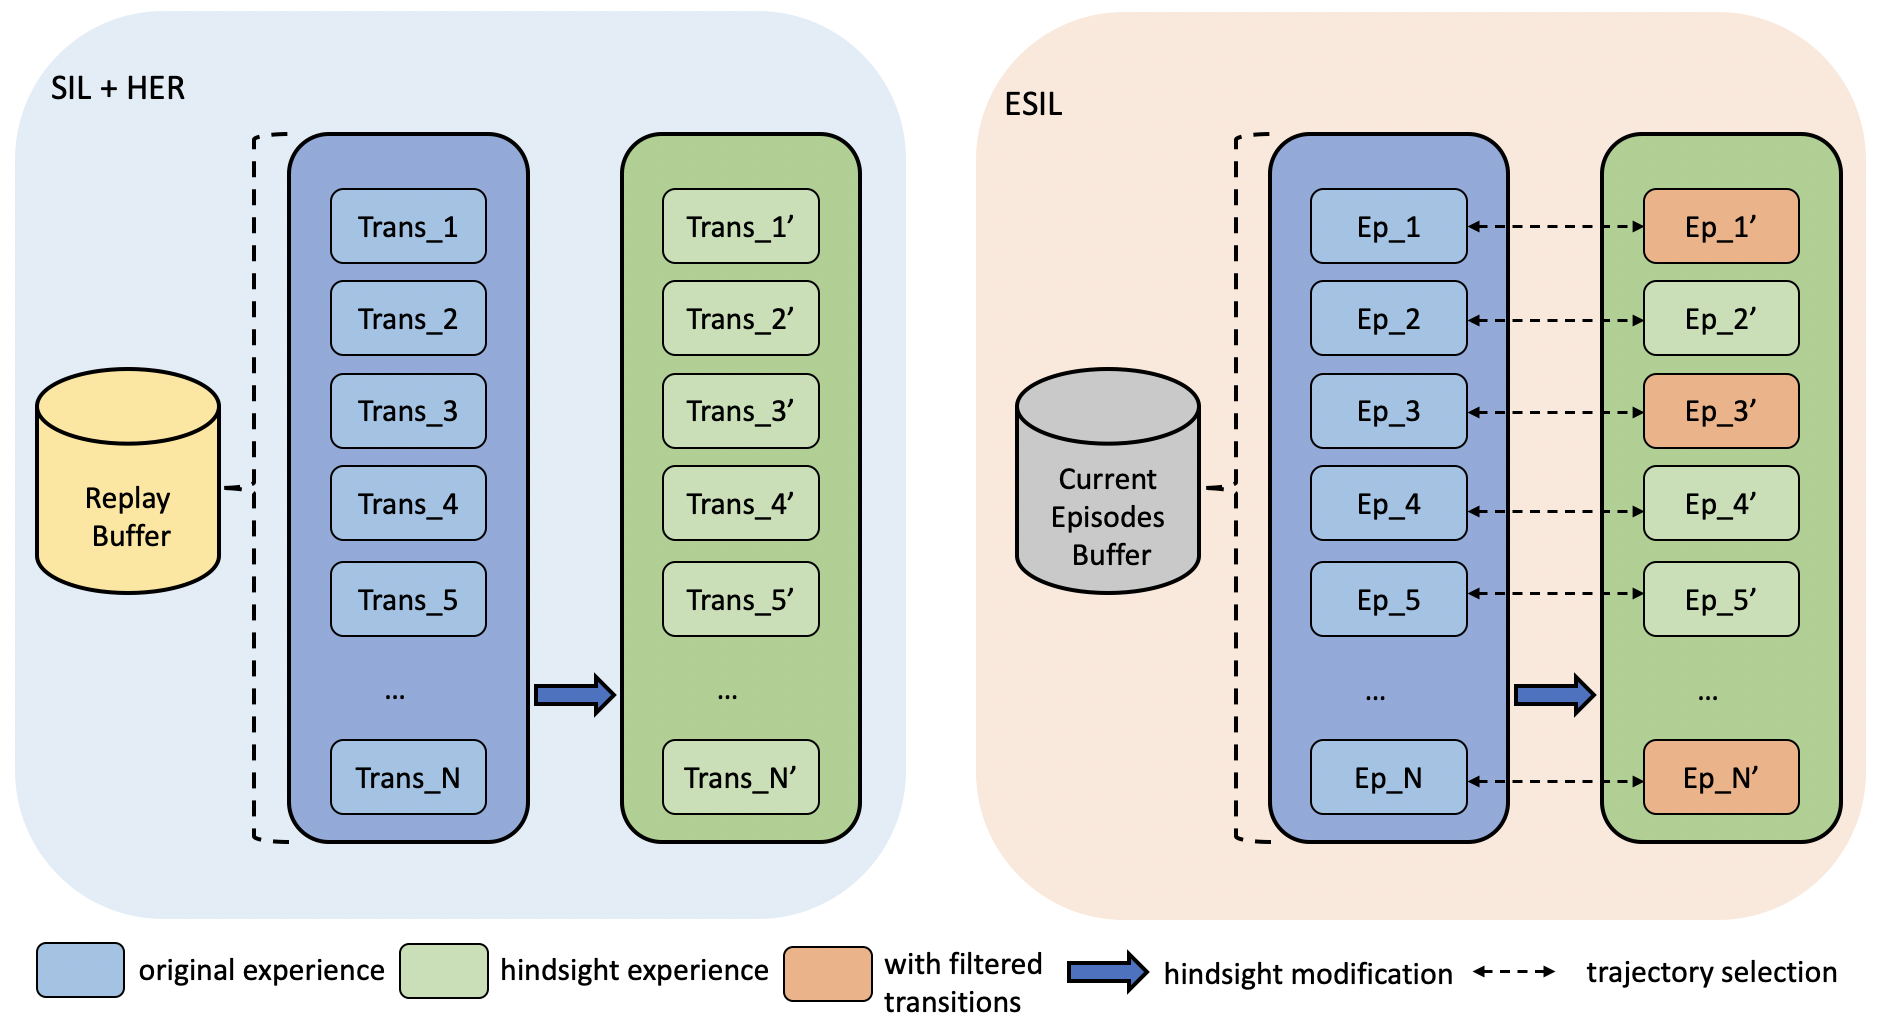
\includegraphics[width=0.95\textwidth]{figures/chapter3/buffer.png}
\caption{Illustration of the difference between self-imitation learning (SIL)+hindsight experience replay (HER) and episodic self-imitation learning (ESIL).}
%% PPO+SIL+HER samples a batch of transitions from the replay buffer and modify them into hindsight experiences and conduct self-imitation learning directly. PPO+ESIL utilizes entire current collected episodes and convert them into hindsight episodes. Another trajectory selection module is used to remove undesired transitions in each hindsight episodes.
\label{fig:esil}
\end{figure}

The primary contribution of this chapter is a novel episodic self-imitation learning (ESIL) algorithm that can solve continuous control problems {in environments providing only sparse rewards}; in doing so, it also empirically answers an open question posed by Plappert \textit{et al.}~\cite{plappert2018multi} -- ``\textit{How to combine HER with state-of-the-art on-policy RL algorithms like
PPO?}". {The proposed ESIL approach also provides} a more efficient way to perform exploration in goal-oriented settings than the standard self-imitation learning algorithm. 
% Finally, to our knowledge, this approach achieves the best results for four moderately complex robot control tasks in simulation. 
Finally, this approach outperforms other on-policy RL algorithms in all simulated robot manipulation tasks.

% Related work
\section{Related Work}
% exploration
Imitation learning (IL) can be divided into two main categories: behavioural cloning and inverse reinforcement learning~\cite{hussein2017imitation}. Behavioural cloning involves the learning of behaviours from demonstrations~\cite{bojarski2016end,xu2017end,torabi2018behavioral}. Other extensions have an expert in the loop, such as DAgger~\cite{ross2011reduction}, or use an adversarial paradigm for the behavioural cloning method~\cite{ho2016generative,wang2017robust}. The inverse reinforcement learning estimates a reward model from expert trajectories~\cite{ng2000algorithms,abbeel2004apprenticeship,ziebart2008maximum}. Learning from demonstrations is powerful for complex robot manipulation tasks~\cite{finn2016guided,zhang2018deep,pmlr-v78-finn17a,rajeswaran2017learning,fang2019survey}. Prior work has used demonstrations to accelerate  learning~\cite{rajeswaran2017learning,vevcerik2017leveraging,nair2018overcoming},  nevertheless demonstrations are often collected by an expert policy or human actions. In contrast to these approaches, {episodic self-imitation learning (ESIL) does not need demonstrations.}

% self-learning and self-imitation learning
Self-imitation learning (SIL)~\cite{oh2018self} can be used for exploiting past experiences for parametric policies. It~has a similar flavor to ~\cite{gangwani2018learning, pmlr-v97-wu19a}, in that the agent learns from imperfect demonstrations. During~training, past good experiences are stored in the replay buffer. When SIL starts, transitions are sampled from the replay buffer according to the advantage values. {In the work of~\cite{tang2020self}, generalised~SIL was proposed as an extension of SIL. It uses an $n$-bound $Q$-learning approach to generalise the original SIL technique, and shows robustness to a wide range of continuous control tasks. Generalised SIL can also be combined with both deterministic and stochastic RL algorithms. Guo \textit{et al.}~\cite{guo2019self} points out that using imitation learning with past successful experiences could lead to a sub-optimal policy. Instead of imitating past good trajectories, a trajectory-conditioned policy~\cite{guo2019self} is proposed to imitate trajectories in diverse directions, encouraging exploration in environments where exploration is otherwise difficult.} Unlike SIL, episodic self imitation learning (ESIL) applies HER to the current episodes to create ``imperfect'' demonstrations for imitation learning; this also requires introducing a trajectory-selection module to reject undesired samples from the hindsight experiences. In the work of~\cite{lee2019sample}, it was shown that the agent benefits from using whole episodes in updates, rather~than uniformly sampling in the sparse or delayed reward environments. The present experiments suggest that episodic self-imitation learning {achieves better performance in an agent that must learn to perform continuous control in environments delivering sparse rewards}.

% Hindsight
Recently, the technique known as hindsight learning has been developed. Hindsight experience replay (HER)~\cite{andrychowicz2017hindsight} is an algorithm that can overcome the exploration problems in multi-goal environments, delivering sparse rewards. Hindsight policy gradient (HPG)~\cite{rauber2018hindsight} introduces techniques that enable the learning of goal-oriented policies using hindsight experiences with on-policy RL algorithms. However, the current implementation of HPG has only been evaluated for agents that need to perform discrete actions, and one drawback of hindsight policy gradient estimators is the computational cost because of the goal-oriented sampling. Unlike HPG, episodic self-imitation learning (ESIL) combines episodic hindsight experiences with imitation learning, which aids learning at the beginning of training. Furthermore, ESIL can be applied to continuous control, making it more suitable for control problems that demand greater precision.

% Methodology
\section{Methodology}
\label{sec:method}
The proposed method combines PPO and episodic self-imitation learning to maximally use hindsight experiences for exploration to improve learning. {Recent advantages in episodic update~\cite{lee2019sample} and hindsight experiences~\cite{andrychowicz2017hindsight} are also leveraged} to guide exploration for on-policy RL. 

\subsection{Episodic Self-Imitation Learning}
The present method aims to use episodic hindsight experiences to guide the exploration of the PPO algorithm. To this end, hindsight experiences are created from current episodes. For an episode $i$, let there be $T$ timesteps; after $T$ timesteps, a series of transitions $\tau_i =\{ (s_{t}, a_{t}, r_{t}, s_{t+1}, g, g^{ac}_{t+1})\}_{t=0:T-1}$ is collected. If at timestep $t=T-1$, in $s_{T}$, $g^{ac}_{T} \neq g$, it implies that in this episode, the agent failed to achieve the original goal. Simply, to create hindsight experiences, {the achieved goal $g^{ac}_{T}$ in the last state $s_{T}$ is selected and considered as the modified desired goal $g^{\prime}$, i.e., $g^\prime = g^{ac}_{T}$.} Next, a new reward $r_{t}^{\prime}$ is computed under the new goal $g^\prime$. Then, {a new ``imagined'' episode is achieved}, and a new series of transitions $\tau_i^{\prime} = \{(s_{t}, a_{t}, r_{t}^{\prime},s_{t+1}, g^\prime, g^{ac}_{t+1})\}_{t=0:T-1}$ is collected.
Then, an approach to self-imitation learning based on episodic hindsight experiences is proposed, which applies the policy updates to both hindsight and in-environment episodes. Proximal policy optimisation (PPO) is used as the base RL algorithm, which is a state-of-the-art on-policy RL algorithm. With current and corresponding hindsight experiences, a new objective function is introduced and defined as:
\begin{equation}
  \centering
  \mathcal{L} = \alpha\mathcal{L}_{PPO} + \beta\mathcal{L}_{ESIL},
  \label{eq:loss}
\end{equation}
where $\alpha$ is the weight coefficient of $\mathcal{L}_{PPO}$. In the experiments, we set $\alpha=1$ as default {to balance the contribution of $\mathcal{L}_{PPO}$ and $\mathcal{L}_{ESIL}$}. $\mathcal{L}_{PPO}$ is the loss of PPO which can be written as:
\begin{equation}
  \mathcal{L}_{PPO} = \mathcal{L}_{policy} - c\mathcal{L}_{value}
  \label{eq:ppo_loss}
\end{equation}
where $\mathcal{L}_{policy}$ is the policy loss which is parameterised by $\theta$, $\mathcal{L}_{value}$ is the value loss which is parameterised by $\psi$, and $c$ is the weight coefficient of the $\mathcal{L}_{value}$, which is set to 1 to match the default PPO setting~\cite{schulman2017proximal}. The policy loss, $\mathcal{L}_{policy}$, can be represented as:
\begin{equation}
  \centering
  \mathcal{L}_{policy} = \mathbb{E}_{s_{t}, a_{t}, g\in\Tau}\biggr[\min \left (\frac{\pi(a_{t}|s_{t}, g;\theta)}{\pi(a_{t}|s_{t}, g;\theta_{old})}A_{t}, \clip \left (\frac{\pi(a_{t}|s_{t}, g;\theta)}{\pi(a_{t}|s_{t}, g;\theta_{old})}, 1-\epsilon, 1+\epsilon \right )A_{t}\right )\biggr],
  \label{eq:policy_loss}
\end{equation}
here, $A_{t}$ is the advantage value, and can be computed as $G_{t} - V(s_{t}, g;\psi)$. $V(s_{t}, g;\psi)$ is the state value at timestep $t$ which is predicted by the critic network. $G_{t}$ is the return at timestep $t$. $\epsilon$ is the clip ratio. $\Tau$~indicates original trajectories. {The value loss is a squared error loss $\mathcal{L}_{value}=\mathbb{E}[(V(s_{t}, g;\psi) - G_{t})^{2}]$.}

For the $\mathcal{L}_{ESIL}$ term, $\beta$ is an adaptive weight coefficient of $\mathcal{L}_{ESIL}$; it can be defined as the ratio of samples which are selected for self-imitation learning:
\begin{equation}
  \beta=\frac{N_{ESIL}}{N_{Total}},
\end{equation}
where $N_{ESIL}$ is the number of samples used for self-imitation learning and $N_{Total}$ is the total number of collected samples.
The episodic self-imitation learning loss $\mathcal{L}_{ESIL}$ can be written as: 
\begin{equation}
  \centering
  \mathcal{L}_{ESIL}=\mathbb{E}_{s_{t}, a_{t}, g^\prime\in\Tau^{'}}\left[\log\pi\left(a_{t}|s_{t}, g^\prime;\theta\right)\mathcal{F}_t\right],
  \label{eq:imitaion}
\end{equation}
where $\Tau^{'}$ denotes hindsight trajectories and $\mathcal{F}_t$ is the trajectory selection module which is based on returns of the current episodes, $G$, and the returns of corresponding hindsight experiences, $G^{\prime}$.

\subsection{Episodic Update with Hindsight}
Two crucial issues of ESIL are: 1) hindsight experiences are sub-optimal, and 2) the {detrimental} effect of updating networks with correlated trajectories. 
Although episodic self-imitation learning makes exploration more effective, hindsight experiences are not from experts and not ``perfect'' demonstrations.  With the training process continuing, if the agent is always learning these imperfect demonstrations, the policy will be stuck at the sub-optimal, or experience overfitting.

To prevent the agent from learning imperfect hindsight experiences, {hindsight experiences are actively selected based on returns.} With the same action, different goals may lead to different results. The proposed method only selects hindsight experiences that can achieve higher returns. The illustration of the trajectory selection module is in Figure~\ref{fig:hs_princple}. For an episodic experience and its hindsight experience, the returns of the episodic experience and its hindsight experience can be calculated, respectively. 
In a trajectory, at each timestep $t$, the return $G_{t}$ can be calculated by $G_{t} = G(s_t, g) = r_{t} + \gamma r_{t+1} + \gamma^{2} r_{t+2} + ... + \gamma^{T-t-1} r_{T-1}$. Then, for a trajectory $\tau_{i}$, we have $\left\{G_{0}^{i}, G_{1}^{i}, G_{2}^{i}, ..., G_{T-1}^{i}\right\}$.

For the hindsight experiences, similarly, the return $G_{t}'$ for each timestep $t$,~with respect to the hindsight goal $g^\prime$, can be calculated. Based on the modified trajectory $\tau_{i}^{\prime}$ with the same length of $\tau_{i}$, we therefore have the returns $\left\{G_{0}^{i^\prime}, G_{1}^{i^\prime}, G_{2}^{i^\prime}, ..., G_{T-1}^{i^\prime}\right\}$. During training, the~hindsight experiences with higher returns are used for self-imitation learning. The rest of the hindsight experiences will be \td{assumed to be of lower importance} and ignored.
Then, Equation~\eqref{eq:imitaion} can be rewritten as:
\begin{equation}
  \centering
  \mathcal{L}_{ESIL}=\mathbb{E}_{s_{t}, a_{t}, g^\prime\in\Tau^{'},g\in\Tau}\biggr[\log\pi_{\theta}\left(a_{t}|s_{t}, g^\prime\right)\mathcal{F}\left(s_{t}, g, g^\prime\right)\biggr],
  \label{eq:final_loss}
\end{equation}
where $\mathcal{F}\left(s_{t}, g, g^{\prime}\right)$ is the trajectory selection module. The selection function can be expressed as
\begin{equation}
  \centering
  \mathcal{F}\left(s_{t}, g, g^\prime \right)=\mathds{1}\left[G(s_{t}, g^\prime) > G(s_{t}, g)\right],
\end{equation}
here, {$\mathds{1}(\cdot)$ is the unit step function}. Consider the OpenAI Fetch environment as an example. For~a failed trajectory, the rewards $r_{t}$ are $\{-1,-1,\cdots, -1\}$. {The desired goal is modified} to construct a new hindsight trajectory, and the new rewards $r_{t}^{\prime}$ become $\{-1,-1,\cdots, 0\}$. Then,  {$G$ and $G^{\prime}$ can be calculated~separately.}
\begin{figure}[t!]
  \centering
  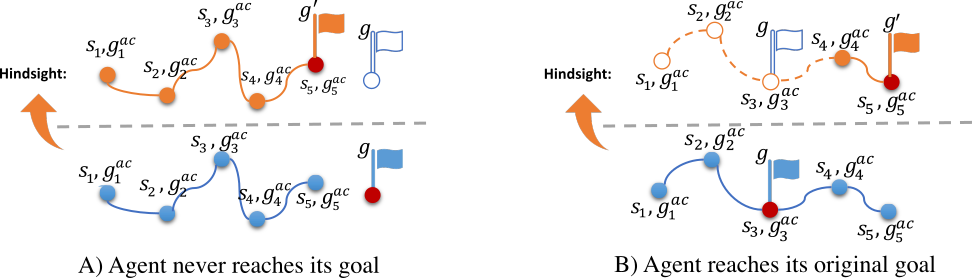
\includegraphics[width=\columnwidth]{figures/chapter3/hgs.png}
  \caption{A simplified illustration of trajectory selection. Blue trajectories indicate original experiences. Orange trajectories indicate hindsight experiences. Solid trajectories in the hindsight experiences are selected by the trajectory selection module of ESIL with new ``imagined'' goals.}
  \label{fig:hs_princple}
\end{figure}

From a goal perspective, episodic self-imitation learning (ESIL) tries to explore (desired) goals to get positive returns.~It can be viewed as a form of multi-task learning, {because ESIL has two objective functions to be optimised jointly.}~It is also related to self-imitation learning (SIL)~\cite{oh2018self}.~However,~ the~difference is that SIL uses $\left(G-V(s;\theta)\right)_{+}$ on past experiences to learn to choose the action chosen in the past in a given state, rather than goals. The full description of ESIL can be found in Algorithm~\ref{alg}.
% the algorithm
\begin{algorithm}[t!]
  \caption{Proximal Policy Optimisation (PPO) with Episodic Self-Imitation Learning (ESIL)}
  \label{alg}
  \begin{algorithmic}[1]
    \REQUIRE an actor network $\pi(s, g;\theta)$, a critic network $V(s, g;\psi)$, the maximum steps $T$ of an episode, a reward function $\mathcal{R}$, number of iterations $N$, number of episodes for each iteration $M$, weight coefficient of critic loss term $c$, weight coefficient of PPO term $\alpha$, adaptive coefficient $\beta$  
    %\STATE Initialize the parameters $\theta$ and $\psi$ of both actor and critic networks
    \FOR{$\mathrm{iteration} = 1, 2, \cdots N$}
    \STATE $\Tau \leftarrow \varnothing$, $\Tau^{\prime} \leftarrow \varnothing$ 
    \FOR{$\mathrm{episode} = 1, 2, ..., M$}
    \STATE $\tau \leftarrow \varnothing$
    \FOR{$t = 0, 1, \cdots, T-1$}
    \STATE Sample an action $a_{t}$ using the actor network $\pi(s_{t}, g;\theta)$
    \STATE Execute the action $a_{t}$ and observe a new state $s_{t+1}$
    \STATE Store the transition $\left(s_{t}, a_{t}, r_{t}, s_{t+1}, g^{ac}_{t+1}\right)$ in $\tau$
    \ENDFOR

    \FOR{\textbf{each} transition $\left(s_{t}, a_{t}, r_{t}, g, g^{ac}_{t+1} \right)$ in $\tau$}
    \STATE Clone the transition and replace $g$ with $g^{\prime}$, where $g^{\prime}=g^{ac}_{T}$
    \STATE $r_{t}^{\prime}:=\mathcal{R}\left(s_{t}, a_{t}, g^{\prime}\right)$
    \STATE Store the transition $\left(s_{t}, a_{t}, r_{t}^{\prime}, g^{\prime}, g^{ac}_{t+1}\right)$ in $\tau^{\prime}$
    \ENDFOR
    % next loop
    \STATE Store the trajectory $\tau$ and the hindsight trajectory $\tau^{\prime}$ in $\Tau$ and $\Tau^{\prime}$, respectively 
    \ENDFOR

    \STATE Calculate the Returns $G$ and $G^{\prime}$ for all transitions in $\Tau$ and $\Tau^{\prime}$, respectively
    \STATE Calculate the PPO loss: $\mathcal{L}_{PPO} = \mathcal{L}_{policy} - c\mathcal{L}_{value}$
    \STATE Calculate the ESIL loss: $\mathcal{L}_{ESIL}$ using Eq.\eqref{eq:imitaion}
    \STATE Update the parameters $\theta$ and $\psi$ using loss $\mathcal{L}=\alpha\mathcal{L}_{PPO} + \beta\mathcal{L}_{ESIL}$
    \ENDFOR 
\end{algorithmic}
\end{algorithm}

\section{Experiments}
\label{sec:experiment}
The proposed method is evaluated on several multi-goal environments, including the Empty Room environment and the OpenAI Fetch environment (see Figure~\ref{fig:env}). The Empty Room environment is a toy example, and has discrete action spaces. In the Fetch environment, there are four robot tasks with continuous action spaces. To obtain a comprehensive comparison between the proposed method and other baselines, suitable baselines are selected for different environments. In addition, ablation studies of the trajectory selection module are also performed.
\begin{figure}[t]
\minipage{0.19\textwidth}
  \centering
  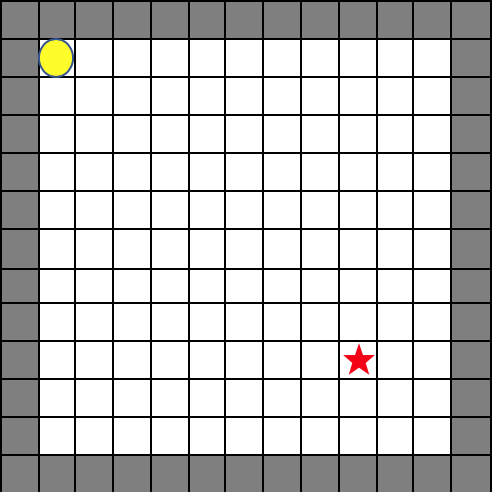
\includegraphics[width=\linewidth]{figures/chapter3/empty_room.png}
  ({a}) Empty Room         
\endminipage\hfill
\minipage{0.19\textwidth}
  \centering
  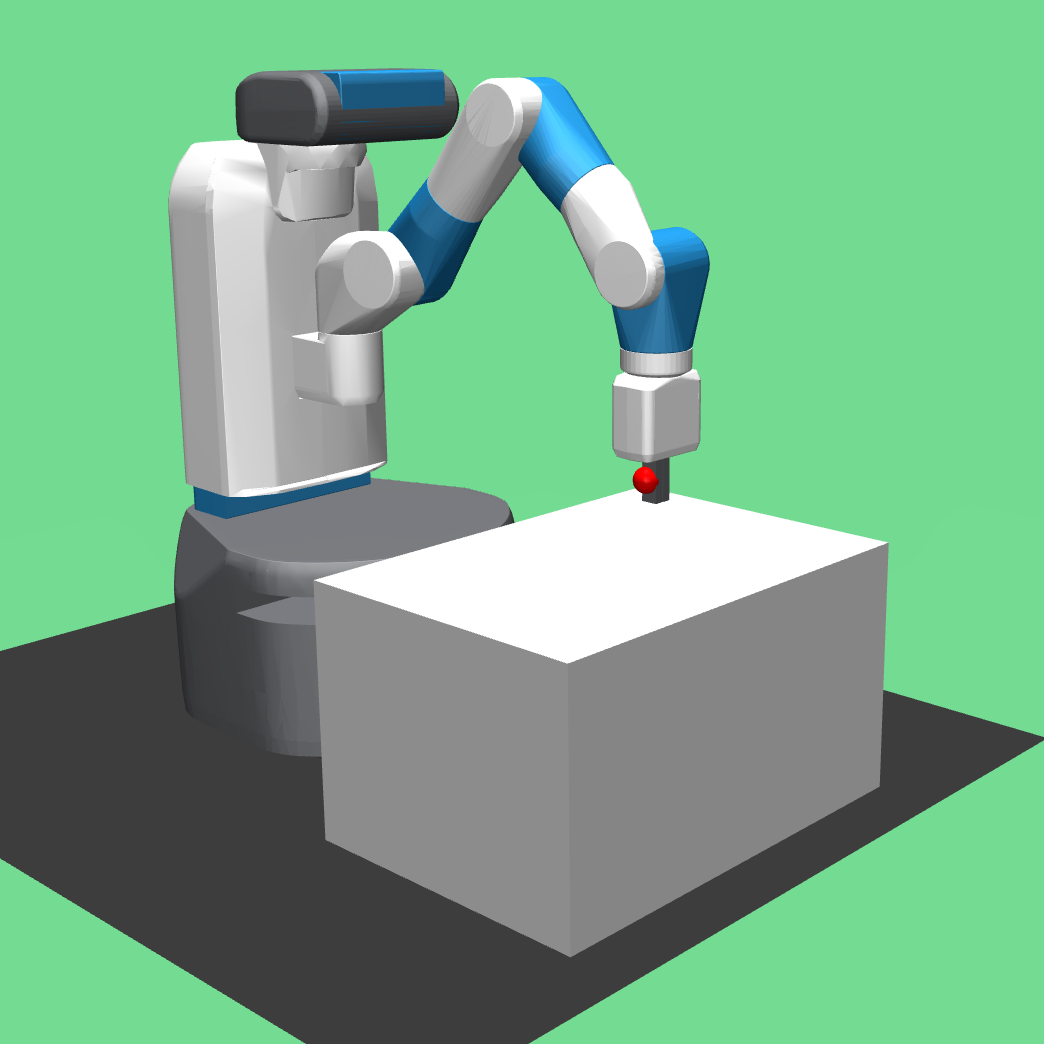
\includegraphics[width=\linewidth]{figures/chapter3/reach.png}
  ({b}) Reach 
\endminipage\hfill
\minipage{0.19\textwidth}%
  \centering
  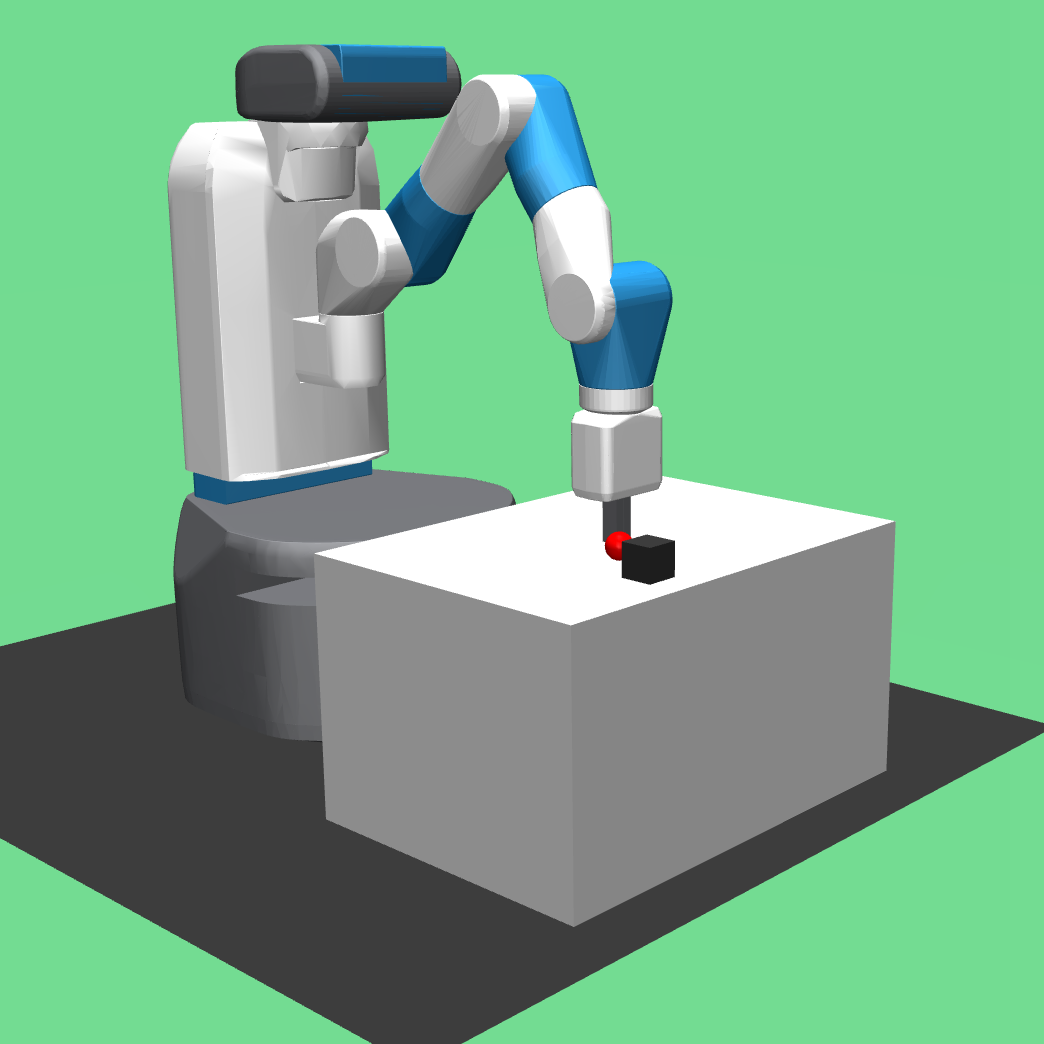
\includegraphics[width=\linewidth]{figures/chapter3/push.png}
  ({c}) Push      
\endminipage\hfill
\minipage{0.19\textwidth}%
  \centering
  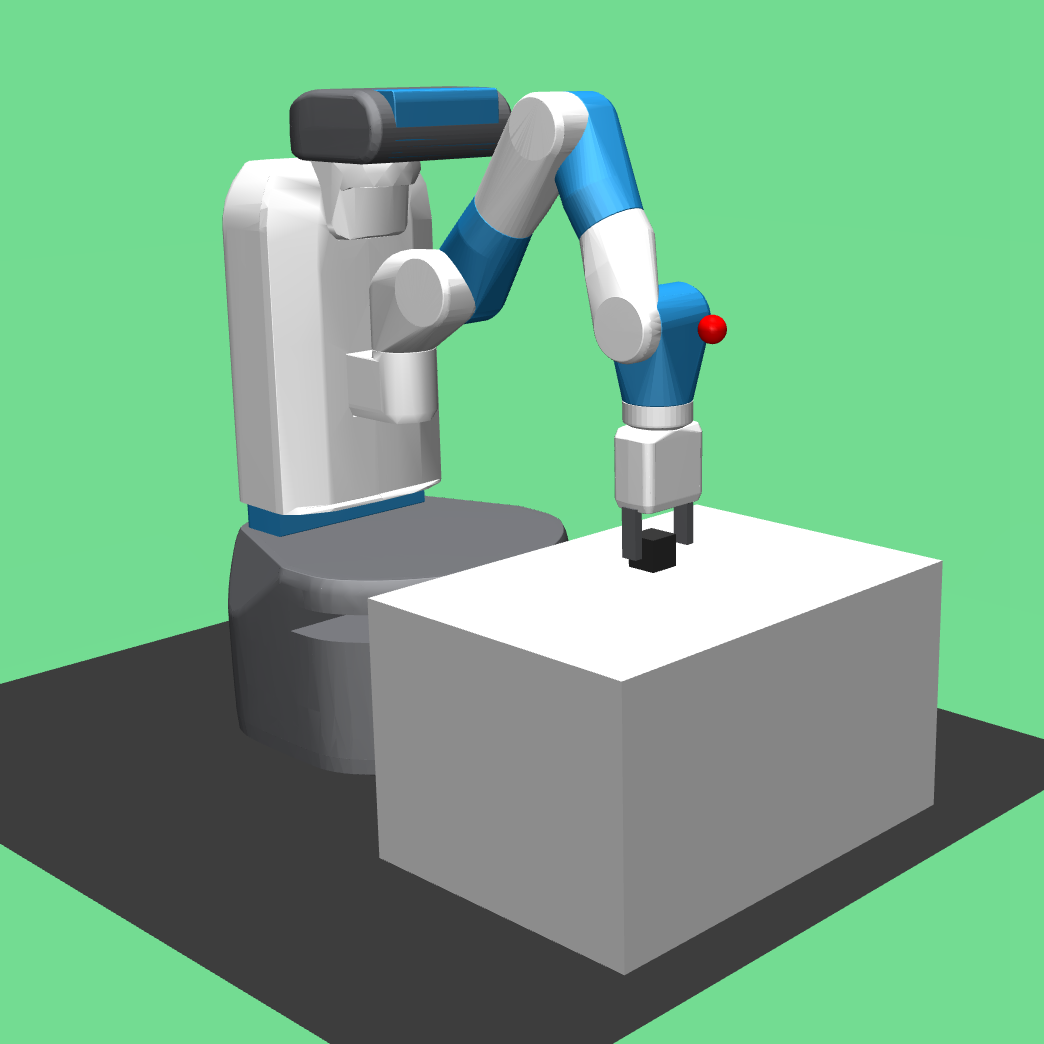
\includegraphics[width=\linewidth]{figures/chapter3/pick.png}
  ({d}) Pick$\&$Place
\endminipage\hfill
\minipage{0.19\textwidth}%
  \centering
  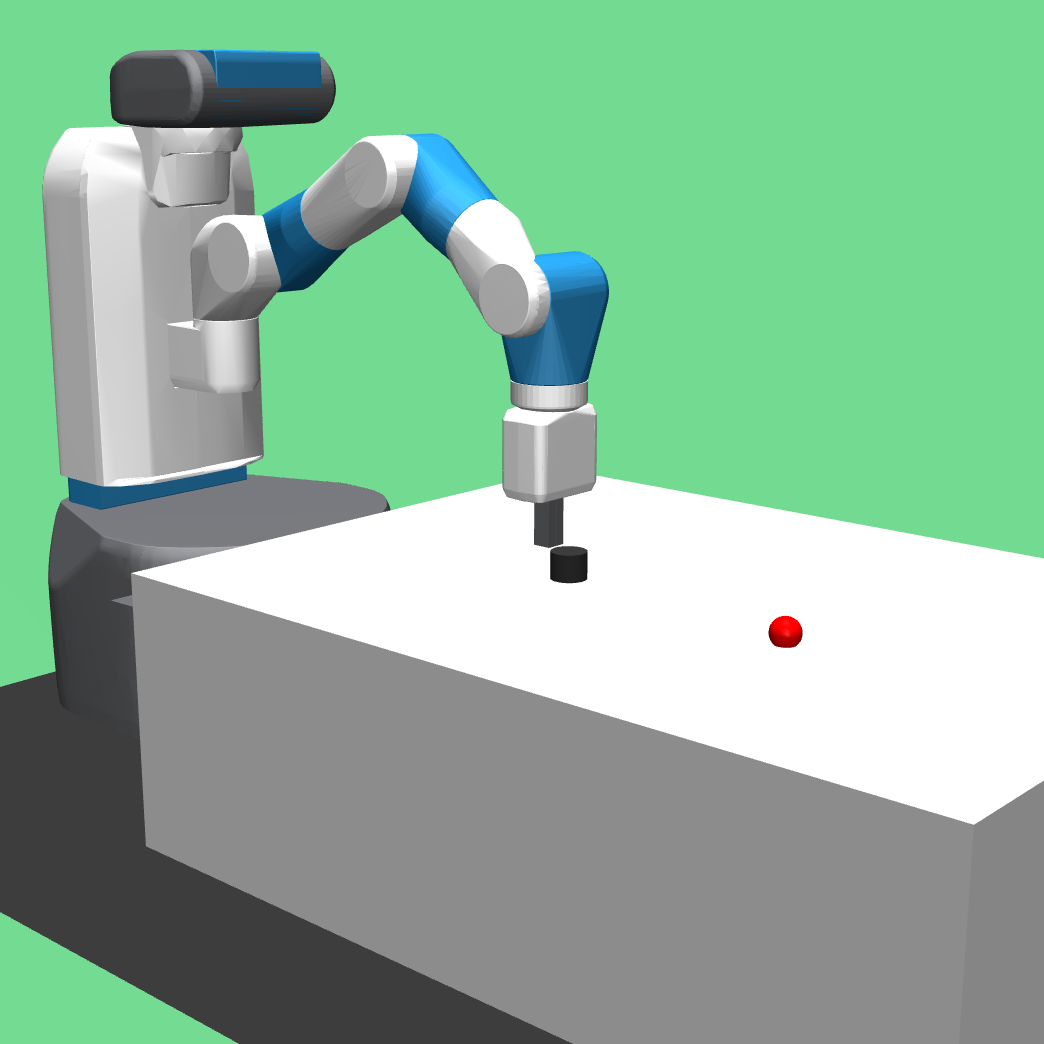
\includegraphics[width=\linewidth]{figures/chapter3/slide.png}
  ({e}) Slide     
\endminipage
\caption{Evaluation environments. ({a}) is the Empty Room environment, in which a yellow circle indicates the position of the agent and a red star represents a target position. ({b}--{e}) are the tasks in the Fetch robot environment. The red spot represents a target position.}
\label{fig:env}
\end{figure}

\subsection{Environments}
\textbf{{Empty Room (grid-world) environment}}:
The Empty Room environment is a simple grid-world environment. The agent is placed in an $11\times11$ grid, representing the room. The goal of the agent is to reach a target position in the room. The start position of the agent is at the left upper corner of the room, and the target position is randomly selected  within the room. When the agent chooses an action that would fall outside the grid area, the agent will stay at the current position. The length of each episode is 32. 
The desired goal, $g$, is a two-dimensional grid coordinate, which represents the target position. The achieved goal, $g^{ac}_{t}$, is also a two-dimensional coordinate, which represents the current position of the agent, and finally, the observation is a two-dimensional coordinate which represents the current position of the agent. 
The agent has five actions: left, right, up, down, and stay; the agent executes a random action with a probability of 0.2. The agent can get $+1$ as a reward only when $g^{ac}_{t+1}=g$, otherwise, it gets a reward of $0$. 

The agent is trained with 1 CPU core. In each epoch, 100 episodes are collected for the training. After each epoch, the agent is evaluated for 10 episodes. During training, the actions are sampled from the categorical distribution. During evaluation, the action with the highest probability will be chosen. 

\textbf{{Fetch robot (continuous) environment}%.
}~\cite{plappert2018multi}:~The Fetch robot environment is a physically plausible simulation based on the real Fetch robot. This environment aims to provide a platform to tackle problems that are close to practical challenging robot manipulation tasks. Fetch is a 7-DoF robot arm with a two-finger gripper. The Fetch environment include four~tasks: Reach, Push, Pick$\&$Place and Slide. For all Fetch tasks, the length of each episode is 50. The~desired goal, $g$, is a three-dimensional coordinate that represents the target position. If~a task has an object, the achieved goal $g^{ac}_{t}$ is a three-dimensional coordinate that represents the position of the object. Otherwise, $g^{ac}_{t}$ is a three-dimensional coordinate that represents the position of the gripper.
Observations include the following information: position, velocity, and state of the gripper. If a task has an object, the position, velocity, and rotation information of the object is included. Therefore, the~observation of the Reach task is a 10-dimensional vector.~The observation of other tasks is a 25-dimensional vector.~The~action is a four-dimensional vector. The first three dimensions represent the relative position the gripper needs to move in the next step. The last dimension indicates the distance between the fingers of the gripper.
The reward function can be written as $r_{t}=-\mathds{1}\left(\left\|g^{ac}_{t+1} - g\right\|>\epsilon\right)$, where $\epsilon =0.05$.

In the Fetch environment, for the Reach, Push, and Pick$\&$Place tasks, the agent is trained using 16 CPU cores. In each epoch, 50 episodes are collected for training. The Slide task is more complex than others, so 32 CPU cores are used. In each epoch, 100 episodes are collected for training. The~{message passing interface (MPI) framework is used to perform} synchronization when updating the network. After each epoch, the agent is evaluated for 10 episodes by each MPI worker. Finally,~the~success rate of each MPI worker is averaged. During training, the actions are sampled from {multivariate normal} distributions. In the evaluation phase, the mean value of the Gaussian distribution is used as an action. 

The proposed method, termed PPO+ESIL, is compared with different baselines in the different environments. All results are plotted based on five runs with different seeds. The solid line is the median value. The upper bound is the {75th} percentile, and the lower bound is the {25th} percentile.

\subsection{Experimental Settings}
\textbf{Network structure}: Both the actor network and the critic network have three hidden layers with 256~neurons. ReLU is selected as the activation function for the hidden layers. In the grid-world environment, the actor network builds a categorical distribution. In the Fetch environment, the actor network builds Gaussian {distribution by producing mean values and the standard deviations}.

\textbf{Hyperparameters}: For all experiments, the learning rate is 0.0003 for both the actor and critic networks. The discount factor $\gamma$ is 0.98. Adam is chosen as an optimiser. For each epoch, the~actor network and critic network are updated 10 times. The clip ratio of the PPO algorithm is 0.2. For the grid-world environment, networks are trained for 100 epochs with a batch size equal to 160. Each~epoch consists of 100 episodes. For the Fetch environment, in the Reach task, networks are trained for 100 epochs and other tasks for 1000 epochs with a batch size equals to 125. For the Reach, Push, and Pick$\&$Place tasks, each epoch consists of 50 episodes. For the Slide task, each epoch consists of 100 episodes. In designing the experiments, the number of episodes within an epoch is a balance between being able to train, the length of time required to run experiments and the maximum number of timesteps that would be required to achieve a goal. All environments have a fixed maximum number of timesteps, but this maximum differs depending on the problem or environment. This means that the number of state--action pairs can differ between two environments that have the same number of episodes and the same number of epochs. We arrange the episodes to try to compensate for the number of state--action pairs collected during training to make experiments easier to compare. The models are trained on a machine with an Intel i7-5960X CPU and 64GB RAM.

\begin{figure}[h!]
\minipage{0.5\textwidth}
  \centering
  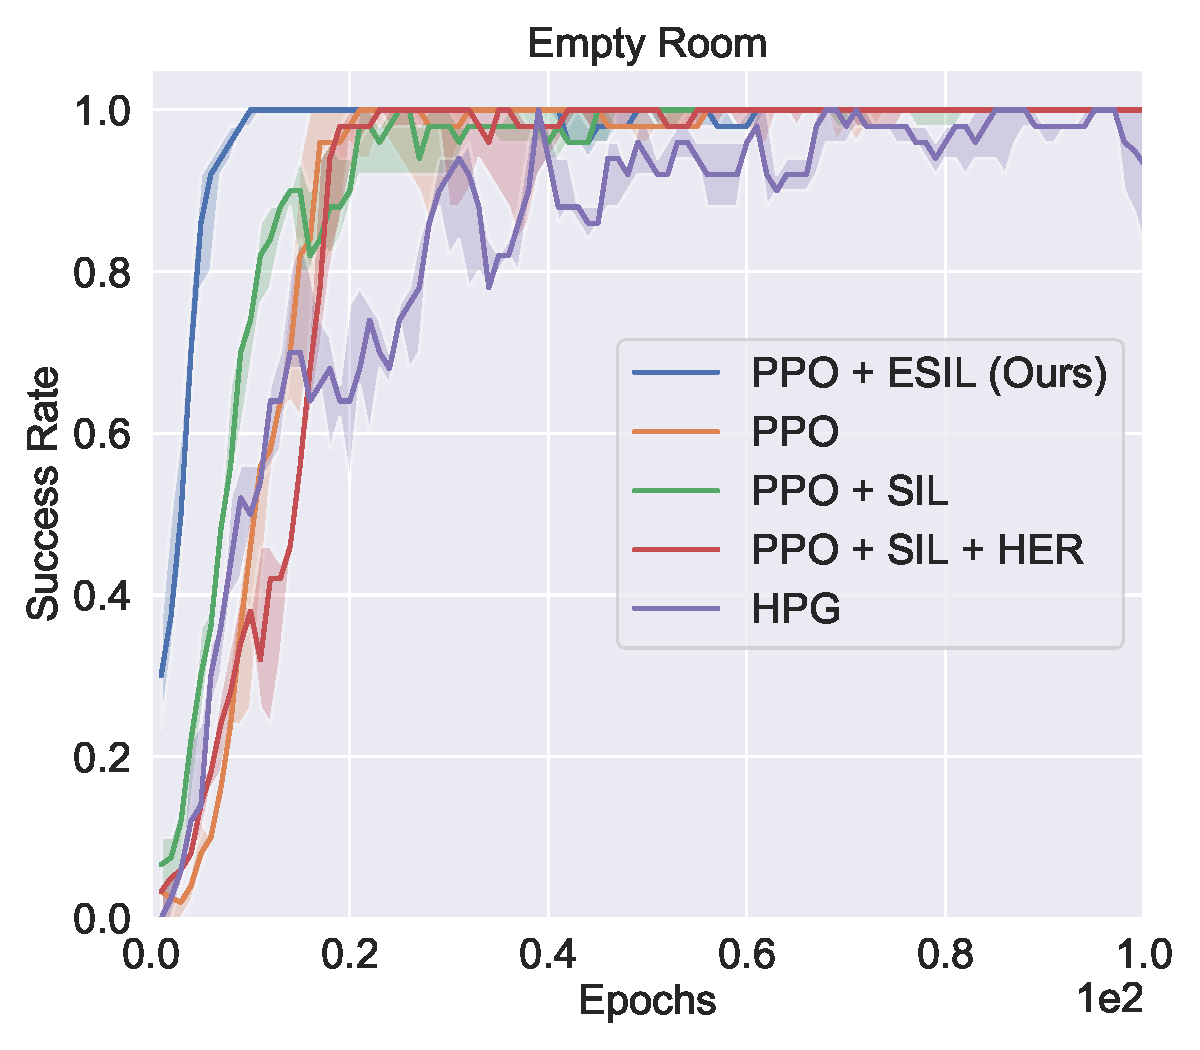
\includegraphics[width=\linewidth]{figures/chapter3/empty_room_baseline.pdf}
  ({a}) Comparison with on-policy baselines\hspace{3em} 
\endminipage
\minipage{0.5\textwidth}
  \centering
  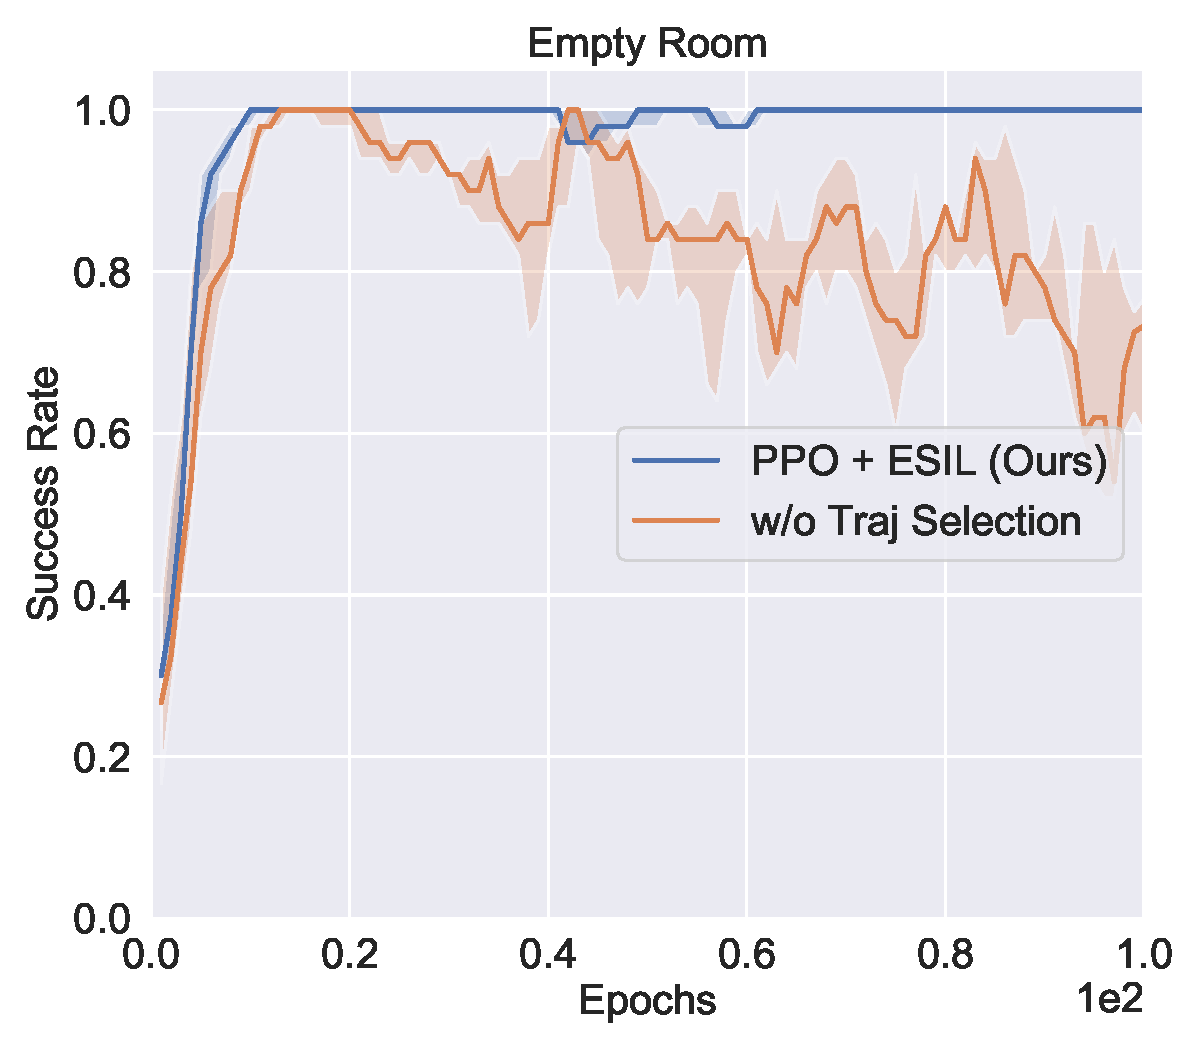
\includegraphics[width=\linewidth]{figures/chapter3/empty_room_hs.pdf}
  ({b}) {Ablation study of selection module}
\endminipage\hfill
\minipage{0.5\textwidth}%
  \centering
  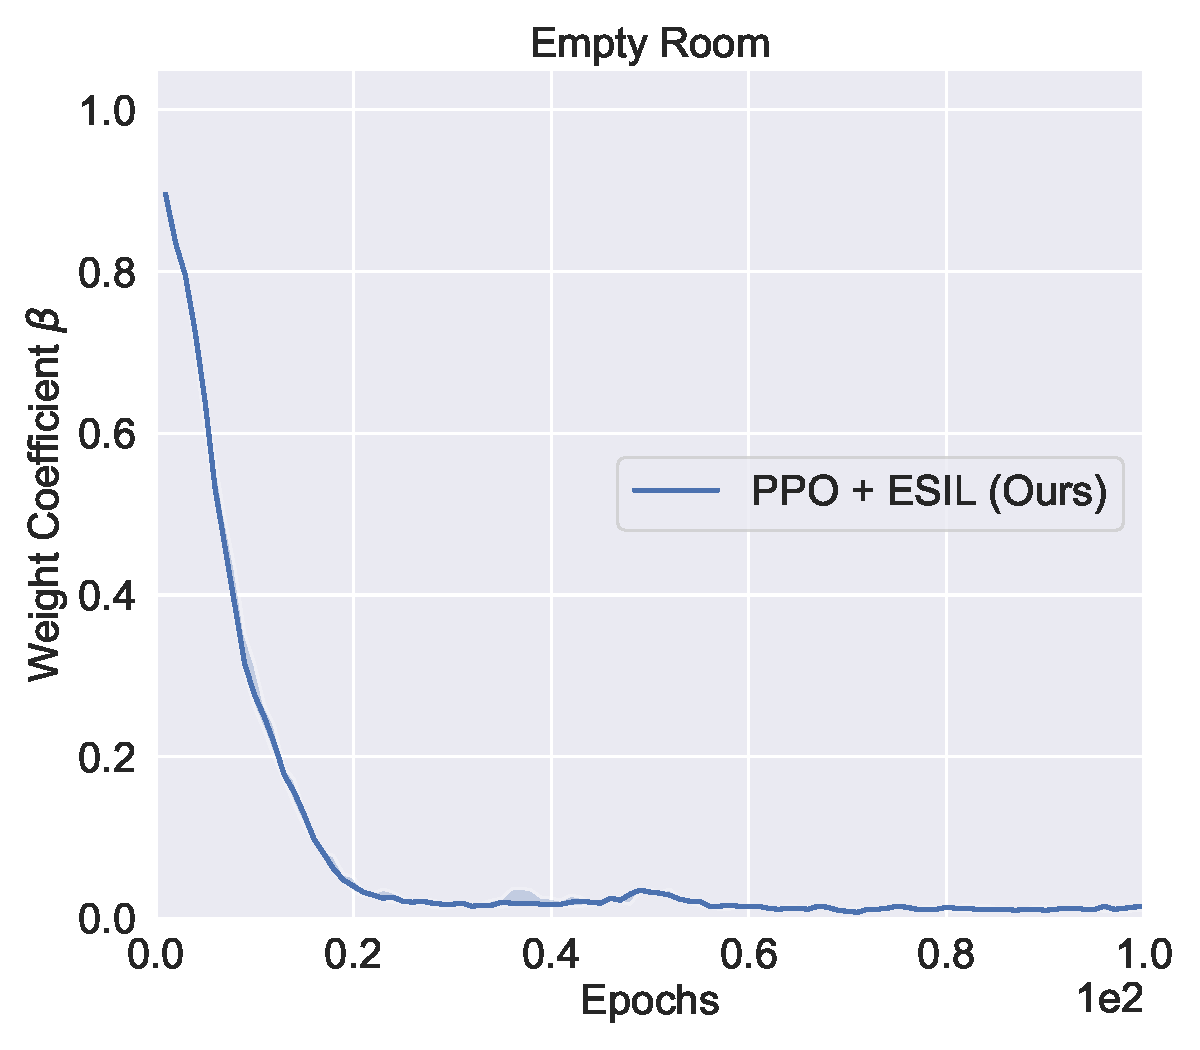
\includegraphics[width=\linewidth]{figures/chapter3/empty_room_samples.pdf}
  ({c}) Variation of adaptive weight $\beta$
\endminipage
\minipage{0.5\textwidth}%
  \centering
  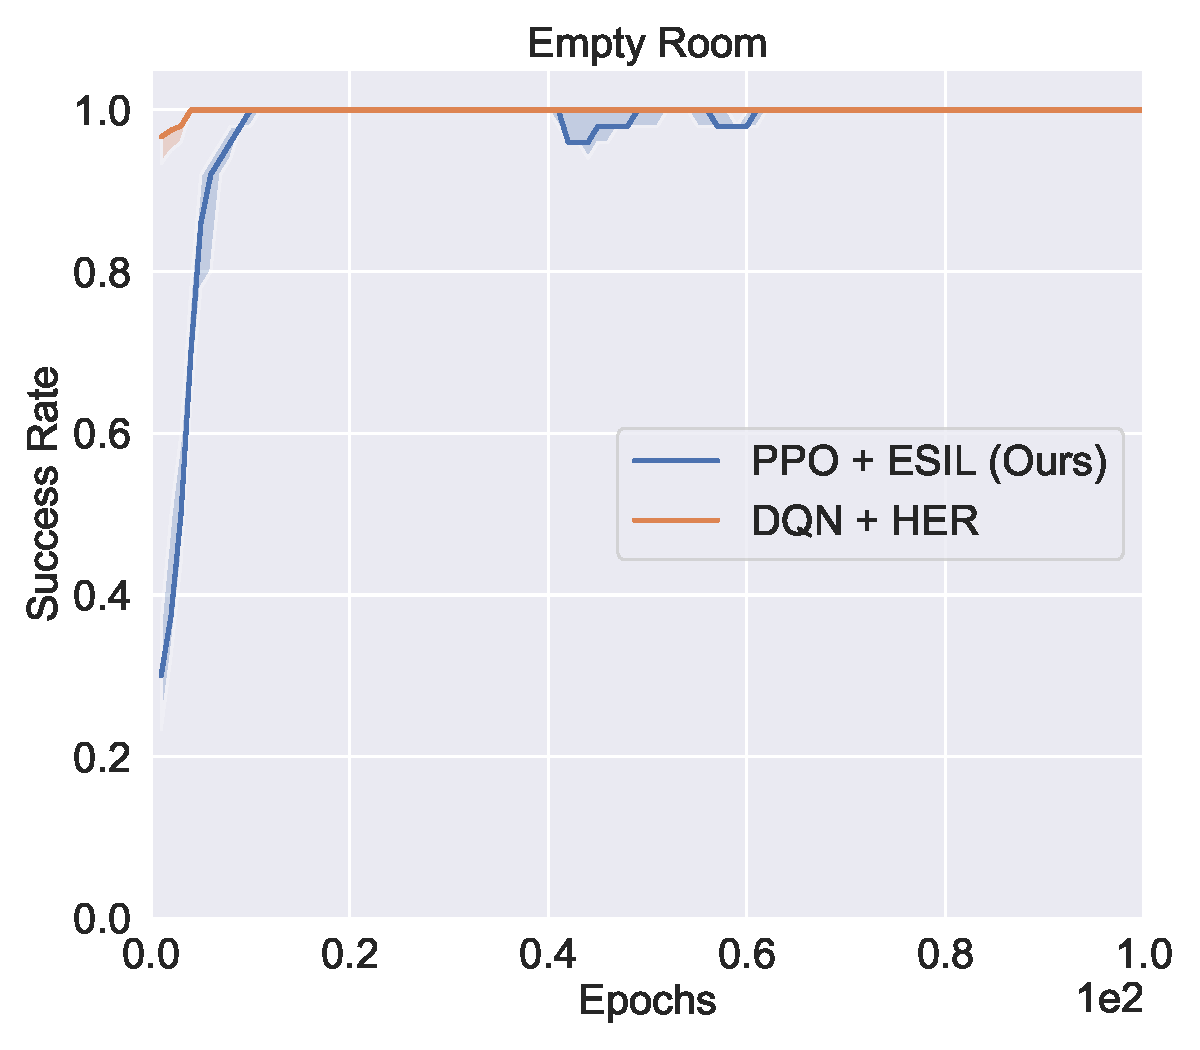
\includegraphics[width=\linewidth]{figures/chapter3/empty_room_her.pdf}
  ({d}) Comparison with off-policy baselines
\endminipage\hfill
\caption{Results of the grid-world environment. ({a}) Comparing the performance of PPO+ESIL between the on-policy approaches. ({b}) An ablation study on the trajectory selection module. ({c}) The variation of adaptive weight coefficient $\beta$ through training. ({d}) Comparison of the performance of PPO+ESIL to an off-policy approach: DQN+HER.}
\label{fig:toy_results}
\end{figure}

%\section{Results and Discussions}
\subsection{Results on Grid-World Environment}
To understand the basic properties of the proposed method, the toy Empty Room environment is used to evaluate ESIL.
%We compare the proposed method, named as PPO+HSL, with other baselines on the grid-world environment.
The following baselines are considered:
\begin{itemize}
    \item PPO: vanilla PPO~\cite{schulman2017proximal} for discrete action spaces;
    \item PPO+SIL/PPO+SIL+HER: Self-imitation learning (SIL) is used with PPO to solve hard exploration environments by imitating past good experiences~\cite{oh2018self}. In order to solve sparse rewards tasks, hindsight experience replay (HER) is applied to sampled transitions;
    \item DQN+HER: Hindsight experience replay (HER), designed for sparse reward problems, is~combined with a deep Q-learning network (DQN)~\cite{andrychowicz2017hindsight}; this is an off-policy algorithm;
    \item Hindsight Policy Gradients (HPG): the vanilla implementation of HPG that is only suitable for discrete action spaces~\cite{rauber2018hindsight}.
\end{itemize}
More specifically, {PPO+ESIL is compared with the above baseline methods} in Figure~\ref{fig:toy_results}a. This shows that PPO+ESIL converges faster than the other four baselines, and PPO+SIL converges faster than vanilla PPO, because PPO+SIL reuses past good experiences to help exploration and training. Hindsight policy gradient (HPG) is slower than the others because goal sampling is not efficient and is unstable. 

The performance of the trajectory selection module is evaluated in Figure~\ref{fig:toy_results}b. It shows that the selection strategy helps improve the performance. Hindsight experiences are not always perfect; the trajectory selection module filters some undesirable, modified experiences. Through adopting this selection strategy, the chance of agents learning from poor trajectories is reduced. The adaptive weight coefficient, $\beta$, is also investigated in these experiments. {In Figure~\ref{fig:toy_results}c, it can be seen that at the initial stages of training, $\beta$ is high}. {This is because, at this stage, the agent very seldom achieves the original goals}. The hindsight experiences can yield higher returns than the original experiences. {Therefore,~a~large proportion of hindsight experiences is selected to conduct self-imitation learning, helping the agent learn a policy for moving through the room}. In the later stages of training, the agent can achieve success frequently, and the hindsight experiences might be redundant (e.g., $G(s_{t}, g)\geq G(s_{t}, g^{\prime})$). In~this case, undesired hindsight experiences are removed by using the trajectory selection module and $\mathcal{L}_{PPO}$ leads the training. However, when the trajectory selection module is not employed, all hindsight experiences are used throughout the training, including the redundant hindsight experiences. This leads to overfitting and makes training unstable. Thus, $\mathcal{L}_{ESIL}$ can provide the agent with a better initial policy, and the adaptive weight coefficient $\beta$ can balance the contributions of $\mathcal{L}_{PPO}$ and $\mathcal{L}_{ESIL}$ properly during training.

Finally, {the combination of PPO+ESIL is also compared with DQN+HER,} which is an off-policy RL algorithm, in Figure~\ref{fig:toy_results}d. It shows that DQN+HER works a little better than ESIL at the {start of training}. However, the proposed method achieves similar results to DQN+HER later in training.

\subsection{Results on Continuous Control Environment}
% continuous control
{Continuous control problems are generally more challenging for reinforcement learning. In the experiments of this section, the aim is to investigate how useful the proposed method is for several hard exploration Fetch tasks. These robot manipulation tasks are commonly used to assess the performance of RL methods for continuous control.} The following baselines are considered: 
\begin{itemize}
    \item PPO: the vanilla PPO~\cite{schulman2017proximal} for continuous action spaces;
    \item PPO+SIL/PPO+SIL+HER: Self-imitation learning is used with PPO to solve hard exploration environments by imitating past good experiences~\cite{oh2018self}. For sparse rewards tasks, hindsight experience replay (HER) is applied to sampled transitions;
    \item DDPG+HER: this is the state-of-the-art off-policy RL algorithm for the Fetch tasks. Deep~deterministic policy gradient (DDPG) is trained with HER to deal with the sparse reward problem~\cite{andrychowicz2017hindsight}.
\end{itemize}

\begin{figure}[h!]
\centering
\minipage{0.5\textwidth}
  \centering
  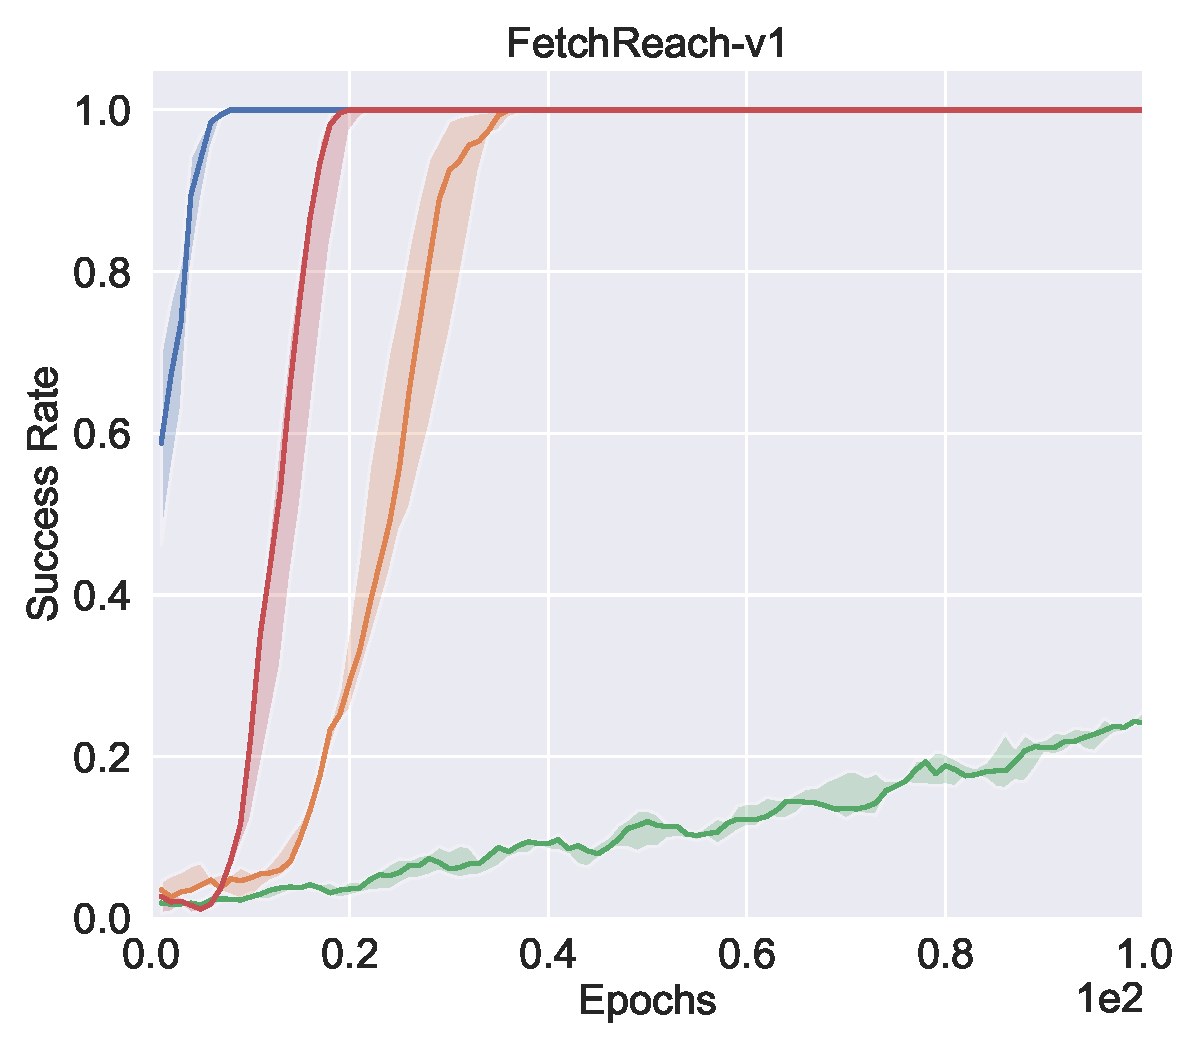
\includegraphics[width=\linewidth]{figures/chapter3/reach_baseline.pdf}
  ({a}) Reach
\endminipage
\minipage{0.5\textwidth}%
  \centering
  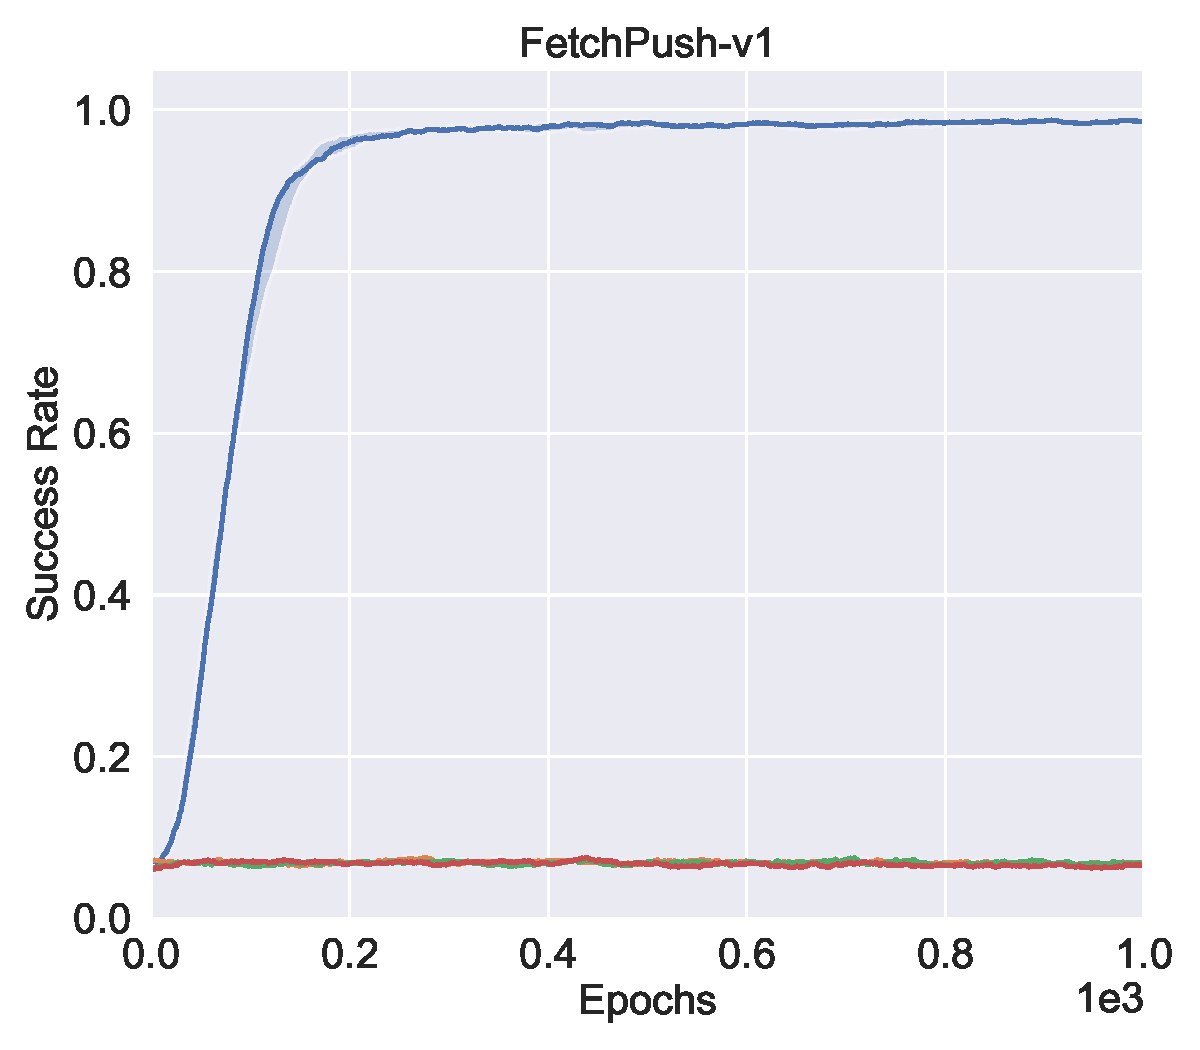
\includegraphics[width=\linewidth]{figures/chapter3/push_baseline.pdf}
  ({b}) Push
\endminipage\hfill
\minipage{0.5\textwidth}%
  \centering
  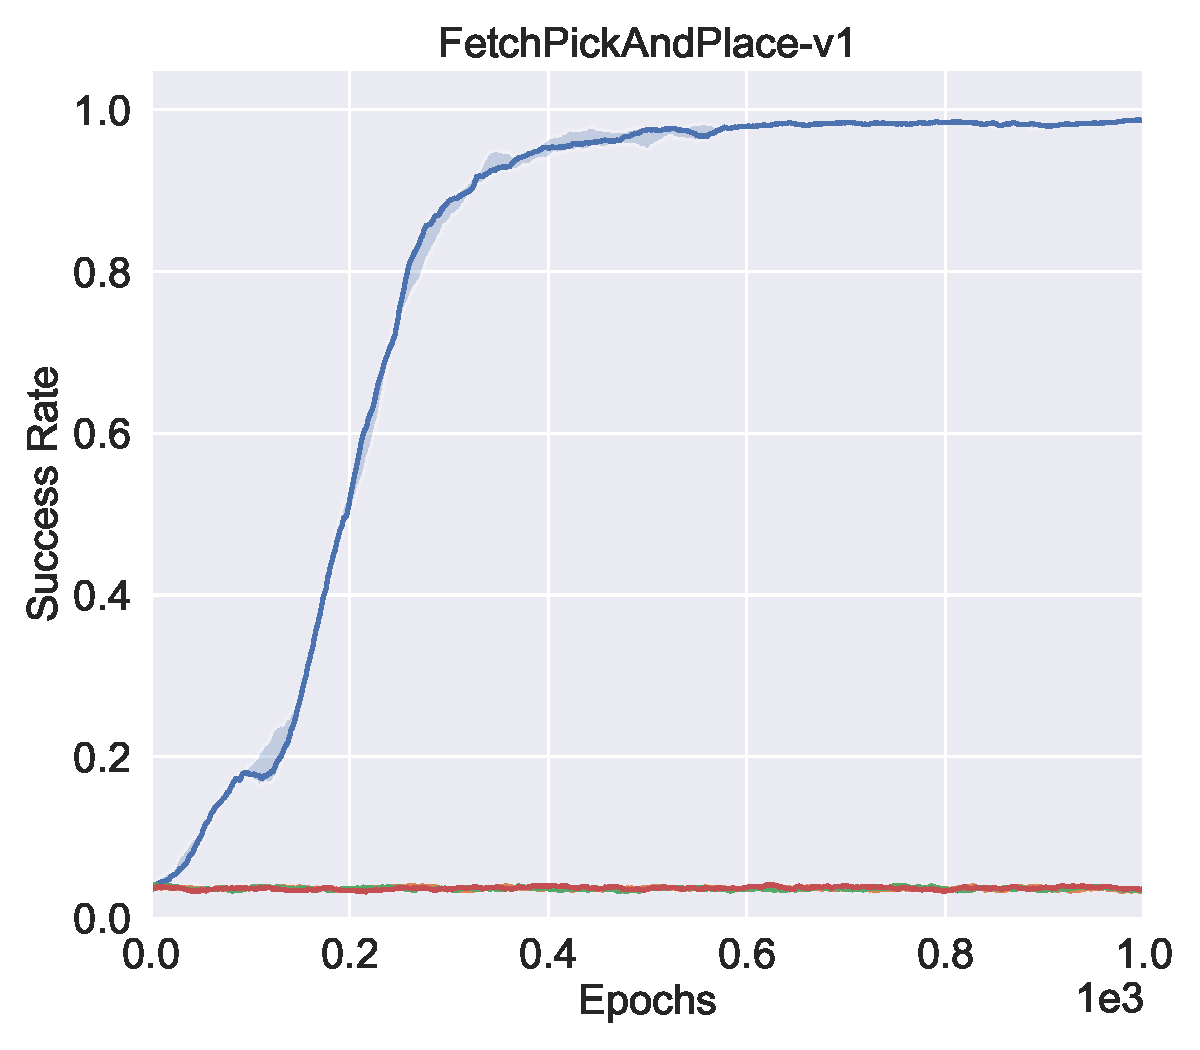
\includegraphics[width=\linewidth]{figures/chapter3/pick_baseline.pdf}
  ({c}) Pick$\&$Place
\endminipage
\minipage{0.5\textwidth}%
  \centering
  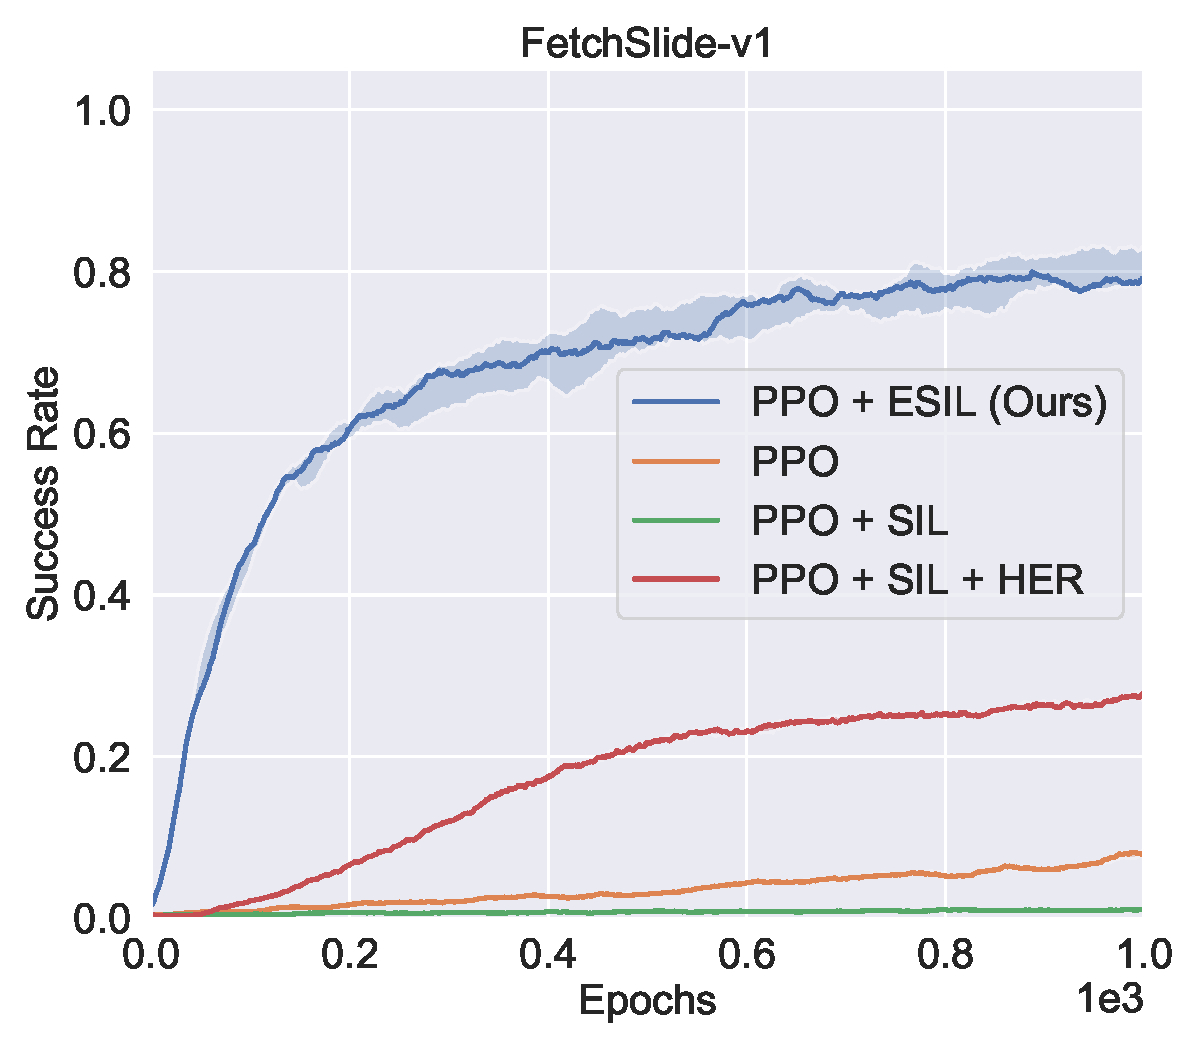
\includegraphics[width=\linewidth]{figures/chapter3/slide_baseline.pdf}
  ({d}) Slide
\endminipage\hfill
\caption{Results of comparison between ESIL and on-policy baselines in all Fetch tasks. \td{From the results, ESIL is able to resolve all of the tasks, while other baselines can only solve the simple Reach task.}}
\label{fig:baseline_compare}
\end{figure}

\subsubsection{Comparison to On-Policy Baselines}
{Figure~\ref{fig:baseline_compare}, PPO+ESIL} achieves reasonable results in all Fetch tasks. {In contrast}, PPO, PPO+SIL, and PPO+SIL+HER do not work in all tasks, except for the Reach task. In comparison with the other selected tasks from the Fetch environment, Reach task is relatively simple, because there is no object to be manipulated. For other tasks, it is quite difficult for the agent to achieve sufficient positive rewards during exploration, because of their rare occurrence. Although PPO+SIL utilises past good experiences to help exploration, it is still faced with the difficulty that past experiences do not easily achieve positive rewards. From the experiments ({see Figure~\ref{fig:baseline_compare}}), PPO+SIL (no hindsight) converges much more slowly than using PPO only. Attempting to use only the original trajectories for self-imitation learning leads to unsatisfactory performance. For PPO+SIL+HER (with no episodic update), the sampled transitions are modified into hindsight experiences, achieving better performance in the Reach and Slide tasks. However, this transition-based method still cannot solve the other two manipulation tasks. In contrast, the proposed PPO+ESIL, utilising episodic hindsight experiences from failed trajectories, can quickly achieve positive rewards at the start of~training.

\begin{figure}[h!]
\centering
\minipage{0.5\textwidth}
  \centering
  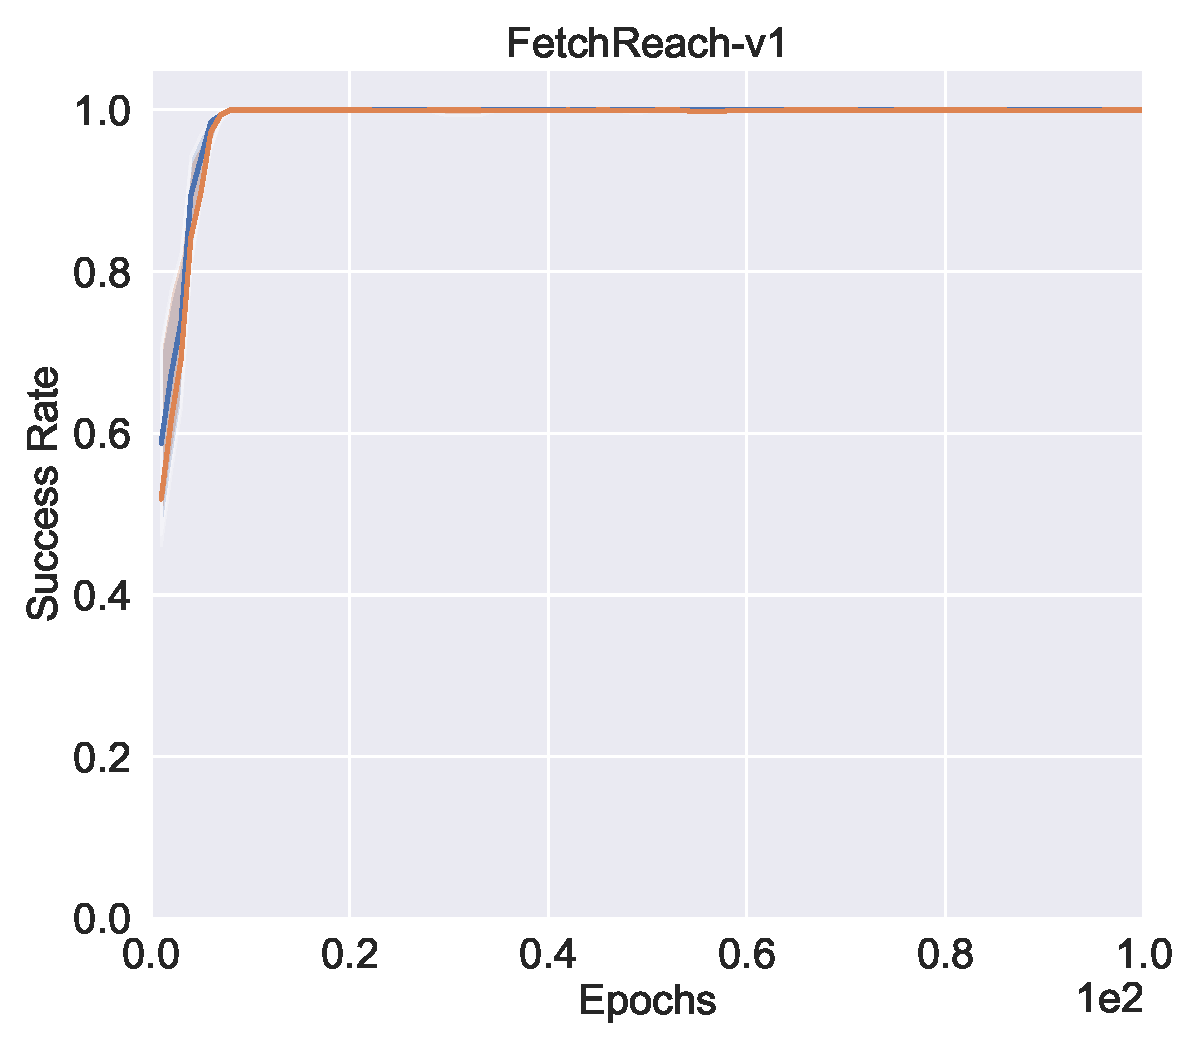
\includegraphics[width=\linewidth]{figures/chapter3/reach_hs.pdf}
  ({a}) Reach
\endminipage
\minipage{0.5\textwidth}%
  \centering
  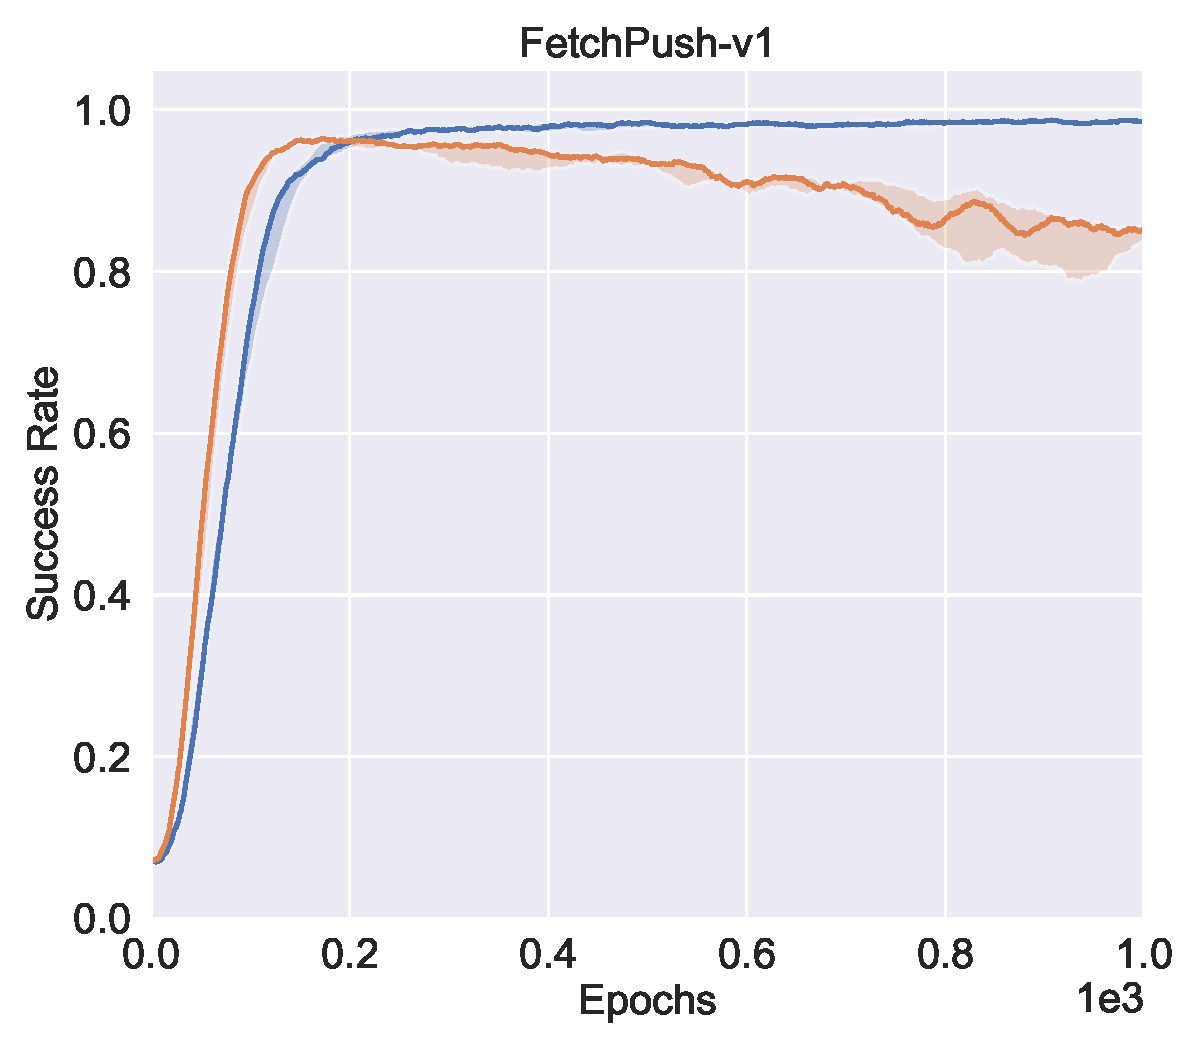
\includegraphics[width=\linewidth]{figures/chapter3/push_hs.pdf}
  ({b}) Push
\endminipage\hfill
\minipage{0.5\textwidth}%
  \centering
  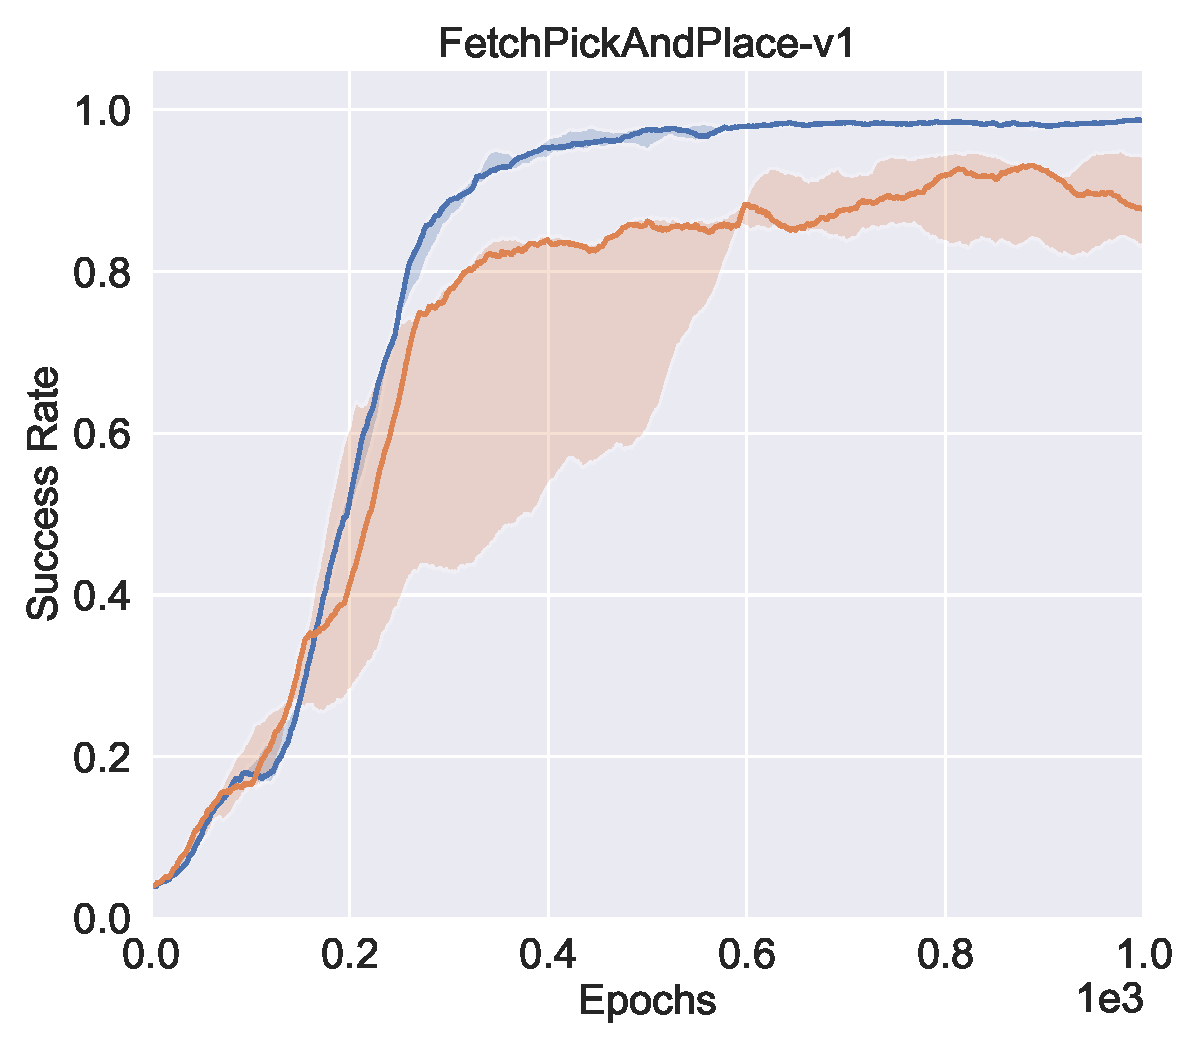
\includegraphics[width=\linewidth]{figures/chapter3/pick_hs.pdf}
  ({c}) Pick$\&$Place
\endminipage
\minipage{0.5\textwidth}%
  \centering
  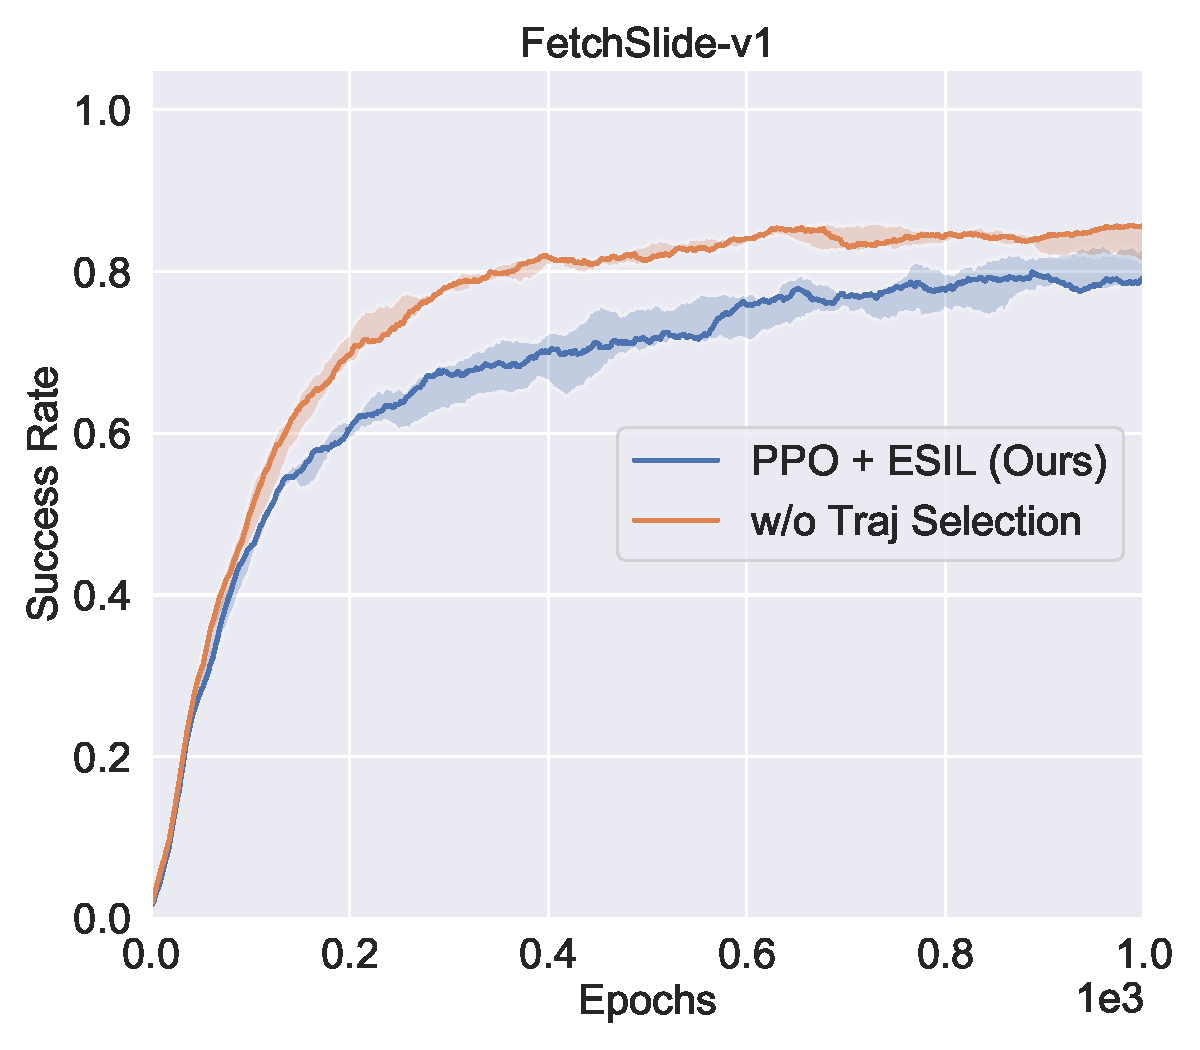
\includegraphics[width=\linewidth]{figures/chapter3/slide_hs.pdf}
  ({d}) Slide
\endminipage\hfill
\caption{Results of ablation studies with and without using the trajectory selection module in all Fetch tasks. \td{In three challenging tasks: Push, Pick$\&$Place and Slide, the trajectory selection module can stabilise the training and prevent performance degradation in two of three cases (Push and Pick$\&$Place).}}
\label{fig:hs_compare}
\end{figure}

\begin{figure}[h!]
\centering
\minipage{0.5\textwidth}
  \centering
  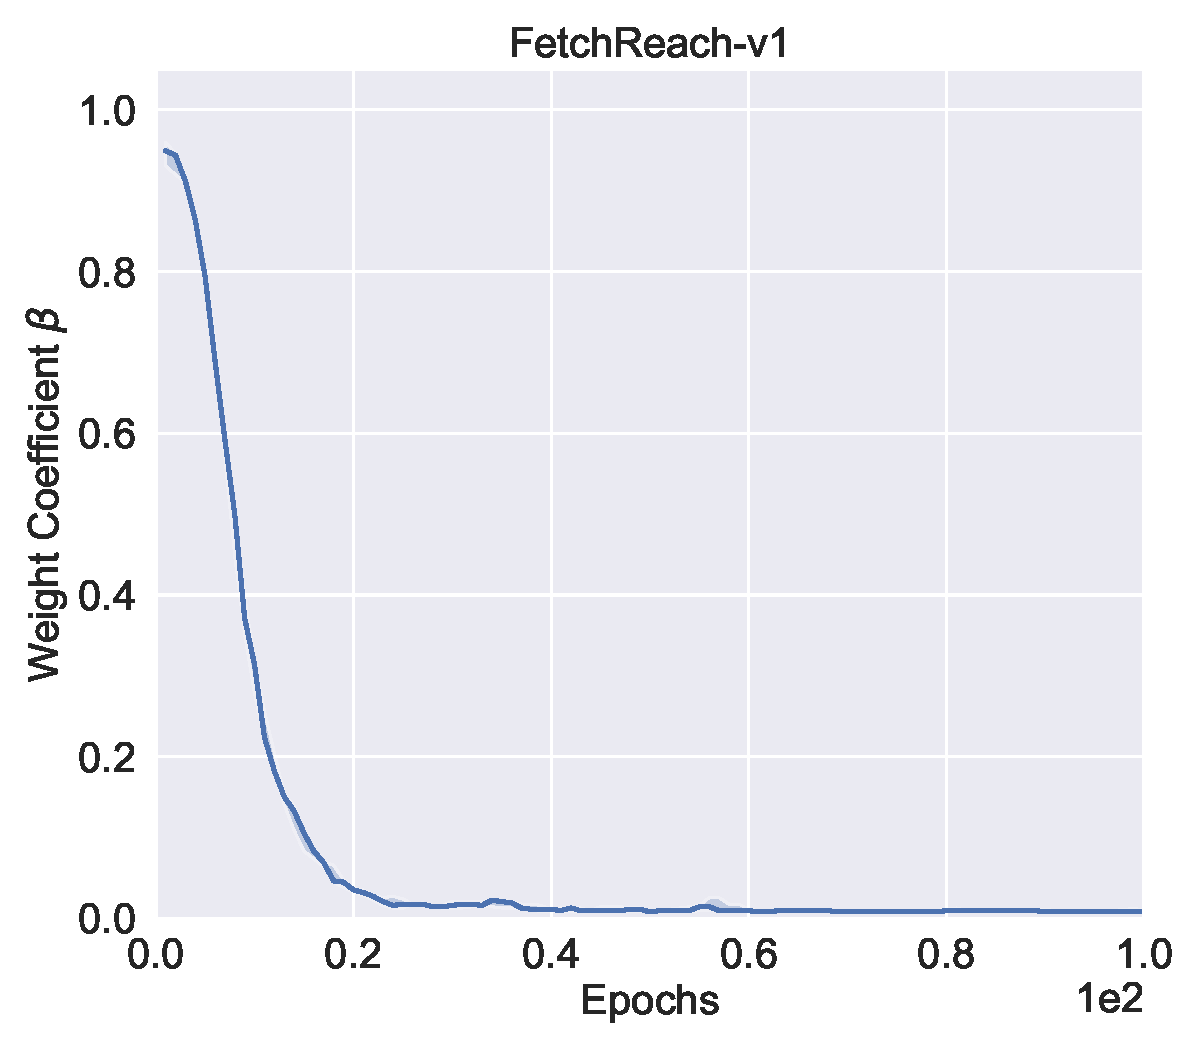
\includegraphics[width=\linewidth]{figures/chapter3/reach_samples.pdf}
  ({a}) Reach
\endminipage
\minipage{0.5\textwidth}%
  \centering
  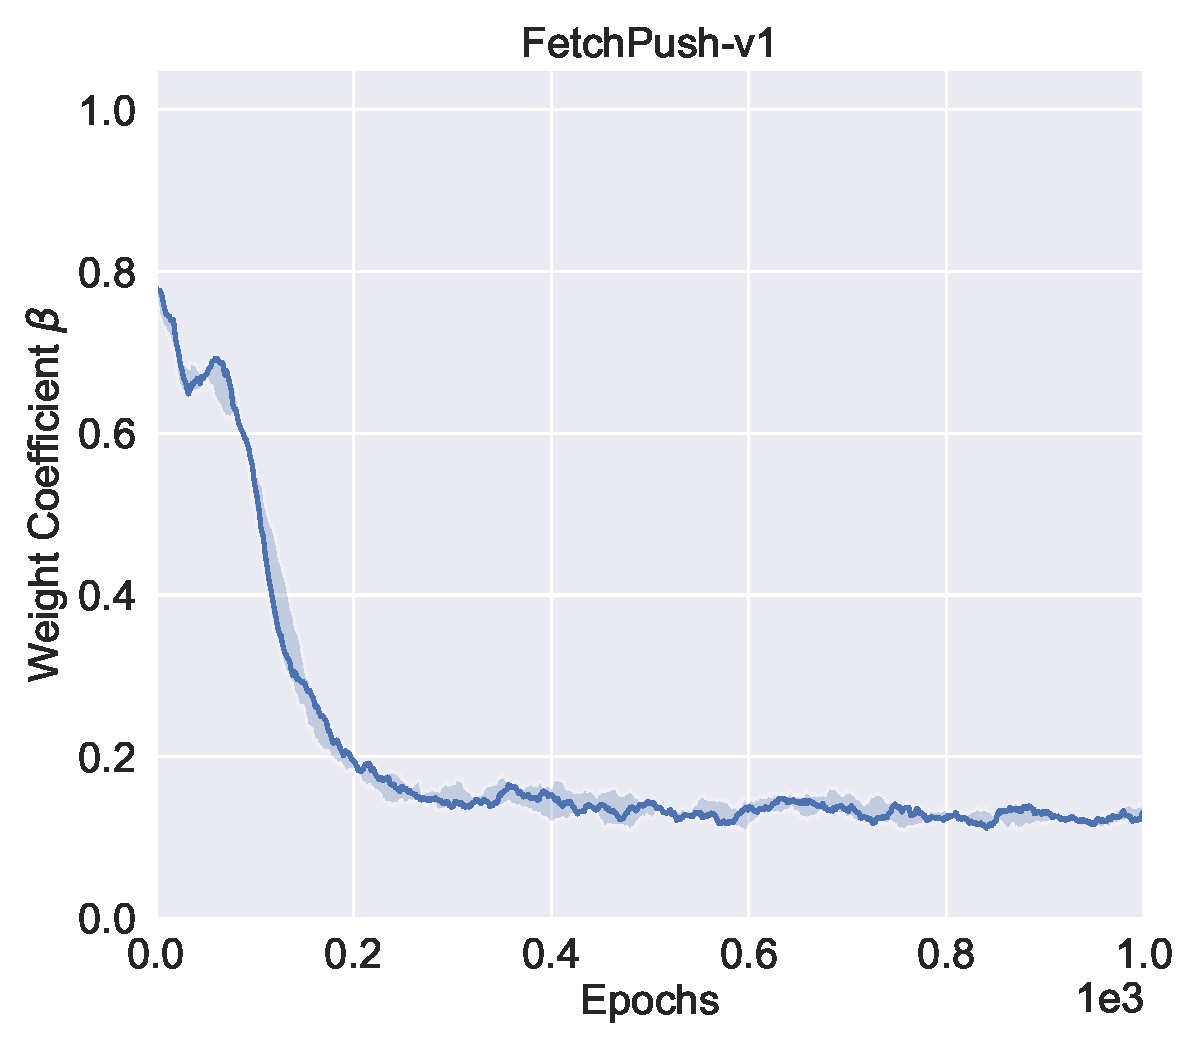
\includegraphics[width=\linewidth]{figures/chapter3/push_samples.pdf}
  ({b}) Push
\endminipage\hfill
\minipage{0.5\textwidth}%
  \centering
  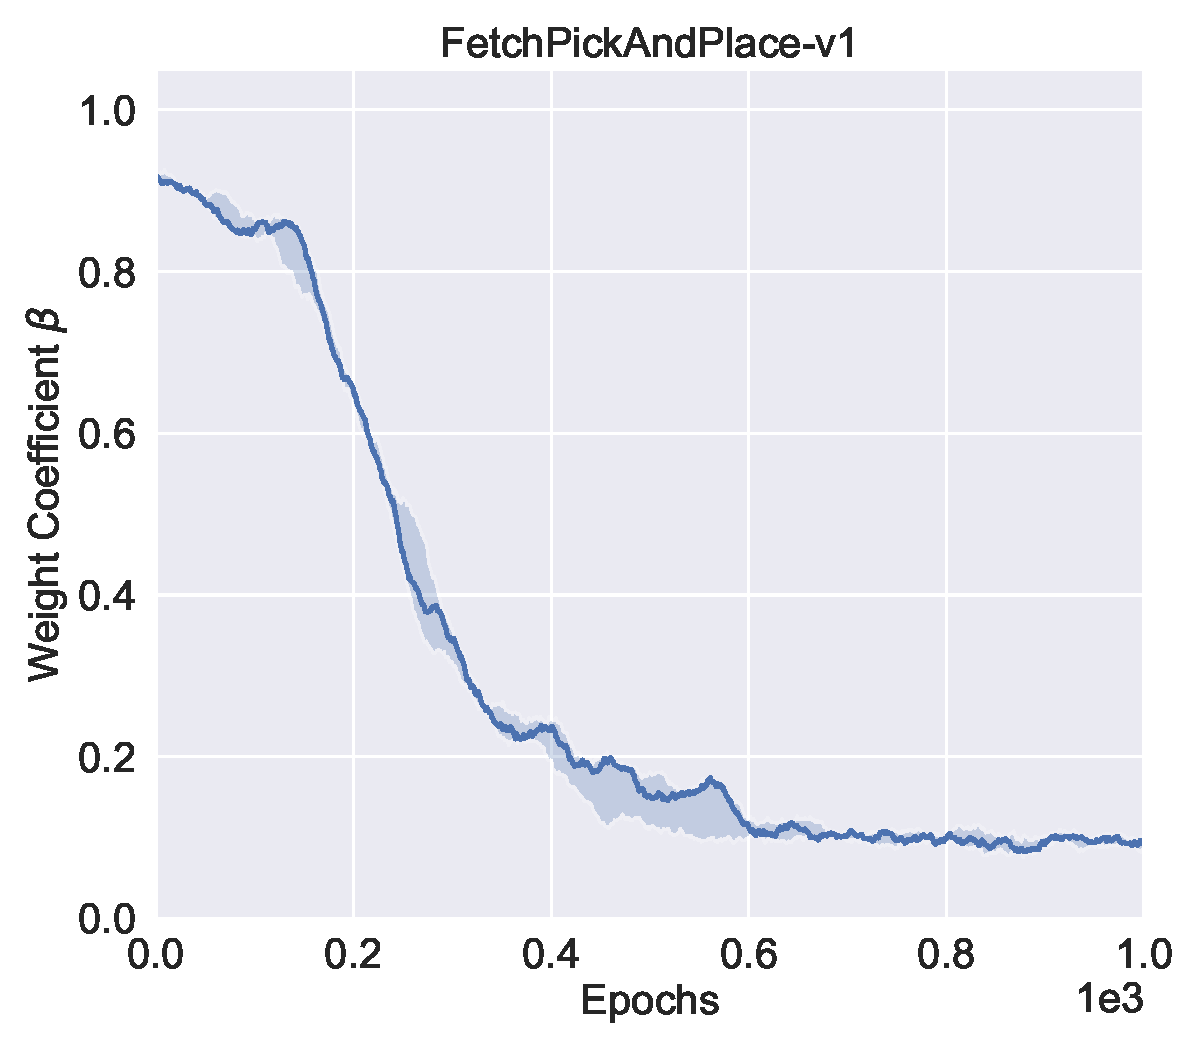
\includegraphics[width=\linewidth]{figures/chapter3/pick_samples.pdf}
  ({c}) Pick$\&$Place
\endminipage
\minipage{0.5\textwidth}%
  \centering
  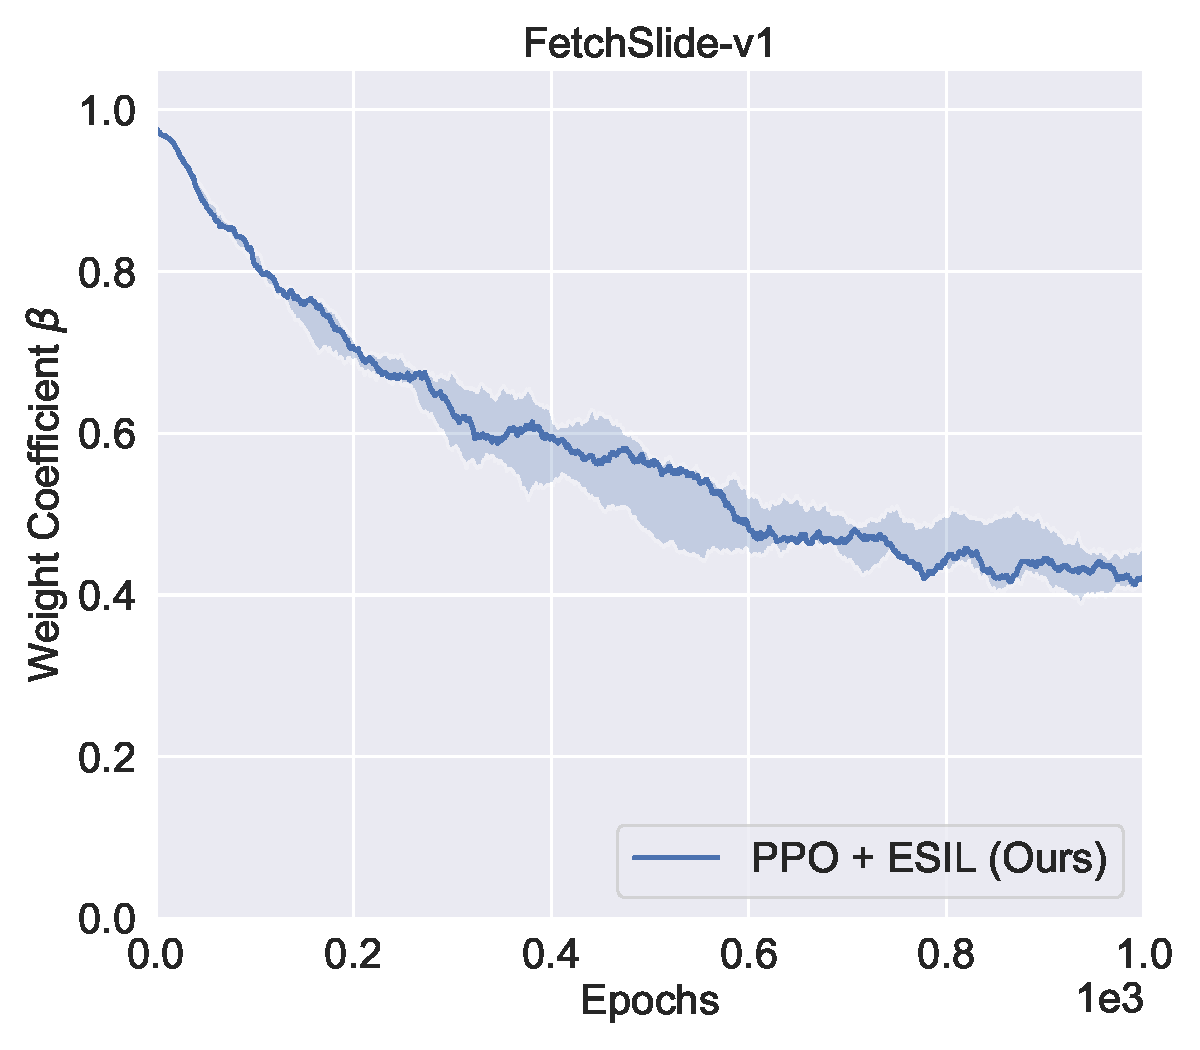
\includegraphics[width=\linewidth]{figures/chapter3/slide_samples.pdf}
  ({d}) Slide
\endminipage\hfill
\caption{Variation in adaptive weight coefficient $\beta$ through the training in all Fetch tasks. \td{In the early stage of training, the weight of the ESIL term is higher, which indicates more samples need to be modified to facilitate the exploration. As training progresses, the weight decreases, which means that the agent can achieve more positive samples and less modified samples are required.}}
\label{fig:her_samples_compare}
\end{figure}

\subsubsection{Ablation Study of Trajectory Selection Module}
To investigate the effect of trajectory selection, {ablation studies are performed} to validate the selection strategy of our approach. {Figure~\ref{fig:hs_compare}}, when the trajectory selection module is not used, the~ performance of the agent increases at first, and then starts to decrease. This suggests that the agent starts to converge to a sub-optimal location. However, {Figure~\ref{fig:hs_compare}d}, for the Slide task, the agent converges faster without the trajectory selection module and has better performance. {This is likely to be because the Slide task is the most difficult of the Fetch environment. During training, the agent is unlikely to achieve positive rewards. Figure~\ref{fig:her_samples_compare} also indicates that the value of $\beta$ in the Slide task is higher than values in other tasks, which means the majority of hindsight experiences have higher returns than original experiences. Thus, using {\em more} hindsight experiences (without filtering) accelerates training at this stage.} Nonetheless, the trajectory selection module prevents the agent from overfitting the hindsight experience in the other three tasks. Figure~\ref{fig:her_samples_compare}, shows the adaptive weight coefficient $\beta$ in all Fetch tasks. When the trajectory selection module is used, the value of $\beta$ decreases with the increase in training epochs. This implies that the agent can achieve a greater proportion of the original goals in the latter stages of training, and fewer hindsight experiences are required for self-imitation learning.
\begin{figure}[h!]
\minipage{0.5\textwidth}
  \centering
  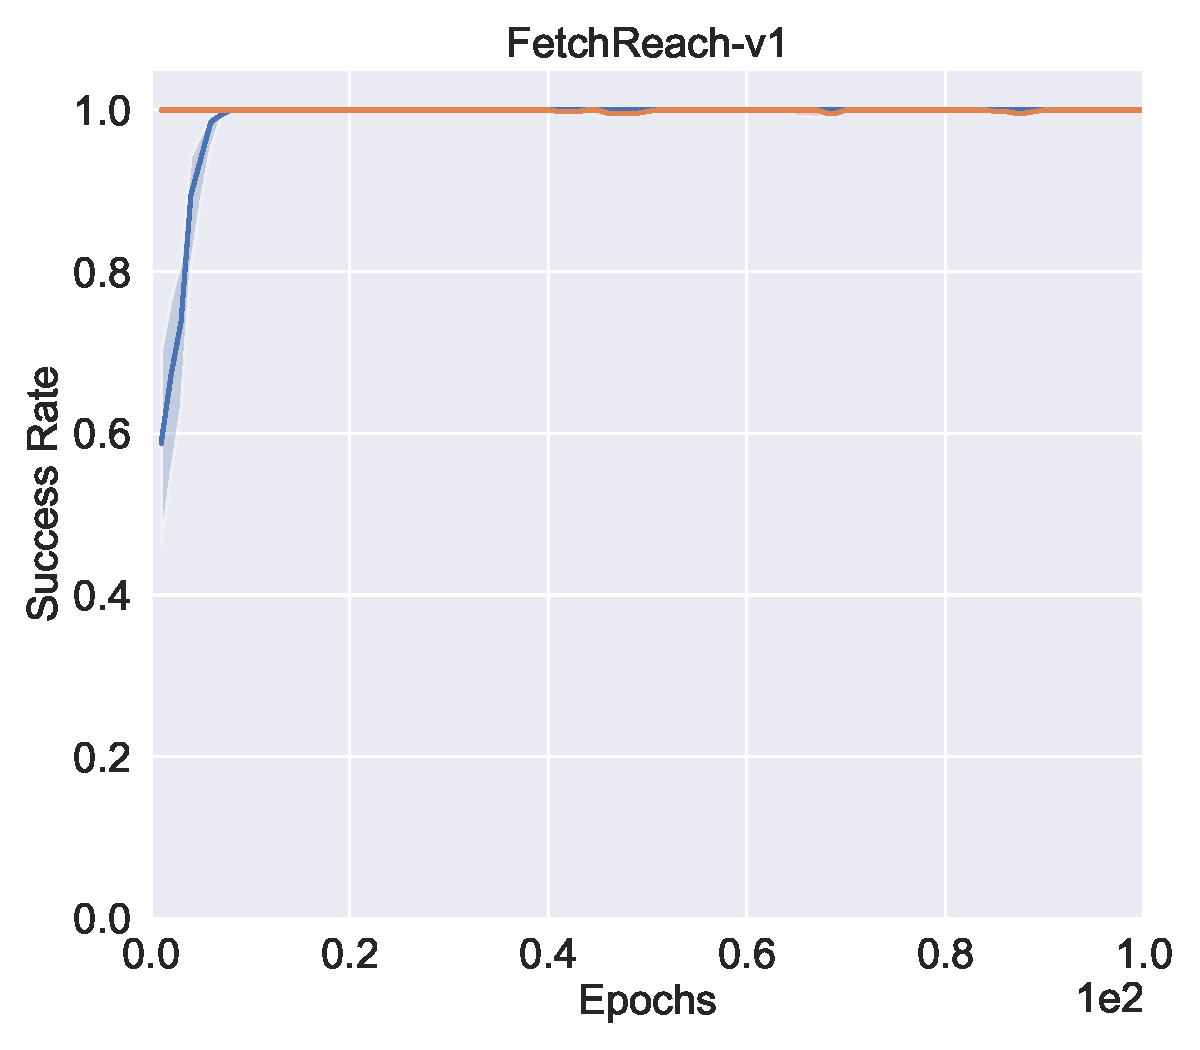
\includegraphics[width=\linewidth]{figures/chapter3/reach_her.pdf}
  ({a}) Reach
\endminipage
\minipage{0.5\textwidth}%
  \centering
  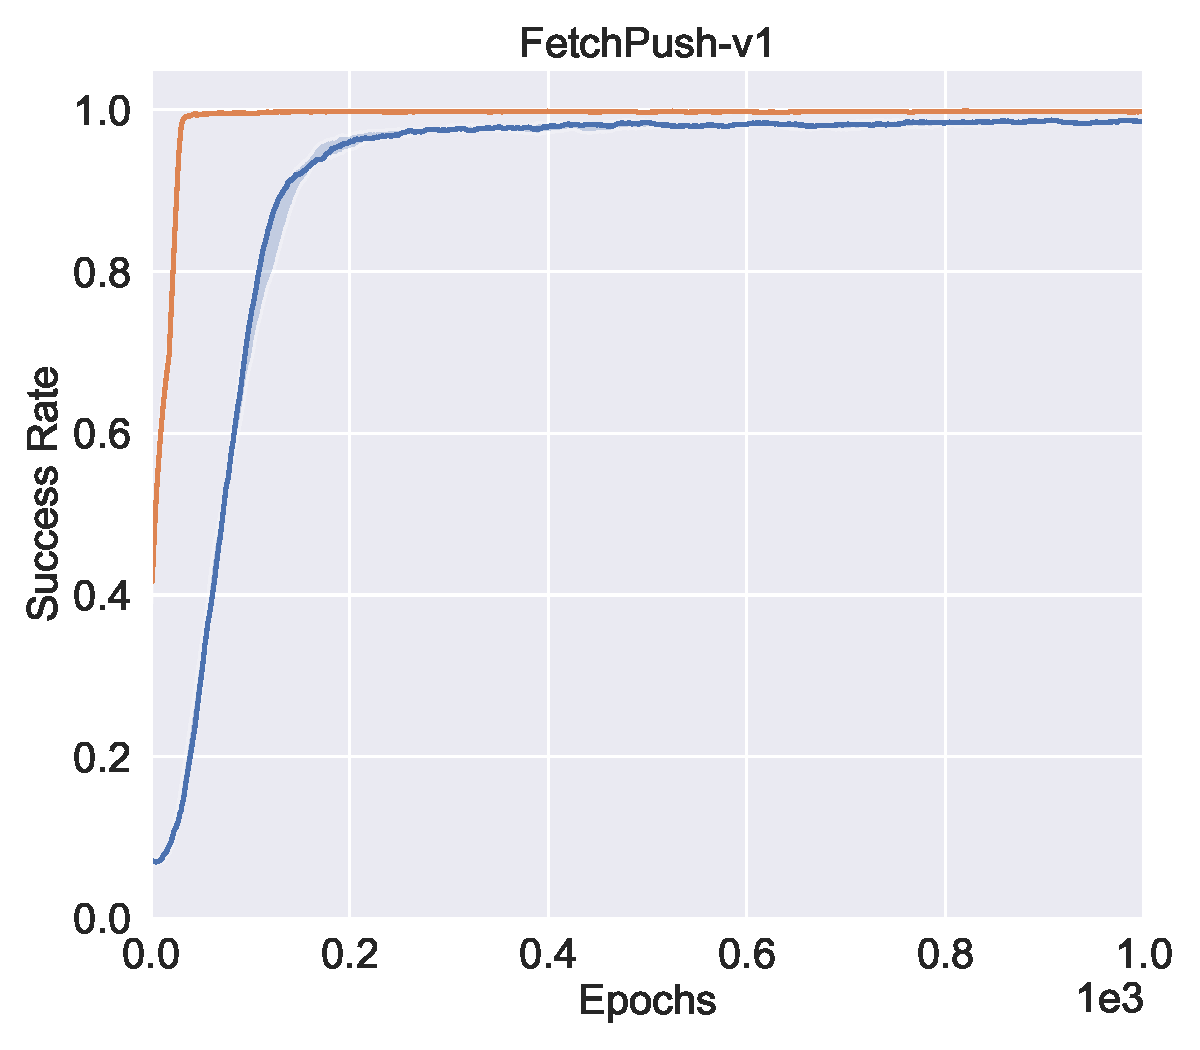
\includegraphics[width=\linewidth]{figures/chapter3/push_her.pdf}
  ({b}) Push
\endminipage\hfill
\minipage{0.5\textwidth}%
  \centering
  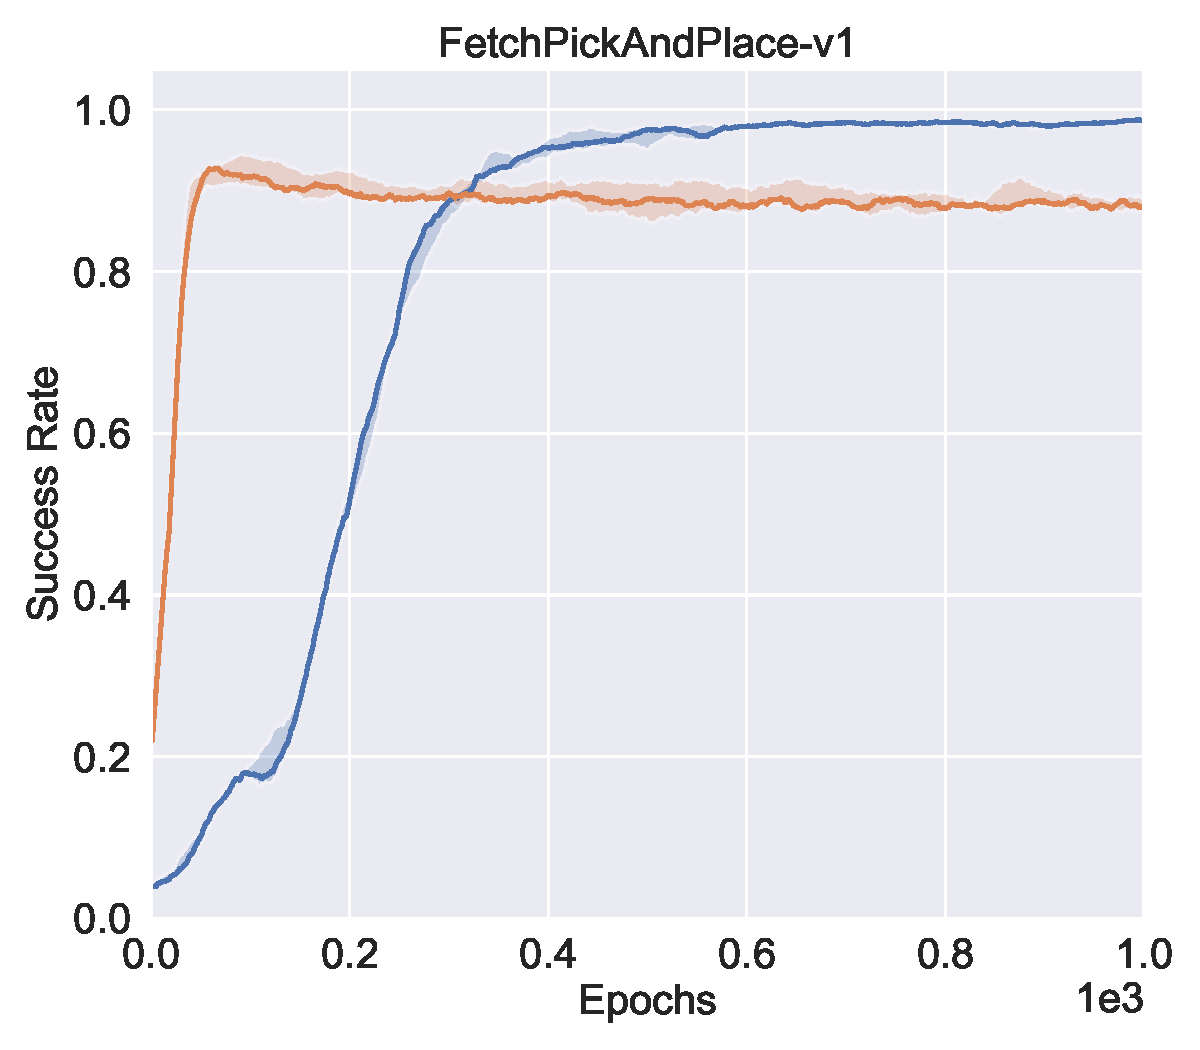
\includegraphics[width=\linewidth]{figures/chapter3/pick_her.pdf}
  ({c}) Pick$\&$Place
\endminipage
\minipage{0.5\textwidth}%
  \centering
  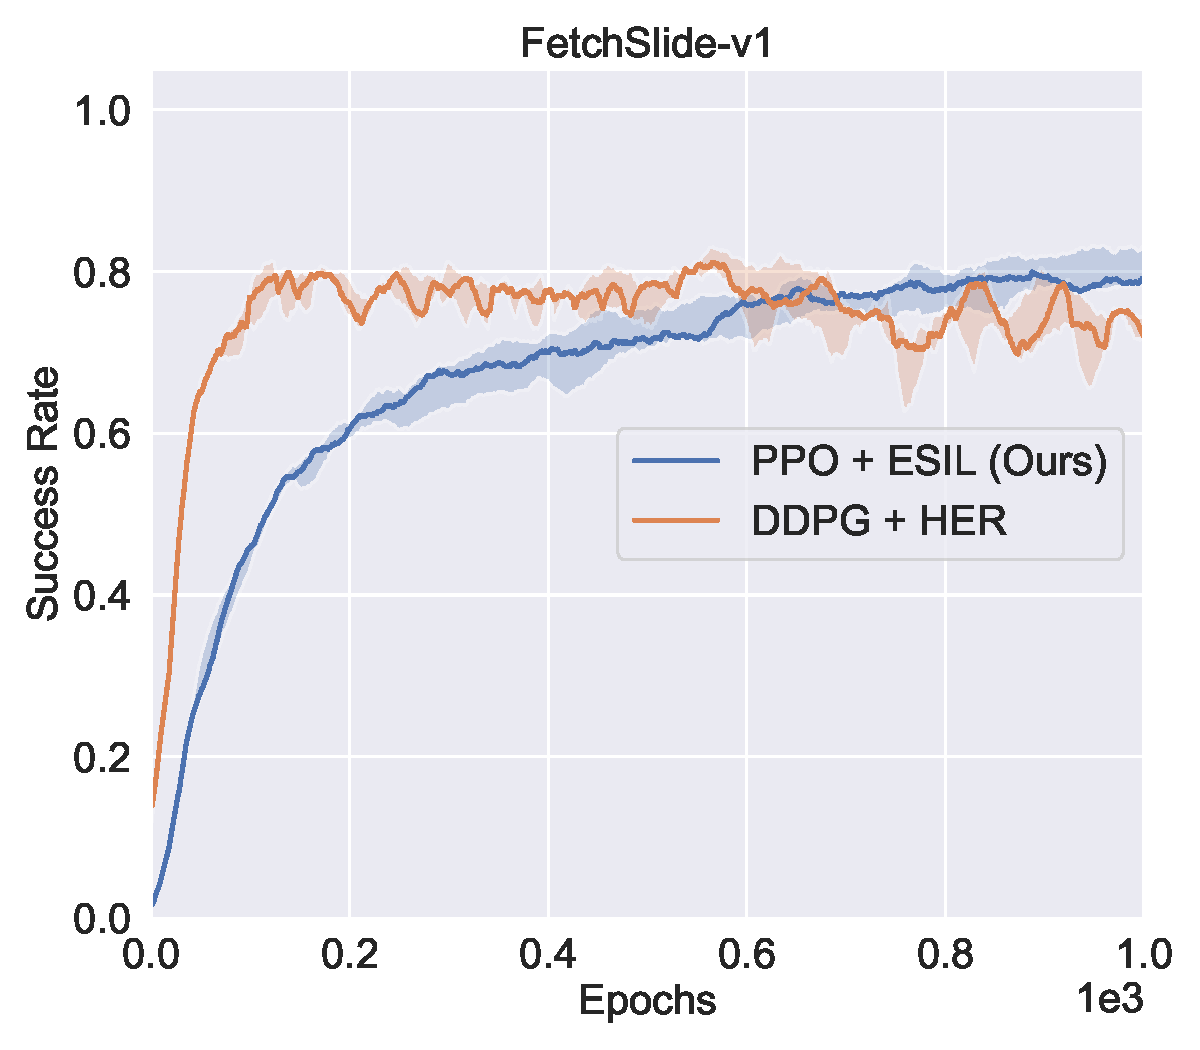
\includegraphics[width=\linewidth]{figures/chapter3/slide_her.pdf}
  ({d}) Slide
\endminipage\hfill
\caption{Results of the comparison between PPO+ESIL and DDPG+HER in all fetch tasks. \td{From the results, PPO+ESIL has worse sample efficiency than the off-policy baseline. However, PPO+ESIL achieves similar or even better performance in the end of training.}}
\label{fig:her_compare}
\end{figure}

\subsubsection{Comparison to Off-Policy Baselines}
Finally, {the proposed method is also compared} with a state-of-the-art off-policy algorithm: DDPG+HER. From {Figure~\ref{fig:her_compare}, it may be seen that} DDPG+HER converges faster than PPO+ESIL in all tasks. {However, PPO+ESIL obtains a similar performance to DDPG+HER. This is because DDPG+HER is an off-policy algorithm and uses a large number of hindsight experiences. A replay buffer is also employed to store  samples collected in the past. This approach has better sample efficiency than on-policy algorithms such as PPO.} Even so, {Figure~\ref{fig:her_compare}c} shows that PPO+ESIL still outperforms DDPG+HER in the Pick$\&$Place task and the success rate is close to 1. {This suggests that PPO+ESIL approximates the characteristics of on-policy algorithms, which have low sample efficiency, but are able to obtain a comparable performance to off-policy algorithms in continuous control tasks~\cite{schulman2017proximal}.}

\subsection{Overall Performance}
{Table~\ref{tb:ch3_last}} shows the average success rate of the last 10 epochs during training of baseline methods and PPO+ESIL. The proposed ESIL achieves the best performance in four out of five tasks. However,~PPO and PPO+SIL only obtain reasonable results in the Empty Room and Reach task. With the assistance of HER, PPO+SIL+HER obtains a better performance in the Slide task. {For the off-policy method of DDPG+HER, all five tasks are achieved, but it only obtain a better performance than PPO+ESIL in the Push task}.

\begin{table}[h]
  \centering
  \resizebox{\textwidth}{!}{
  \begin{tabular}{llllll}
    \toprule
           & {Empty Room} & {Reach} & {Push} & {Pick$\&$Place} & {Slide}  \\
    \midrule
    PPO & 1.000 $\pm$ 0.000 & 1.000 $\pm$ 0.000& 0.070 $\pm$ 0.001 & 0.033 $\pm$ 0.001 & 0.077 $\pm$ 0.001 \\
    PPO + SIL & 0.998 $\pm$ 0.002 & 0.225 $\pm$ 0.016 & 0.071 $\pm$ 0.001 & 0.036 $\pm$ 0.002 & 0.011 $\pm$ 0.001 \\
    PPO + SIL + HER &0.996 $\pm$ 0.013 & 1.000 $\pm$ 0.000 & 0.066 $\pm$ 0.011 & 0.035 $\pm$ 0.004 & 0.276 $\pm$ 0.011 \\
    DQN + HER &1.000 $\pm$ 0.000 & - & - & - & - \\
    DDPG + HER & - & 1.000 $\pm$ 0.000 & \textbf{0.996 $\pm$ 0.001} & 0.888 $\pm$ 0.008 & 0.733 $\pm$ 0.013\\
    HPG &0.964 $\pm$ 0.012 & - & - & - & - \\
    \midrule
    PPO + ESIL (Ours) & \textbf{1.000 $\pm$ 0.000} & \textbf{1.000 $\pm$ 0.000}& 0.984 $\pm$ 0.003& \textbf{0.986 $\pm$ 0.002}& \textbf{0.812 $\pm$ 0.015}\\
    \bottomrule
  \end{tabular}}
   \caption{Average success rate $\pm$ standard error in the last 10 epochs over five random seeds in all~environments {(\textbf{bold} indicates the best result among all methods).}}
  \label{tb:ch3_last}
\end{table}
% Conclusion

\section{Discussion}
\label{sec:conclusion}
This chapter proposed a novel method for self-imitation learning (SIL), in which an on-policy RL algorithm uses episodic modified trajectories, i.e., hindsight experiences, to update policies. Compared with standard self-imitation learning, episodic self-imitation learning (ESIL) has a better performance in continuous control tasks where rewards are sparse. As far as we know, it is also the first time that hindsight experiences have been combined with state-of-the-art on-policy RL algorithms, such as PPO, to solve relatively hard exploration tasks with continuous action spaces.

The experiments that we have conducted suggest that simply using self-imitation learning with the PPO algorithm, even with hindsight experience, leads to disappointing performance in continuous control Fetch tasks. In contrast, the episodic approach we take with ESIL is able to learn in these sparse reward settings. The auxiliary trajectory selection module and the adaptive weight $\beta$ help the training process to remove undesired experiences and balance the contributions to learning between the PPO term and the ESIL term automatically, and also increase the stability of training.

Our experiments suggest that the selection module is useful to prevent overfitting to sub-optimal hindsight experiences, but also that it does not always lead to learning a better policy faster. Despite~this, selection filtering appears to support learning a useful policy in challenging environments. The experiments we have conducted to date have utilised relatively small networks, and it would be appropriate to extend the experiments to consider more complex observation spaces, and to actor/critic networks, which are consequently more elaborate.

% Future work includes extending {the proposed} method to support hierarchical reinforcement learning (HRL) algorithms for more complex manipulation control tasks, such as in-hand manipulation. Episodic self-imitation learning (ESIL) can also be applied to learn sub-goal policies simultaneously.
\chapter{Efficient Sampling Strategy with Hindsight}
\label{ch:dtgsh}
\section{Introduction}
% Deep reinforcement learning (DRL)~\cite{arulkumaran2017deep}, in which neural networks are used as function approximators for reinforcement learning (RL), has been shown to be capable of solving complex control problems in several environments, including board games~\cite{schrittwieser2020mastering,silver2017mastering}, video games~\cite{berner2019dota,mnih2015human,vinyals2019grandmaster}, simulated and real robotic manipulation~\cite{andrychowicz2020learning,gu2017deep,levine2016end} and simulated autonomous driving~\cite{kiran2021deep}.

% However, learning from a \textit{sparse} reward signal, where the only reward is provided upon the completion of a task, still remains difficult. An agent may rarely or never encounter positive examples from which to learn in a sparse-reward environment. Many domains therefore provide dense reward signals~\cite{brockman2016openai}, or practitioners may turn to reward shaping~\cite{ng1999theory}. Designing dense reward functions typically requires prior domain knowledge, making this approach difficult to generalise across different environments.

% Fortunately, a common scenario is goal-oriented RL, where the RL agent is tasked with solving different goals within the same environment~\cite{kaelbling1993learning,schaul2015universal}. Even if each task has a sparse reward, the agent ideally \textit{generalises} across goals, making the learning process easier. For example, in a robotic manipulation task, the goal during a single episode would be to achieve a specific position of a target object.
In the last chapter, we have successfully combined hindsight goal relabelling with a state-of-the-art on-policy RL algorithm and introduced a new goal-oriented RL method -- episodic self-imitation learning (ESIL). Although the experiments show the effectiveness of the proposed method, ESIL still has worse sample efficiency than the vanilla hindsight experience replay (i.e., DDPG+HER). This is because DDPG is an off-policy RL algorithm, and it employs a replay buffer to store transitions during training, which enables the usage of past experiences. In this chapter, we focus on finding the shortcoming of HER and improving it to elevate learning efficiency and performance.

As a recap, hindsight experience replay (HER)~\cite{andrychowicz2017hindsight} is proposed to improve the learning efficiency of goal-oriented RL agents in sparse reward settings: when past experiences are replayed to train the agent, the desired goal is replaced (in ``hindsight'') with the achieved goal, generating many positive experiences. For example, in a robot manipulation task, the goal during a single episode would be to achieve a specific position of a target object. After applying HER, the desired target position would be overwritten with the achieved target position, with the achieved reward also being modified correspondingly.

We note that HER, whilst it enables solutions to previously unsolved tasks, can be somewhat inefficient in its use of uniformly sampling transitions during training. In the same way that prioritised experience replay~\cite{schaul2016prioritized} has significantly improved over the standard experience replay in RL, several approaches have improved upon HER by using data-dependent sampling~\cite{fang2019curriculum,zhao2018energy}. HER with energy-based prioritisation (HEBP)~\cite{zhao2018energy} assumes semantic knowledge about the goal-space and uses the energy of the target objects to sample trajectories with high energies, and then samples transitions uniformly. Curriculum-guided HER (CHER)~\cite{fang2019curriculum} samples trajectories uniformly, and then samples transitions based on a mixture of proximity to the desired goal and the diversity of the samples; CHER adapts the weighting of these factors over time. In this chapter, we introduce diversity-based trajectory and goal selection with HER (DTGSH; See Figure~\ref{fig:illustration_c4}), which samples trajectories based on the diversity of the goals achieved within the trajectory, and then samples transitions based on the diversity of the set of samples. In the experiments, DTGSH is evaluated on five challenging robot manipulation tasks. From extensive experiments, our proposed method converges faster and reaches higher rewards than prior work, without requiring domain knowledge~\cite{zhao2018energy} or tuning a curriculum~\cite{fang2019curriculum}, and is based on a single concept---determinantal point processes (DPPs)~\cite{kulesza2012determinantal}.
\begin{figure}[h]
    \centering
    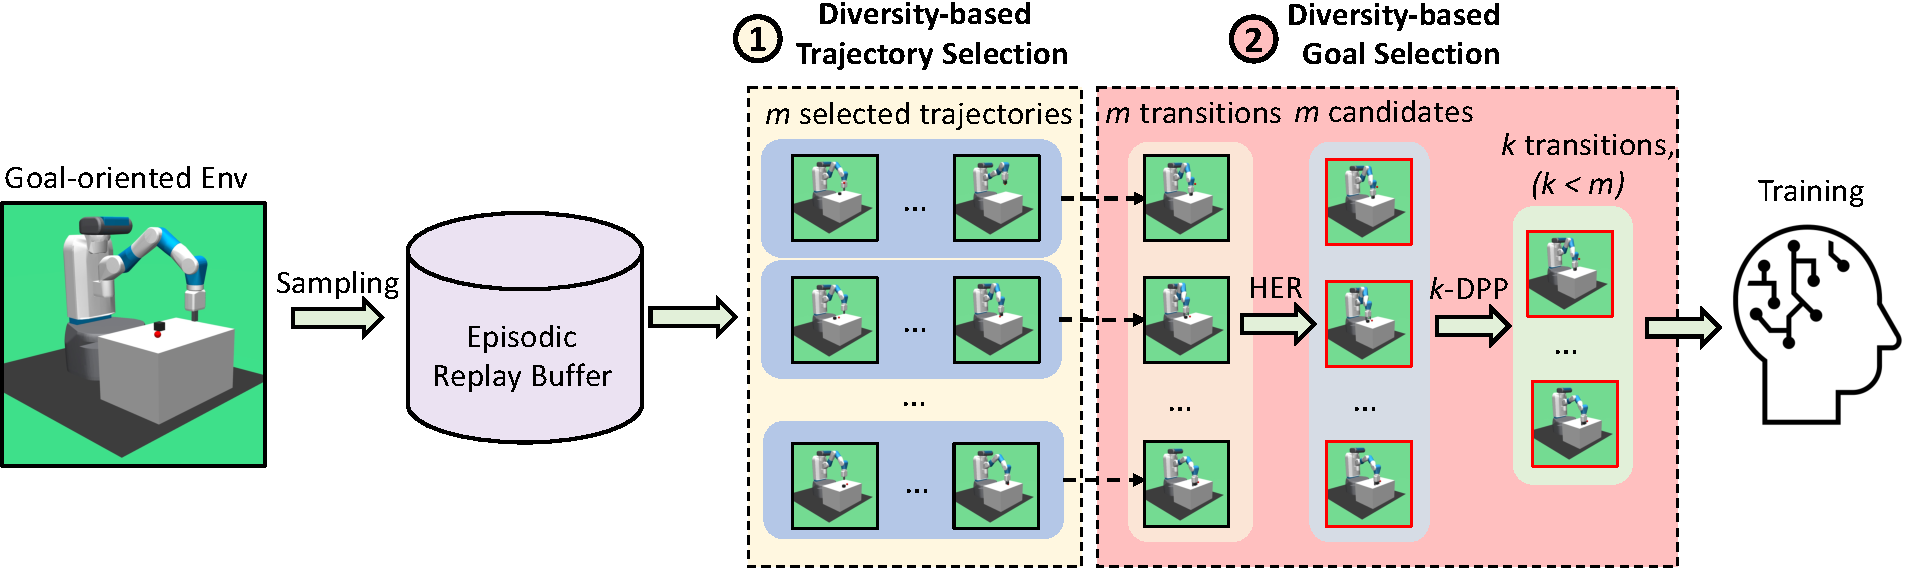
\includegraphics[width=\textwidth]{figures/chapter4/illustration_DTGSH_latest.pdf}
    \caption{Overview of DTGSH. Every time a new episode is completed, its diversity is calculated, and it is stored in the episodic replay buffer. During training, $m$ episodes are sampled according to their diversity-based priority, and then $k$ diverse, hindsight-relabelled transitions are sampled using a $k$-DPP~\cite{kulesza2011k}.}
    \label{fig:illustration_c4}
\end{figure}

\section{Related Work}
The proposed work is built on HER~\cite{andrychowicz2017hindsight} as a way to effectively augment goal-oriented transitions from a replay buffer: to address the problem of sparse rewards, transitions from unsuccessful trajectories are turned into successful ones. HER uses an episodic replay buffer, with uniform sampling over trajectories, and uniform sampling over transitions. However, these samples may be redundant, and many may contribute little to the successful training of the agent.

In the literature, some efforts have been made to increase the efficiency of HER by prioritising more valuable episodes/transitions. Motivated by the work-energy principle in physics, HEBP~\cite{zhao2018energy} assigns higher probability to trajectories in which the target object has higher energy; once the episodes are sampled, the transitions are then sampled uniformly. However, HEBP requires knowing the semantics of the goal space in order to calculate the probability, which is proportional to the sum of the target's potential, kinetic and rotational energies.

CHER~\cite{fang2019curriculum} dynamically controls the sampling of transitions during training based on a mixture of goal proximity and diversity. Firstly, $m$ episodes are uniformly sampled from the episodic replay buffer, and then a minibatch of $k < m$ is sampled according to the current state of the curriculum. The curriculum initially biases sampling to achieved goals that are close to the desired goal (requiring a distance function), and later biases sampling towards diverse goals, using a $k$-nearest neighbour graph and a submodular function to more efficiently sample a diverse subset of goals (using the same distance function).

Other work has expanded HER in orthogonal directions. Hindsight policy gradient \cite{rauber2018hindsight} and episodic self-imitation learning~\cite{dai2020episodic} apply HER to improve the efficiency of goal-oriented on-policy algorithms. Dynamic HER~\cite{fang2018dher} and competitive ER~\cite{liu2018competitive} expand HER to the dynamic goal and multi-agent settings, respectively.

The use of DPPs in RL has been more limited, with applications towards modelling value functions of sets of agents in multiagent RL~\cite{osogami2019determinantal,pmlr-v119-yang20i}, and most closely related to us, finding diverse policies~\cite{parker2020effective}.

\section{Methodology}
We now formally describe the two main components of our method, DTGSH: 1) a diversity-based trajectory selection module to sample valuable trajectories for the further goal selection, and 2) a diversity-based goal selection module to select transitions with diverse goal states from the previously selected trajectories. Together, these select informative transitions from a large area of the goal space, improving the agent's ability to learn and generalise.

\subsection{Diversity-based Trajectory Selection}
We propose a diversity-based prioritisation method to select valuable trajectories for efficient training. Related to HEBP's prioritisation of high-energy trajectories~\cite{zhao2018energy}, we hypothesise that trajectories that achieve diverse goal states $g^{ac}_{t}$ are more valuable for training; however, unlike HEBP, we do not require knowledge of the goal space semantics.

In a robot manipulation task, the agent needs to move a target object from its initial position, $g^{ac}_{1}$, to the target position, $g$. If the agent never moves the object, despite hindsight relabelling it will not be learning information that would directly help in task completion. On the other hand, if the object moves a lot, hindsight relabelling will help the agent learn about meaningful interactions.

In our approach, DPPs are used to model the diversity of achieved goal states $g^{ac}_{t}$ in an episode, or subsets thereof. For a single trajectory $\Tau$ of length $T$, we divide it into several partial trajectories $\tau_{j}$ of length $b$, with achieved goal states $\{g^{ac}_{t}\}_{t=n:n+b-1}$. That is, with a sliding window of $b = 2$, a trajectory $\Tau$ can be divided into $N_p$ partial trajectories:
\begin{equation}
    \Tau_{i} = \{\{\underbrace{g^{ac}_{1}, g^{ac}_{2}}_{\tau_{1}}\}, \{\underbrace{g^{ac}_{2}, g^{ac}_{3}}_{\tau_{2}}\}, \{\underbrace{g^{ac}_{3}, g^{ac}_{4}}_{\tau_{3}}\}, \cdots, \{\underbrace{g^{ac}_{T-1}, g^{ac}_{T}}_{\tau_{N_{p}}}\}\}.
\end{equation}
The diversity $d_{\tau_{j}}$ of each partial trajectory $\tau_{j}$ can be computed as:
\begin{equation}
    d_{\tau_{j}} = \text{det}(\mathbf{L}_{\tau_{j}}), 
\label{eq:partial_div}
\end{equation}
where $\mathbf{L}_{\tau_{j}}$ is the kernel matrix of partial trajectory $\tau_{j}$:
\begin{equation}
    L_{\tau_{j}} = \mathbf{M}^{T}\mathbf{M},
\end{equation}
and $\mathbf{M}=[\hat{g}^{ac}_{n}, \hat{g}^{ac}_{n+1}, \cdots, \hat{g}^{ac}_{n+b-1}]$, where each $\hat{g}^{ac}$ is the $\ell_2$-normalised version of the achieved goal $g^{ac}$~\cite{kulesza2011k}. Finally, the diversity $d_\Tau$ of trajectory $\Tau$ is the sum of the diversity of its $N_p$ constituent partial trajectories:
\begin{equation}
    d_\Tau = \sum_{j=1}^{N_{p}} d_{\tau_{j}}.
\label{eq:total_div}
\end{equation}

Similarly to HEBP~\cite{zhao2018energy}, we use a non-uniform episode sampling strategy. During training, we prioritise sampling episodes proportionally to their diversity; the probability $p(\Tau_{i})$ of sampling trajectory $\Tau_{i}$ from a replay buffer of size $N_{e}$ is:
\begin{equation}
    p(\Tau_{i}) = \frac{d_{\Tau_{i}}}{\sum_{n=1}^{N_{e}} d_{\Tau_{n}}}.
\label{eq:diversity_priority}
\end{equation}

\subsection{Diversity-based Goal Selection}
In prior work~\cite{andrychowicz2017hindsight,zhao2018energy}, after selecting the trajectories from the replay buffer, one transition from each selected trajectory is sampled uniformly to construct a minibatch for training. However, the modified goals $g^{\prime}$ in the minibatch might be similar, resulting in redundant information. In order to form a minibatch with diverse goals for more efficient learning, we use $k$-DPPs~\cite{kulesza2011k} for sampling goals. Compared to the standard DPP, a $k$-DPP is a conditional DPP where the subset $Y$ has a fixed size $k$, with the probability distribution function:
\begin{equation}
    \mathcal{P}_{L}^{k}(\mathbf{Y}=Y) = \frac{\text{det}(\mathbf{L}_{Y})}{\sum_{|Y^{\prime}|=k} \text{det}(\mathbf{L}_{Y^{\prime}})}.
\end{equation}
$k$-DPPs are more appropriate for goal selection with a minibatch of fixed size $k$. Given $m > k$ trajectories sampled from the replay buffer, we first uniformly sample a transition from each of the $m$ trajectories. Finally, a $k$-DPP is used to sample a diverse set of transitions based on the relabelled goals $g'$ (which, in this context, we denote as ``candidate goals''). Figure~\ref{fig:goal_sampling} gives an example of uniform vs. $k$-DPP sampling, demonstrating the increased coverage of the latter. Figure~\ref{fig:kde} provides corresponding estimated density plots; note that the density of the $k$-DPP samples is actually more uniform over the \textit{support} of the candidate goal distribution.
\begin{figure}[h]
    \begin{subfigure}{\textwidth}
        \centering
        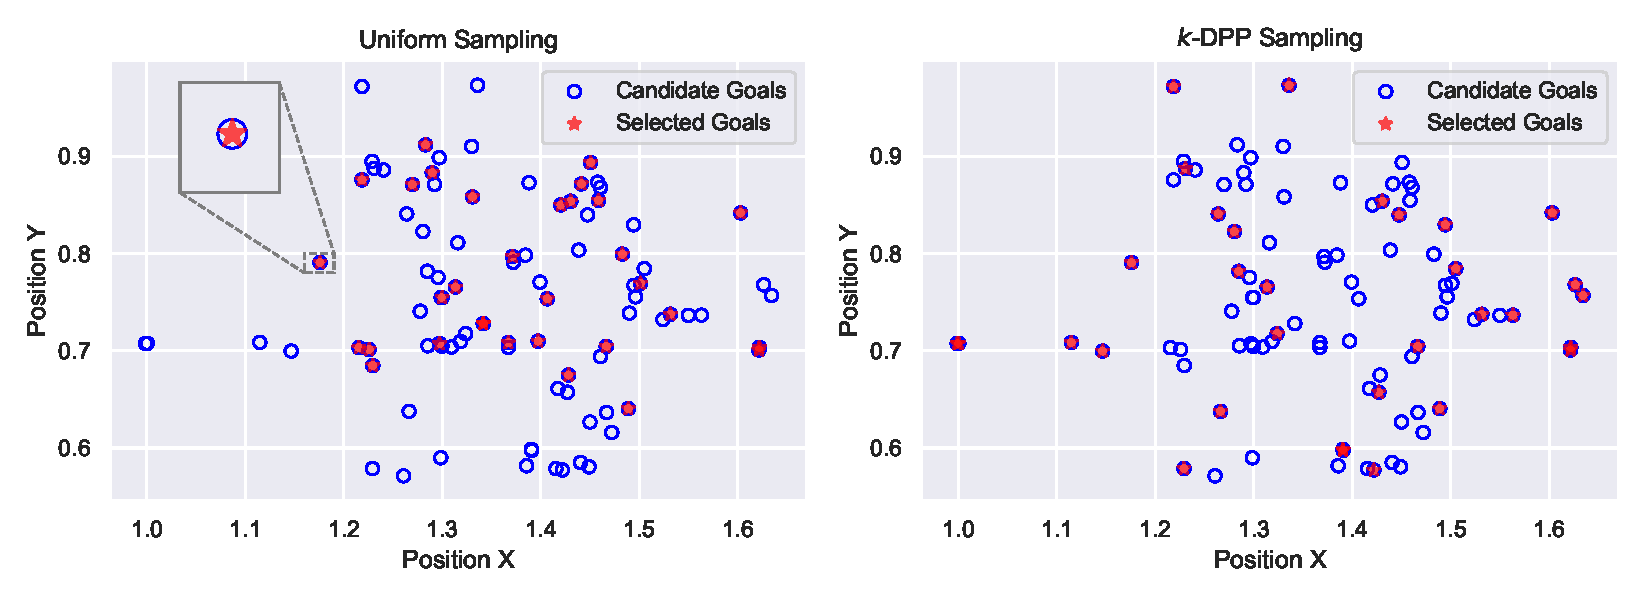
\includegraphics[width=0.9\textwidth]{figures/chapter4/goals_distribution_2d.pdf}
        \caption{Plot of candidate goals and selected goals. $k$-DPP sampling is more likely to sample points from the full span of the goal space.}
        \label{fig:goal_sampling}
    \end{subfigure}
    \begin{subfigure}{\textwidth}
        \centering
        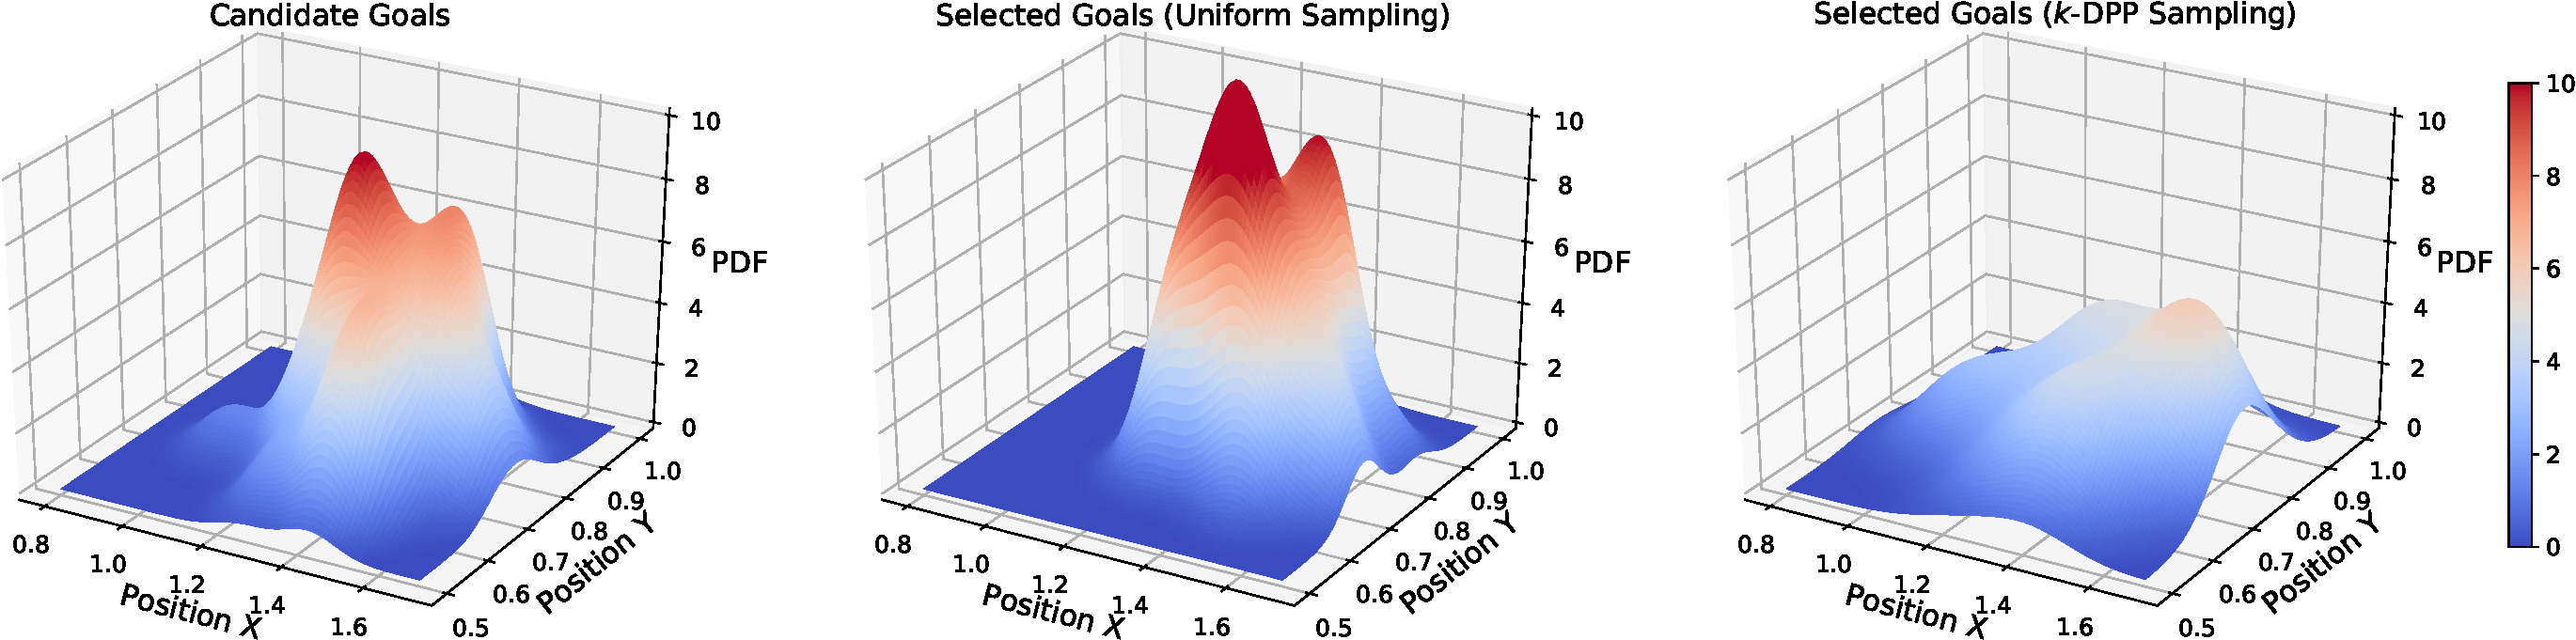
\includegraphics[width=0.9\textwidth]{figures/chapter4/kde.pdf}
        \caption{Kernel density estimation of the distributions of goals. $k$-DPP leads to a more uniform selection of goals over the support of the goal space.}
        \label{fig:kde}
    \end{subfigure}
    \caption{Visualisation of $k=32$ goals selected from $m=100$ candidate goals of the Push task using either uniform sampling or $k$-DPP sampling, respectively. The candidate goals are distributed over a 2D ($xy$) space. Note that  $k$-DPP sampling (right hand plots) results in a broader span of selected goals in $xy$ space compared to uniform sampling (left hand plots).}
\end{figure}

% pseudo code of dpp-sampling
\begin{algorithm}[t!]
\caption{Diversity-based Goal Selection using $k$-DPP}
\label{alg:goal_sample}
\begin{algorithmic}[1]
 \REQUIRE set of $m$ candidate goal states $\mathcal{G}:=\{g_{i}\}_{i=1:m}$, minibatch size $k$
 \STATE $J \leftarrow\varnothing$, $\mathbf{M} \leftarrow  [g_{1}, g_{2}, \cdots, g_{m}]$
 \STATE Calculate the DPP kernel matrix $\mathbf{L}_\mathbf{M}$
 \STATE $\{\boldsymbol{v}_{n}, \lambda_{n}\} \leftarrow \text{EigenDecomposition}(\mathbf{L}_\mathbf{M})$
 %\STATE $e_{k}(\lambda_{1}, \cdots, \lambda_{m}): = \sum\limits_{|J'|=k}\prod_{n\in J'}\lambda_{n}$ \hfill{$\triangleright$ elementary symmetric polynomial: $e^{m}_{k}$}
 \STATE $e_k(\lambda_1,\lambda_2,\dots,\lambda_m) := 
  \sum\limits_{J^{\prime} \subseteq \{1,2,\dots,m\}\atop|J^{\prime}|=k} \prod\limits_{n \in J^{\prime}} \lambda_n$ \hfill{$\triangleright$ elementary symmetric polynomial: $e^{m}_{k}$}
 \FOR{$\mathrm{n} = m, m-1, \cdots, 1$}
 \IF{$u\sim \text{Uniform}[0, 1] < \lambda_{n}\frac{e^{n-1}_{k-1}}{e_{k}^{n}}$}
 \STATE $J \leftarrow J \cup \{n\}$, $k \leftarrow k - 1$
 \IF{$k = 0$}
 \STATE \textbf{break}
 \ENDIF
 \ENDIF
 \ENDFOR
 \STATE $V \leftarrow \{\boldsymbol{v}_{n}\}_{n \in J}$, $B \leftarrow \varnothing$
 \WHILE{$|V| > 0$}
 \STATE Select $g_{i}$ from $\mathcal{G}$ with $p(g_{i}):=\frac{1}{|V|}\sum_{\boldsymbol{v}\in V}(\boldsymbol{v}^{T}\boldsymbol{b}_{i})^{2}$\hfill{$\triangleright$ $\boldsymbol{b}_{i}$ is the $i^{\text{th}}$ standard basis}
 \STATE $B \leftarrow B \cup \{g_{i}\}$
 \STATE $V \leftarrow V_{\perp}$ \hfill{$\triangleright$ an orthonormal basis for the subspace of $V$ orthogonal to $\boldsymbol{b}_{i}$}
 \ENDWHILE
 \RETURN minibatch $B$ with size $k$
\end{algorithmic}
\end{algorithm}

\begin{algorithm}[t!]
\caption{Diversity-based Trajectory and Goal Selection with HER}
\label{alg:main_alg}
\begin{algorithmic}[1]
 \REQUIRE RL environment with episodes of length $T$, number of episodes $N$, off-policy RL algorithm $\mathbb{A}$, episodic replay buffer $\mathcal{B}$, number of algorithm updates $U$, candidate transitions size $m$, minibatch size $k$
 \STATE Initialize the parameters $\theta$ of all models in $\mathbb{A}$
 \STATE $\mathcal{B}\leftarrow\varnothing$
 \FOR{$\mathrm{i} = 1, 2, \cdots, N$}
 \STATE Sample a desired goal $g$ and an initial state $s_{0}$\hfill{$\triangleright$ start a new episode}
 \FOR{$\mathrm{t} = 1, 2, \cdots, T$}
 \STATE Sample an action $a_{t}$ using the policy $\pi(s_{t}, g;\theta)$
 \STATE Execute action $a_{t}$ and get the next state $s_{t+1}$ and achieved goal state $g^{ac}_{t+1}$
 \STATE Calculate $r_{t}$ according to Eq.~\eqref{eq:sparse_reward}
 \STATE Store transition $(s_t, a_t, r_t, s_{t+1}, g, g^{ac}_{t+1})$ in $\mathcal{B}$
 \ENDFOR
 \STATE Calculate the diversity score of current episode $d_{\Tau_{i}}$ using Eq.~\eqref{eq:partial_div} and Eq.~\eqref{eq:total_div}
 \STATE Calculate the diversity-based priority $p(\Tau)$ of each episode in $\mathcal{B}$ using Eq.~\eqref{eq:diversity_priority}
 \FOR{$\mathrm{iteration} = 1, 2, \cdots, U$}
 \STATE Sample $m$ trajectories from $\mathcal{B}$ according to priority $p(\Tau)$
 \STATE Uniformly sample one transition from each of the $m$ trajectories
 \STATE Relabel goals in each transition and recompute the reward to get $m$ candidate transitions $\{(s_{t}, a_{t}, r_{t}^{\prime}, s_{t+1}, g^{\prime})_{n}\}_{n=1:m}$
 \STATE Sample minibatch $B$ with size $k$ from the $m$ candidates using Alg.~\ref{alg:goal_sample}
 \STATE Optimise $\theta$ with minibatch $B$
 \ENDFOR
 \ENDFOR 
\end{algorithmic}
\end{algorithm}

Algorithm~\ref{alg:goal_sample} shows the details of the goal selection subroutine, and Algorithm~\ref{alg:main_alg} gives the overall algorithm for our method, DTGSH.

\section{Experiments}
We evaluate our proposed method, and compare it with current state-of-the-art HER-based algorithms~\cite{andrychowicz2017hindsight,fang2019curriculum,zhao2018energy} on challenging robot manipulation tasks~\cite{plappert2018multi}, pictured in Figure~\ref{fig:env_c4}. Furthermore, we perform ablation studies on our diversity-based trajectory and goal selection modules. Our code is based on OpenAI Baselines\footnote[1]{\url{https://github.com/openai/baselines}}, and is available at: \url{https://github.com/TianhongDai/div-hindsight}.

\begin{figure}
  \begin{subfigure}[t]{0.19\textwidth}
    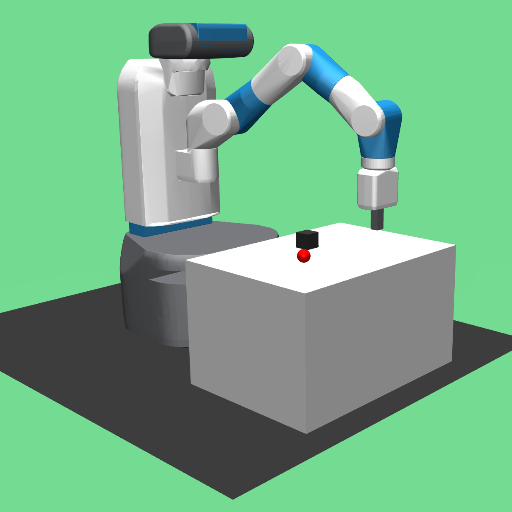
\includegraphics[width=\textwidth]{figures/chapter4/push_resize.png}
    \caption{Push}
    \label{subfig:env_push}
  \end{subfigure}\hfill
  \begin{subfigure}[t]{0.19\textwidth}
    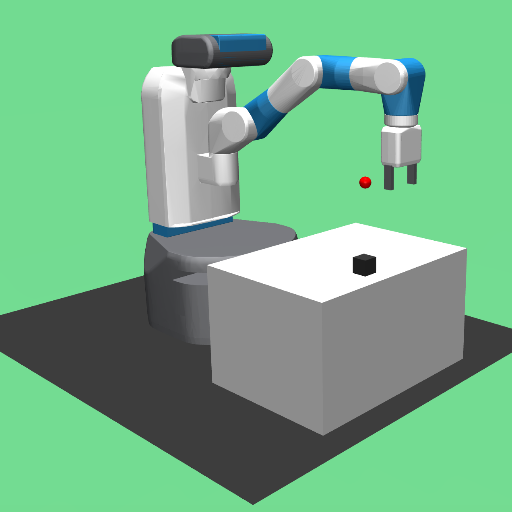
\includegraphics[width=\textwidth]{figures/chapter4/pick_resize.png}
    \caption{Pick$\&$Place}
    \label{subfig:env_pick}
  \end{subfigure}\hfill
  \begin{subfigure}[t]{0.19\textwidth}
    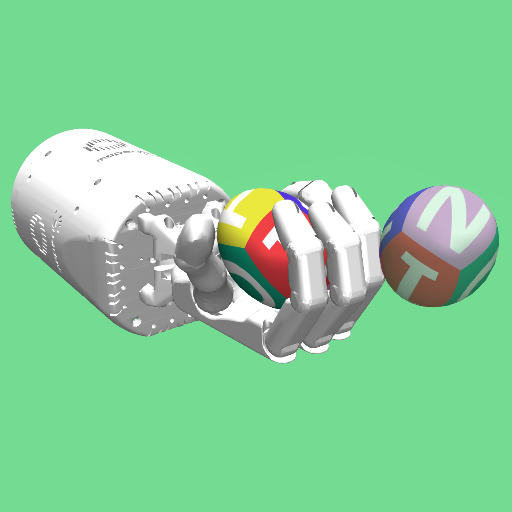
\includegraphics[width=\textwidth]{figures/chapter4/handegg_resize.png}
    \caption{EggFull}
    \label{subfig:env_handegg}
  \end{subfigure}\hfill
  \begin{subfigure}[t]{0.19\textwidth}
    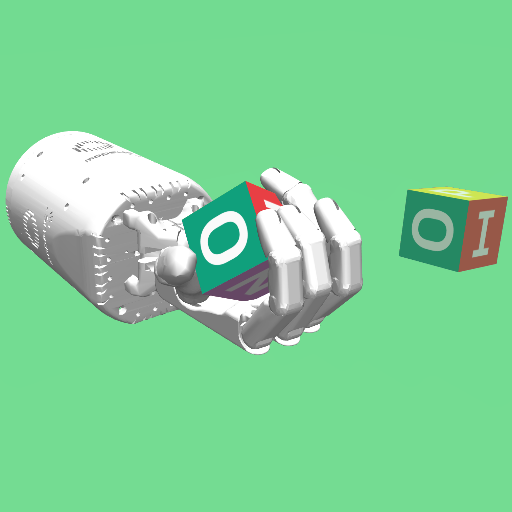
\includegraphics[width=\textwidth]{figures/chapter4/handblock_resize.png}
    \caption{BlockRotate}
    \label{subfig:env_handblock}
  \end{subfigure}\hfill
  \begin{subfigure}[t]{0.19\textwidth}
    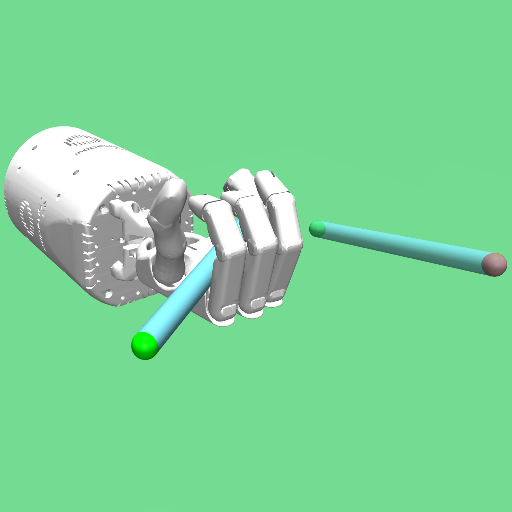
\includegraphics[width=\textwidth]{figures/chapter4/handpen_resize.png}
    \caption{PenRotate}
    \label{subfig:env_handpen}
  \end{subfigure}\hfill
  \caption{Robot manipulation environments. (a-b) use the Fetch robot, and (c-e) use the Shadow Dexterous Hand.} 
  \label{fig:env_c4}
\end{figure}

\subsection{Environments}
The robot manipulation environments used for training and evaluation includes five different tasks. Two tasks use the 7-DoF Fetch robot arm with two-fingers parallel gripper: Push, and Pick\&Place, which both require the agent to move a cube to the target position. The remaining three tasks use a 24-DoF Shadow Dexterous Hand to manipulate an egg, a block and a pen, respectively. The sparse reward function is given by Equation~\eqref{eq:sparse_reward}.

In the Fetch environment, the state $s_{t}$ contains the position and velocity of the joints, and the position and rotation of the cube. Each action, $a_{t}$, is a 4-dimensional vector, with three dimensions specifying the relative position of the gripper, and the final dimension specifying the state of the gripper. The desired goal $g$ is the target position, and the achieved goal $g^{ac}_{t}$ is the position of the cube. Each episode is of length $T = 50$.
%(i.e., open or closed)

In the Shadow Dexterous Hand environment, the state $s_{t}$ contains the position and velocity of the joints. Each action $a_{t}$ is a 20-dimensional vector which specifies the absolute position of 20 non-coupled joints in the hand. The desired goal, $g$, and achieved goal, $g^{ac}_t$, specify the rotation of the object for the block and pen tasks, and the position + rotation of the object for the egg task. Each episode is of length $T = 200$.

\subsection{Experimental Settings}
We base our training setup on CHER~\cite{fang2019curriculum}. We train all agents on minibatches of size $k = 64$ for 50 epochs using MPI for parallelisation over 16 CPU cores; each epoch consists of 1600 ($16 \times 100$) episodes, with evaluation over 160 ($16 \times 10$) episodes at the end of each epoch. Remaining hyperparameters for the baselines are taken from the original respective works~\cite{andrychowicz2017hindsight,fang2019curriculum,zhao2018energy}. Our method, DTGSH, uses partial trajectories of length $b = 2$ and $m = 100$ as the number of candidate goals. 


\subsection{Results on Benchmark Environments}
We compare DTGSH to DDPG~\cite{lillicrapContinuous}, DDPG+HER~\cite{andrychowicz2017hindsight}, DDPG+HEBP~\cite{zhao2018energy} and DDPG+\\CHER~\cite{fang2019curriculum}. Evaluation results are given based on repeated runs with 5 different seeds; we plot the median success rate with upper and lower bounds given by the \nth{75} and \nth{25} percentiles, respectively.

\begin{figure}
\centering
  \begin{subfigure}[t]{0.49\textwidth}
    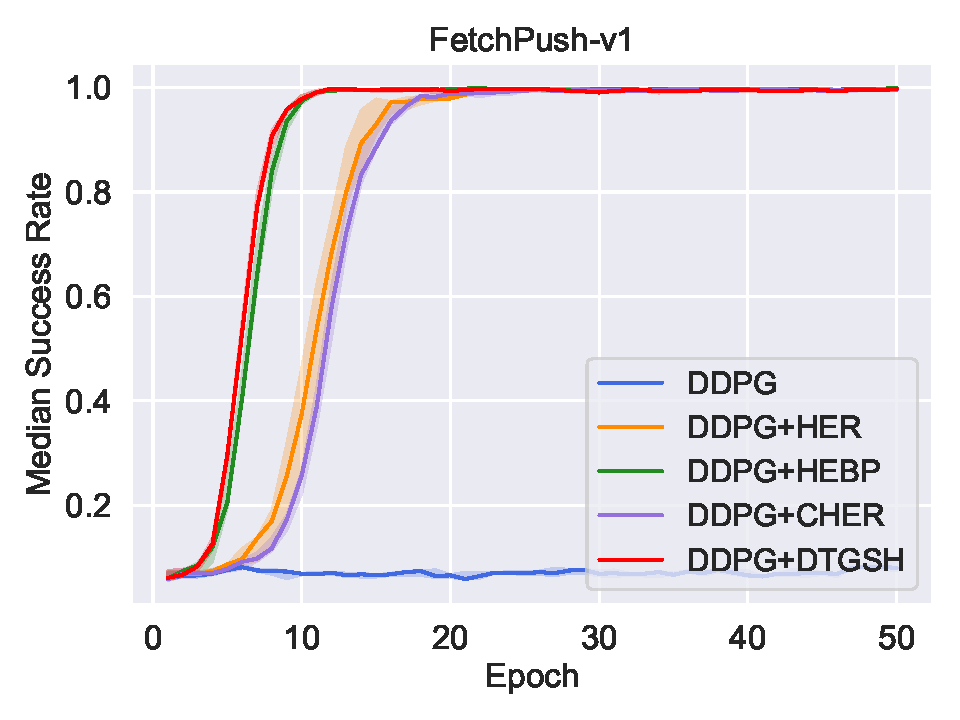
\includegraphics[width=\textwidth]{figures/chapter4/FetchPush-v1.pdf}
    \caption{Push}
    \label{subfig:baseline_push}
  \end{subfigure}\hfill
  \begin{subfigure}[t]{0.49\textwidth}
    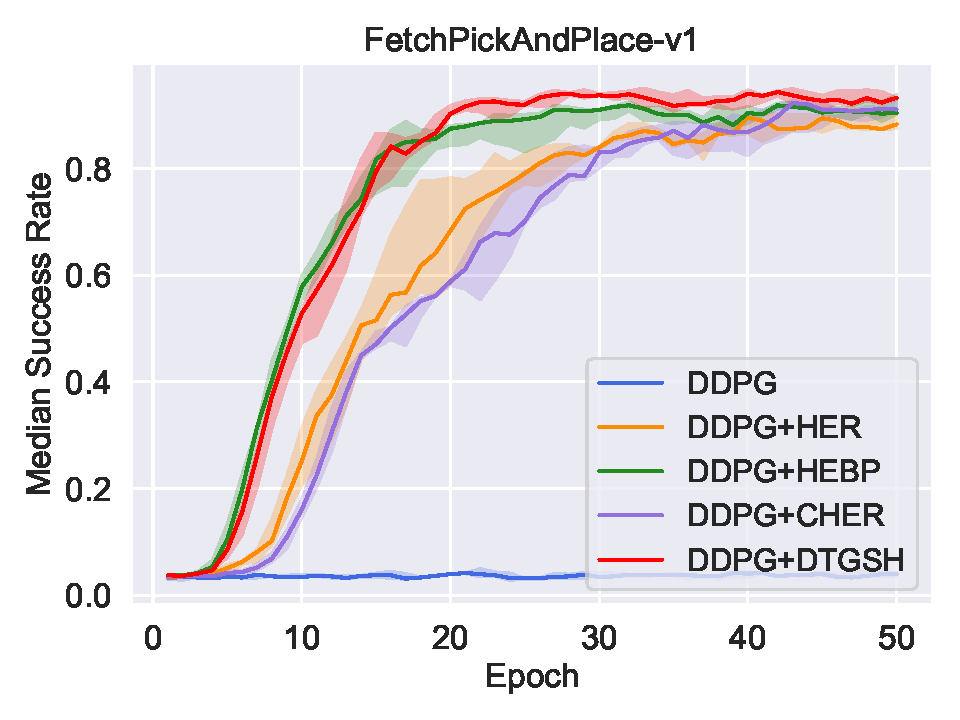
\includegraphics[width=\textwidth]{figures/chapter4/FetchPickAndPlace-v1.pdf}
    \caption{Pick\&Place}
    \label{subfig:baseline_pick}
  \end{subfigure}\hfill
  \begin{subfigure}[t]{0.49\textwidth}
    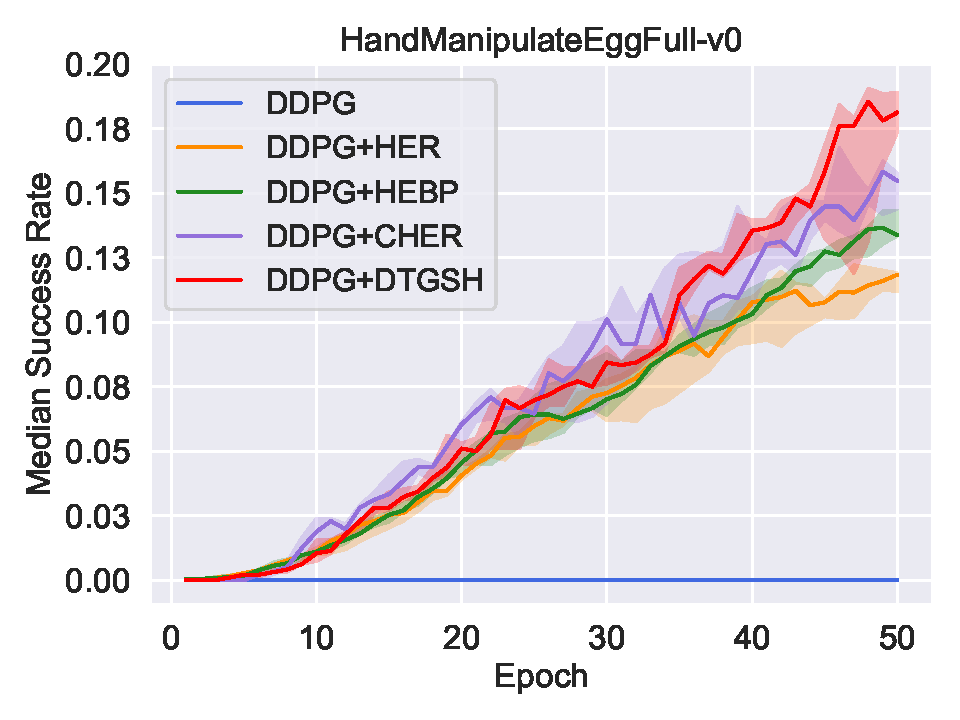
\includegraphics[width=\textwidth]{figures/chapter4/HandManipulateEggFull-v0.pdf}
    \caption{EggFull}
    \label{subfig:baseline_handegg}
  \end{subfigure}\hfill
  \begin{subfigure}[t]{0.49\textwidth}
    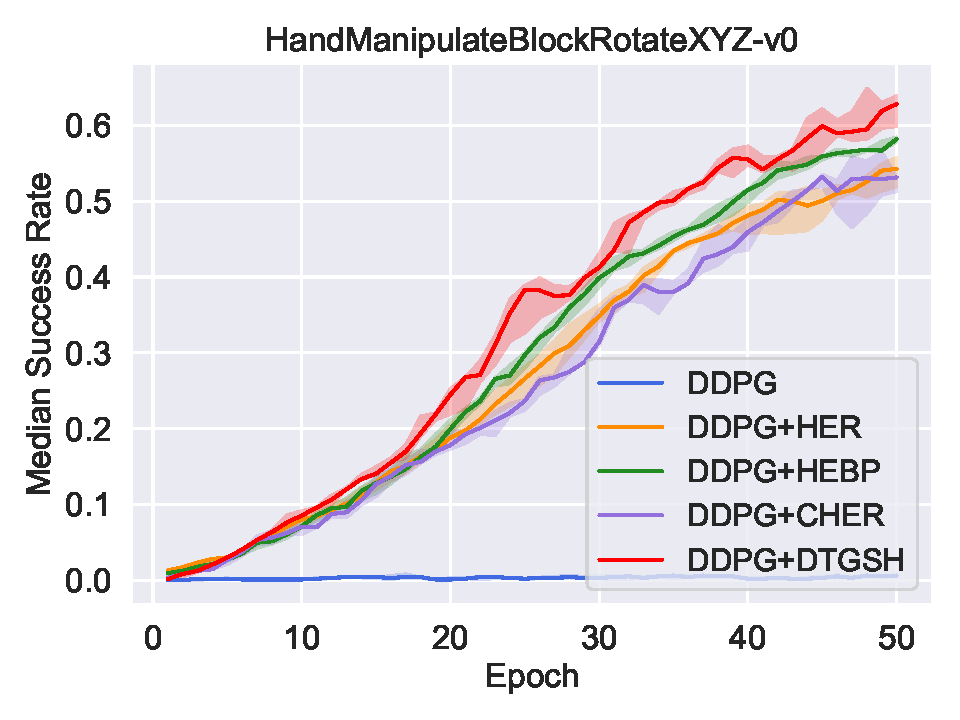
\includegraphics[width=\textwidth]{figures/chapter4/HandManipulateBlockRotateXYZ-v0.pdf}
    \caption{BlockRotate}
    \label{subfig:baseline_handblock}
  \end{subfigure}\hfill
  \begin{subfigure}[t]{0.49\textwidth}
    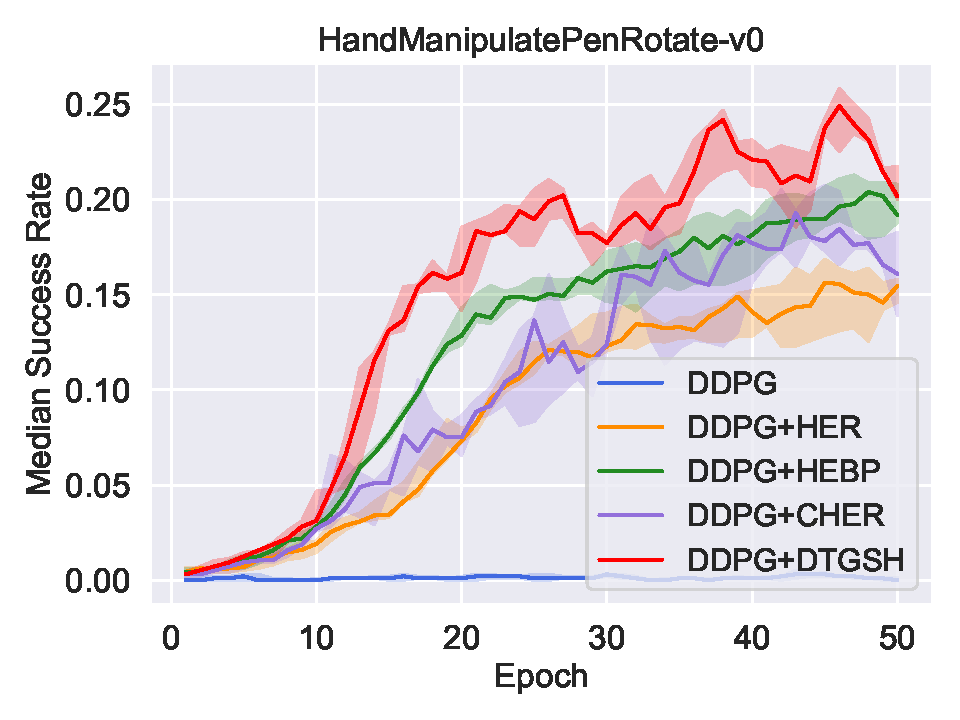
\includegraphics[width=\textwidth]{figures/chapter4/HandManipulatePenRotate-v0.pdf}
    \caption{PenRotate}
    \label{subfig:baseline_handpen}
  \end{subfigure}\hfill
%   \begin{subfigure}[t]{0.49\textwidth}
%     
\includegraphics[width=\textwidth]{figures/chapter4/blank.png}
%   \end{subfigure}\hfill
  \caption{Success rate of DTGSH and baseline approaches. \td{DDPG+DTGSH outpeforms other baselines in all tasks, and without using HER, DDGP cannot even complete the simple Reach task.}} 
  \label{fig:baseline_compare_c4}
\end{figure}

Figure~\ref{fig:baseline_compare_c4} and Table~\ref{tab:benchmark} show the performance of DDPG+DTGSH and baseline approaches on all five tasks. In the Fetch tasks, DDPG+DTGSH and DDPG+HEBP both learn significantly faster than the other methods, while in the Shadow Dexterous Hand tasks DDPG+DTGSH learns the fastest and achieves higher success rates than all other methods. In particular, DDPG cannot solve any tasks without using HER, and CHER performs worse in the Fetch tasks. We believe the results highlight the importance of sampling both diverse trajectories \textit{and} goals, as in our proposed method, DTGSH.
\begin{table}[h]
    \centering
    \resizebox{\textwidth}{!}{
    \begin{tabular}{c|c@{\hskip 0.1in}|c@{\hskip 0.1in}|c|c|c}
    \toprule
         & Push & Pick\&Place & EggFull & BlockRotate & PenRotate \\
        \midrule
        DDPG & 0.09$\pm$0.01 & 0.04$\pm$0.00 & 0.00$\pm$0.00 & 0.01$\pm$0.00 & 0.00$\pm$0.00 \\
        DDPG+HER & \textbf{1.00$\pm$0.00} & 0.89$\pm$0.03 & 0.11$\pm$0.01 & 0.55$\pm$0.04 & 0.15$\pm$0.02 \\
        DDPG+HEBP & \textbf{1.00$\pm$0.00} & 0.91$\pm$0.03 & 0.14$\pm$0.02 & 0.59$\pm$0.02 & 0.20$\pm$0.03\\
        DDPG+CHER & \textbf{1.00$\pm$0.00} & 0.91$\pm$0.04 & 0.15$\pm$0.01 & 0.54$\pm$0.04 & 0.17$\pm$0.03 \\
        \midrule
        DDPG+DTGSH & \textbf{1.00$\pm$0.00} & \textbf{0.94$\pm$0.01} & \textbf{0.17$\pm$0.03} & \textbf{0.62$\pm$0.02} & \textbf{0.21$\pm$0.02}\\
        \bottomrule
    \end{tabular}
    }
    \vspace{0.2em}
    \caption{Final mean success rate $\pm$ standard deviation, with best results in \textbf{bold}.}
    %\vspace{-14mm}
    \label{tab:benchmark}
\end{table}
%\vspace{-15mm}
\subsection{Results on Ablation Studies}
In this section, we perform the following experiments to investigate the effectiveness of each component in DTGSH: 1) diversity-based trajectory selection with HER (DTSH) and diversity-based goal selection with HER (DGSH) are evaluated independently to assess the contribution of each stage, 2) the performance using different partial trajectory lengths $b$, and 3) the performance of using different candidate goal set sizes $m$.
\begin{figure}[h!]
  \centering
  \begin{subfigure}[t]{0.49\textwidth}
    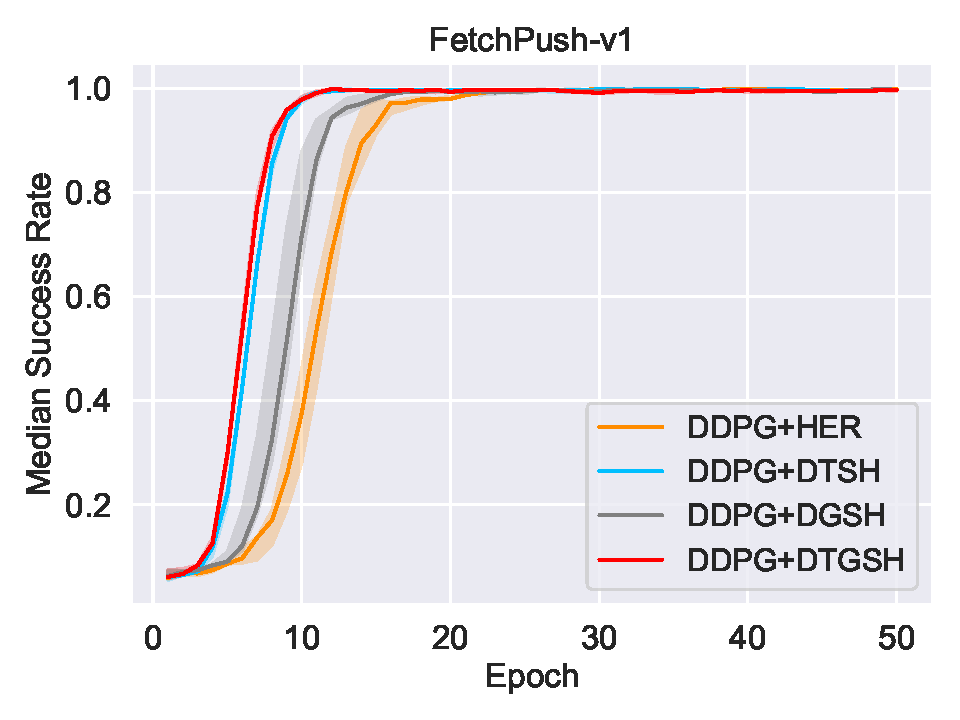
\includegraphics[width=\textwidth]{figures/chapter4/FetchPush-v1_ab1.pdf}
    \caption{Push}
    \label{subfig:baseline_push_ab1}
  \end{subfigure}\hfill
  \begin{subfigure}[t]{0.49\textwidth}
    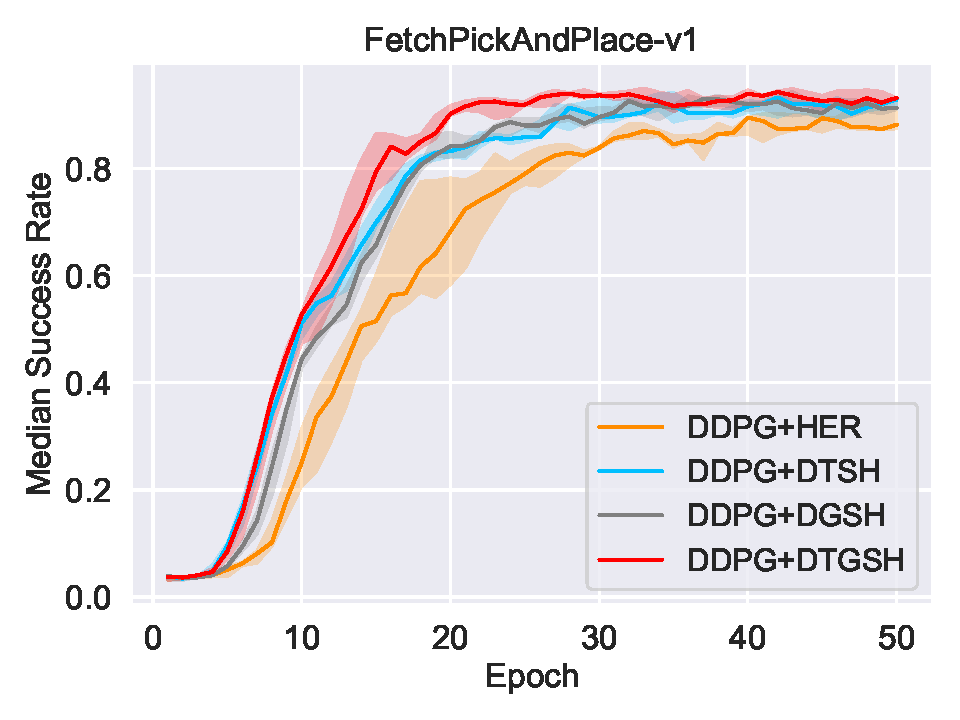
\includegraphics[width=\textwidth]{figures/chapter4/FetchPickAndPlace-v1_ab1.pdf}
    \caption{Pick\&Place}
    \label{subfig:baseline_pick_ab1}
  \end{subfigure}\hfill
  \begin{subfigure}[t]{0.49\textwidth}
    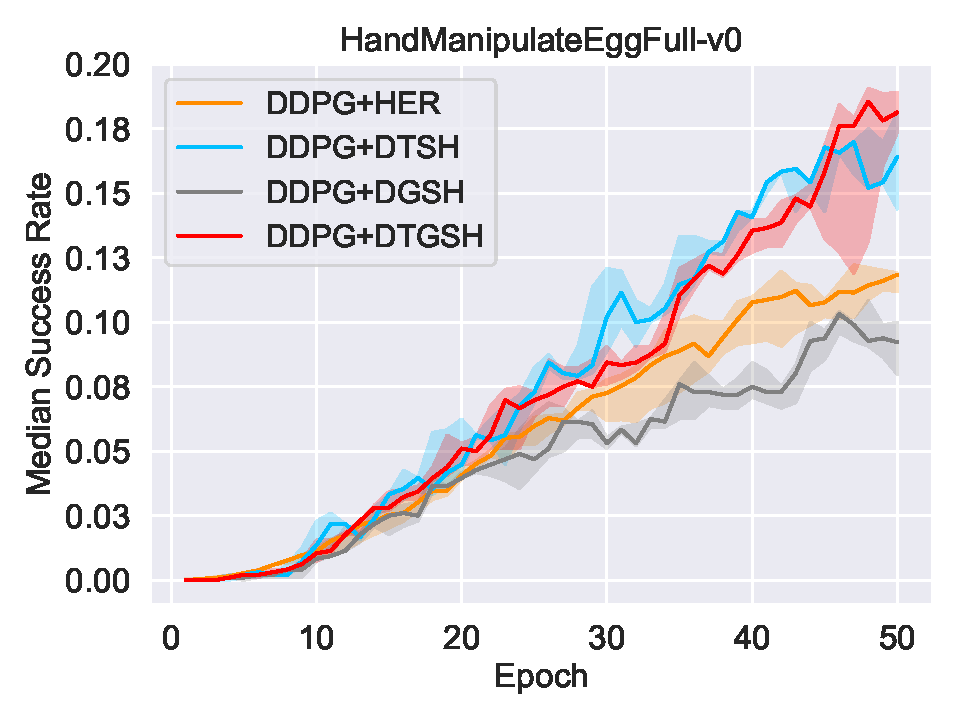
\includegraphics[width=\textwidth]{figures/chapter4/HandManipulateEggFull-v0_ab1.pdf}
    \caption{EggFull}
    \label{subfig:baseline_handegg_ab1}
  \end{subfigure}\hfill
  \begin{subfigure}[t]{0.49\textwidth}
    \includegraphics[width=\textwidth]{figures/chapter4/HandManipulateBlockRotateXYZ-v0_ab1.pdf}
    \caption{BlockRotate}
    \label{subfig:baseline_handblock_ab1}
  \end{subfigure}\hfill
  \begin{subfigure}[t]{0.49\textwidth}
    \includegraphics[width=\textwidth]{figures/chapter4/HandManipulatePenRotate-v0_ab1.pdf}
    \caption{PenRotate}
    \label{subfig:baseline_handpen_ab1}
  \end{subfigure}\hfill
%   \begin{subfigure}[t]{0.33\textwidth}
%     \includegraphics[width=\textwidth]{figures/chapter4/blank.png}
%   \end{subfigure}\hfill
  \caption{Success rate of HER, DTGSH, and ablations DTSH and DGSH. \td{From the results, DTSH outperforms DDPG+HER in all tasks, which verify the efficiency that selecting trajectories with diverse achieved goals for training. DGSH also has better performance than DDPG+HER in three tasks. By combining these two modules together, DTGSH achieves the best performance.} } 
  \label{fig:ablation1}
\end{figure}

Figure~\ref{fig:ablation1} shows the performance of using DTSH and DGSH independently. DDPG+\\DTSH outperforms DDPG+HER substantially in all tasks, which supports the view that sampling trajectories with diverse achieved goals can substantially improve performance. Furthermore, unlike DDPG+HEBP, DTSH does not require knowing the structure of the goal space in order to calculate the energy of the target object; DDPG+DGSH achieves better performance than DDPG+HER in three tasks, and is only worse in one task. DGSH performs better in the environment where it is easier to solve the task (e.g., Fetch tasks), and hence the trajectories selected are more likely to contain useful transitions. However, DTGSH, which is the combination of both modules, performs the best overall.

\begin{figure}[h!]
\centering
  \begin{subfigure}[t]{0.49\textwidth}
    \includegraphics[width=\textwidth]{figures/chapter4/FetchPush-v1_ab2.pdf}
    \caption{Push}
    \label{subfig:baseline_push_ab2}
  \end{subfigure}\hfill
  \begin{subfigure}[t]{0.49\textwidth}
    \includegraphics[width=\textwidth]{figures/chapter4/FetchPickAndPlace-v1_ab2.pdf}
    \caption{Pick\&Place}
    \label{subfig:baseline_pick_ab2}
  \end{subfigure}\hfill
  \begin{subfigure}[t]{0.49\textwidth}
    \includegraphics[width=\textwidth]{figures/chapter4/HandManipulateEggFull-v0_ab2.pdf}
    \caption{EggFull}
    \label{subfig:baseline_handegg_ab2}
  \end{subfigure}\hfill
  \begin{subfigure}[t]{0.49\textwidth}
    \includegraphics[width=\textwidth]{figures/chapter4/HandManipulateBlockRotateXYZ-v0_ab2.pdf}
    \caption{BlockRotate}
    \label{subfig:baseline_handblock_ab2}
  \end{subfigure}\hfill
  \begin{subfigure}[t]{0.49\textwidth}
    \includegraphics[width=\textwidth]{figures/chapter4/HandManipulatePenRotate-v0_ab2.pdf}
    \caption{PenRotate}
    \label{subfig:baseline_handpen_ab2}
  \end{subfigure}\hfill
%   \begin{subfigure}[t]{0.33\textwidth}
%     \includegraphics[width=\textwidth]{figures/chapter4/blank.png}
%   \end{subfigure}\hfill
  \caption{Success rate of DTGSH with different partial trajectory lengths $b$ and different candidate goal set sizes $m$. \td{From the results, when $b \gg 2$, the performance degrades in all tasks. When $m \gg 100$, the performance degrades in the Shadow Dexterous Hand environment.}} 
  \label{fig:ablation2}
\end{figure}

Figure~\ref{fig:ablation2} shows the performance of DDPG+DTGSH with different partial trajectory lengths $b$ and different candidate goal set sizes $m$. In this work, we use $b = 2$ and $m = 100$ as the defaults. Performance degrades with $b \gg 2$, indicating that pairwise diversity is the best for learning in our method. $m \gg 100$ does not affect performance in the Fetch environment, but degrades performance in the Shadow Dexterous Hand environment.

\subsection{Time Complexity}
Table~\ref{tab:time} gives example training times of all of the HER-based algorithms. DTGSH requires an additional calculation of the diversity score of $\mathcal{O}(N_{p}b^3)$ at the end of every training episode, and sampling of $\mathcal{O}(mk^2)$ for each minibatch.
\begin{table}[h!]
    \centering
    \resizebox{0.85\textwidth}{!}{
    \begin{tabular}{c|c|c|c|c}
    \toprule
           & DDPG+HER & DDPG+HEBP & DDPG+CHER & DDPG+DTGSH\\
        \midrule
        Time  & 00:55:08 & 00:56:32 & 03:02:18 & 01:52:30 \\
        \bottomrule
    \end{tabular}
    }
    \vspace{0.2em}
    \caption{Training time (hours:minutes:seconds) of DTGSH and baseline approaches on the Push task for 50 epochs.}
    \label{tab:time}
\end{table}

\section{Discussion}
In this chapter, we introduced diversity-based trajectory and goal selection with hindsight experience replay (DTGSH) to improve the learning efficiency of goal-orientated RL agents in sparse reward settings. Our method can be divided into two stages: 1) valuable trajectories are selected according to diversity-based priority, as modelled by determinantal point processes (DPPs)~\cite{kulesza2012determinantal}, and 2) $k$-DPPs~\cite{kulesza2011k} are leveraged to sample transitions with diverse goal states from previously selected trajectories for training. Our experiments empirically show that DTGSH achieves faster learning and higher final performance in five challenging robot manipulation tasks, compared to previous state-of-the-art approaches~\cite{andrychowicz2017hindsight,fang2019curriculum,zhao2018energy}. Furthermore, unlike prior extensions of hindsight experience replay, DTGSH does not require semantic knowledge of the goal space~\cite{zhao2018energy}, and does not require tuning a curriculum~\cite{fang2019curriculum}.

% body of thesis comes here

\chapter{Conclusion}

\label{ch:conclusions}

\section{Summary of Thesis Achievements}
In this thesis, we have proposed several approaches to improve the sample efficiency of deep reinforcement learning (DRL) in tasks with sparse and delayed rewards. Moreover, we provide a comprehensive quantitative and qualitative analysis on the agents trained with and without domain randomisation (DR) to visualise and explain why DR can improve the robustness of the agents against unseen scenarios. 

Firstly, in \textbf{Chapter}~\ref{ch:esil} and \textbf{Chapter}~\ref{ch:dtgsh}, our methods aim to improve the learning efficiency of goal-oriented RL in continuous control tasks with sparse rewards. In \textbf{Chapter}~\ref{ch:esil}, to overcome the difficulty that the agent rarely achieves positive rewards from the environment, hindsight goal relabelling is leveraged to modify failed trajectories into successful ones. Then, these modified trajectories are used to accelerate the training/exploration in the initial stages of training via a self-imitation learning scheme. In addition, a trajectory selection module and an adaptive weight are proposed to remove redundant hindsight experiences and maintain the balance between the exploration and exploiting. In \textbf{Chapter}~\ref{ch:dtgsh}, we argue that when using hindsight goal relabelling, not all agent's experiences contribute equally to the training, and the naive uniform sampling may lead to inefficient learning. In order to achieve valuable experience, we first sample trajectories according to the diversity of the goal states as modelled by determinantal point processes (DPPs). Then, transitions with diverse goal states are selected from the trajectories by using $k$-DPPs. Extensive experiments in these two chapters demonstrate the effectiveness of our methods and show that our methods achieve state-of-the-art results on several simulated robot manipulation tasks.

Secondly, in \textbf{Chapter}~\ref{ch:daim}, diversity is again used via a mechanism of intrinsic motivation, a diversity-augmented intrinsic motivation is proposed to encourage the agent keep exploring novel states in the environment. This intrinsic reward is formulated based on the diversity of adjacent states, measured under the framework of DPPs. Furthermore, a bi-level optimisation is used to guarantee that when increasing the intrinsic reward to encourage the agent to explore novel states, the extrinsic returns are still maximised. Experimental results show that this method outperforms other baselines on the MuJoCo continuous control tasks with standard and delayed reward settings, and it accelerates exploration in the initial stage of training in the arcade learning environments. 

Finally, in \textbf{Chapter}~\ref{ch:drl_interp}, we investigate the agents trained with and without DR to interpret why the agents trained with DR are more robust to unseen scenarios. In this work, we built two simulated robot environments that provide both visual and proprioceptive inputs. The agents are trained to manipulate the robot arm to reach a specific target with different training conditions (different types of inputs and with or without DR). In order to analyse the trained agents, various previously unseen test conditions are used to evaluate the robustness of the trained agents, and both quantitative and qualitative analysis are applied to provide sufficient insights into the behaviour of the trained agents. We further propose an improved occlusion-based saliency map method to provide better attention maps of the agents at each timestep. \td{From results, we show that the DR agents have better generalisation ability to local visual changes, and also exhibit a degree of robustness to global visual changes. The saliency maps of the DR agents focus more on the target object, while non-DR agents show attention to the distractors. In the layer re-initialisation, DR agents also show significant changes in the parameters, which leads to more robust features. The recurrent ablations also reflect the LSTM is only necessary when DR is activated.} In the end, some recommendations for applying interpretability methods to DRL agents are also suggested. 

%\section{Applications}

%Applications.
\section{Future Work and Potential Applications}
The topic of my thesis focuses on improving sample efficiency in DRL and interpretability in DRL. Thus, this section can be split into two branches: 1) discussion of limitations and potential extensions to the proposed methods. 2) potential applications to solve scientific problems.

\subsection{Limitations and Extensions}
In \textbf{Chapter}~\ref{ch:esil}, the proposed episodic self-imitation learning (ESIL) allows on-policy DRL algorithms (e.g., PPO) and hindsight experience replay (HER) to be combined and can be used to solve continuous control tasks with the sparse rewards. However, this still require more samples for training than off-policy DRL algorithms (e.g., DDPG+HER). One possible future study is to improve the sample efficiency with ESIL. Another future work could incorporate self-imitation learning mechanisms with DDPG+HER. Nair \textit{et al.}~\cite{nair2018overcoming} have already done relevant work, where they collect expert demonstrations for imitation learning. In stead of manually collecting demonstrations, \td{a potential improvement is to utilise} past good trajectories for self-imitation learning in the off-policy DRL paradigm.

In \textbf{Chapter}~\ref{ch:dtgsh}, the diversity-based sampling strategy is only applicable to environments that contain manipulable objects, such as picking and placing a cube at a target position. In the future, we can extend this method to more general goal-oriented tasks, such as navigating an agent to arrive at a target location in a maze~\cite{florensa2018automatic}.

In \textbf{Chapter}~\ref{ch:daim}, the proposed diversity-augmented intrinsic motivation (DAIM) achieves limited performance in the arcade learning environment (ALE), and it is also unable to address hard exploration tasks, such as Montezuma's Revenge. Therefore, \td{tackling such challenging hard exploration tasks is a potential direction for improvement.}

In \textbf{Chapter}~\ref{ch:drl_interp}, the current work focuses solely on the analysis of visual domain randomisation. In the future, we will also analysis the trained agents with dynamic DR (e.g., changing the frictional coefficient.). Furthermore, instead of using a simple reach task as the test environment, we will further develop more complicated tasks for analysing, such as a stacking cube task or a pick and place task, which are more in line with real-world applications.

In addition, although there exist plentiful methods to improve sample efficiency in DRL. However, sample efficiency in DRL is still a challenging problem. Therefore, I will further discuss some interesting and novel directions for my future research work.

Firstly, rather than using HER to address goal-oriented RL problems, C-learning~\cite{eysenbach2020c} provides a new paradigm to solve goal-oriented RL by estimating the probability density over future states. In practice, estimating the probability density function is very difficult, and C-learning estimates this density function indirectly via training a binary classifier to predict if the current state--action pair can generate a specific future state (i.e. the goal state) in the current episode, and the state--action pair has a higher probability of generating the goal state will be assigned with a higher return for training. Extensive experiments also show that C-learning outperforms other baselines in various goal-oriented tasks. Therefore, C-learning proposes a new way to solve goal-oriented RL, and it deserves further investigation.

Another way to improve sample efficiency in DRL is to reuse prior knowledge from previously unseen tasks. This kind of method can differ from imitation learning methods~\cite{bojarski2016end,xu2017end,torabi2018behavioral} which require collecting demonstrations from the same task. Some related methods like meta-learning based RL~\cite{duan2016rl,wang2017learning,finn2017model} and meta-imitation learning~\cite{duan2017one,finn2017one,huang2019continuous} try to leverage prior knowledge from unseen tasks to accelerate the learning of new tasks. Another interesting method called prior accelerated reinforcement (PARROT)~\cite{singh2020parrot}, first pretrains a flow-based generative model that maps the latent variables, which are conditioned on the current state, to an action by using expert demonstrations from the previous unseen tasks. Subsequently, this pretrained generative model can be used as a behaviour prior to facilitate the exploration in the new tasks. Thus, how to efficiently reuse prior knowledge/skills is an interesting research topic in the future.

\subsection{Potential Applications}
\begin{figure}[h]
  \begin{subfigure}[t]{0.24\textwidth}
    \includegraphics[width=\textwidth]{figures/conclusion/real_img.jpg}
    \caption{Microscopy Image}
    \label{subfig:real_img}
  \end{subfigure}\hfill
  \begin{subfigure}[t]{0.24\textwidth}
    \includegraphics[width=\textwidth]{figures/conclusion/synthetic_image_resize.png}
    \caption{Synthetic Image A}
    \label{subfig:synthetic}
  \end{subfigure}\hfill
  \begin{subfigure}[t]{0.24\textwidth}
    \includegraphics[width=\textwidth]{figures/conclusion/CapGAN.png}
    \caption{Synthetic Image B}
    \label{subfig:synthetic_b}
  \end{subfigure}\hfill
  \begin{subfigure}[t]{0.24\textwidth}
    \includegraphics[width=\textwidth]{figures/conclusion/3d_resize.png}
    \caption{3D Synthetic Image}
    \label{subfig:3d_synthetic}
  \end{subfigure}\hfill
  \caption{Examples of different types of axon images. (a) is a real microscopy image, (b) is the basic 2D synthetic axon image, (c) is the 2D synthetic axon image generated by CapsPix2Pix~\cite{bass2018image}, and (d) is the 3D synthetic axon image.} 
  \label{fig:axon_env}
\end{figure}
The recent successful achievement of machine learning for science is AlphaFold~\cite{jumper2021highly}, which leverages state-of-the-art deep learning based techniques to predict the 3D structure of a protein based solely on its genetic sequence, and the predicted structures are far more accurate than the outputs of any previous approaches. Predicting protein structures is important to understand the functionality of proteins in any biological system as well as in the diagnosis and treatment of especially genetic diseases (e.g., Alzheimer). Thus, it is meaningful if DRL can be applied to address some real-world/scientific problems. One potential application of DRL is to track the elongated structure in biomedical/microscopy images, such as axons and blood vessels. Automatically tracking elongated structures is a challenging problem in the field of biomedical imaging. \td{In contrast to segmentation, tracking also allows the establishment of correspondences and state estimation to be performed.} Some existing algorithms, such as Kalman filtering, particle filtering, or semi-heuristic connectivity algorithms, require tuning parameters manually for different datasets. To alleviate the need for hand-engineering trackers for different biomedical image datasets, we
first formulate the task of tracing paths along the centrelines of elongated structures as a RL problem, and then explore the use of DRL to train deep convolutional neural networks (CNNs) to learn tracking policies. Up to now, we have developed a simulated environment that can generate synthetic axon images with customised settings, such as the number of axons, the number of branches, and the type of noise (see Figure~\ref{subfig:synthetic}). To reduce the reality gap between the real microscopy image (see Figure~\ref{subfig:real_img}) and the synthetic image, we have proposed CapsPix2Pix~\cite{bass2018image} to generate more realistic synthetic images (see Figure~\ref{subfig:synthetic_b}). We have proposed two DRL trackers~\cite{dai2019deep,balaram2019maximum} which are able to solve 2D axon tracking and achieve comparable results with state-of-the-art axon tracking method -- Vaa3D~\cite{peng2010v3d}. However, the above DRL trackers \td{do not yet} scale to the 3D axon tracking task (see Figure~\ref{subfig:3d_synthetic}), because they lack effective exploration in the environment. In the future, we will apply different techniques (e.g., intrinsic motivation) to overcome the exploration problems in the 3D tracking task.
%Thus, the intrinsic motivation method can be combined with the DRL tracker, which encourages the agent to explore novel states to find a promising policy and solve the problem.

%Preliminary Results and Future Work.


\appendix
% appendices come here


\addcontentsline{toc}{chapter}{Bibliography}
\bibliographystyle{apalike}
\bibliography{bibliography/bibliography}

\end{document}
